% Generated by Sphinx.
\def\sphinxdocclass{report}
\documentclass[letterpaper,10pt,english]{sphinxmanual}
\usepackage[utf8]{inputenc}
\DeclareUnicodeCharacter{00A0}{\nobreakspace}
\usepackage{cmap}
\usepackage[T1]{fontenc}
\usepackage{babel}
\usepackage{times}
\usepackage[Bjarne]{fncychap}
\usepackage{longtable}
\usepackage{sphinx}
\usepackage{multirow}

\addto\captionsenglish{\renewcommand{\figurename}{Fig. }}
\addto\captionsenglish{\renewcommand{\tablename}{Table }}
\floatname{literal-block}{Listing }



\title{climlab-0.2.13 Documentation Documentation}
\date{February 15, 2016}
\release{0.2.13a}
\author{Moritz Kreuzer}
\newcommand{\sphinxlogo}{}
\renewcommand{\releasename}{Release}
\makeindex

\makeatletter
\def\PYG@reset{\let\PYG@it=\relax \let\PYG@bf=\relax%
    \let\PYG@ul=\relax \let\PYG@tc=\relax%
    \let\PYG@bc=\relax \let\PYG@ff=\relax}
\def\PYG@tok#1{\csname PYG@tok@#1\endcsname}
\def\PYG@toks#1+{\ifx\relax#1\empty\else%
    \PYG@tok{#1}\expandafter\PYG@toks\fi}
\def\PYG@do#1{\PYG@bc{\PYG@tc{\PYG@ul{%
    \PYG@it{\PYG@bf{\PYG@ff{#1}}}}}}}
\def\PYG#1#2{\PYG@reset\PYG@toks#1+\relax+\PYG@do{#2}}

\expandafter\def\csname PYG@tok@gd\endcsname{\def\PYG@tc##1{\textcolor[rgb]{0.63,0.00,0.00}{##1}}}
\expandafter\def\csname PYG@tok@gu\endcsname{\let\PYG@bf=\textbf\def\PYG@tc##1{\textcolor[rgb]{0.50,0.00,0.50}{##1}}}
\expandafter\def\csname PYG@tok@gt\endcsname{\def\PYG@tc##1{\textcolor[rgb]{0.00,0.27,0.87}{##1}}}
\expandafter\def\csname PYG@tok@gs\endcsname{\let\PYG@bf=\textbf}
\expandafter\def\csname PYG@tok@gr\endcsname{\def\PYG@tc##1{\textcolor[rgb]{1.00,0.00,0.00}{##1}}}
\expandafter\def\csname PYG@tok@cm\endcsname{\let\PYG@it=\textit\def\PYG@tc##1{\textcolor[rgb]{0.25,0.50,0.56}{##1}}}
\expandafter\def\csname PYG@tok@vg\endcsname{\def\PYG@tc##1{\textcolor[rgb]{0.73,0.38,0.84}{##1}}}
\expandafter\def\csname PYG@tok@m\endcsname{\def\PYG@tc##1{\textcolor[rgb]{0.13,0.50,0.31}{##1}}}
\expandafter\def\csname PYG@tok@mh\endcsname{\def\PYG@tc##1{\textcolor[rgb]{0.13,0.50,0.31}{##1}}}
\expandafter\def\csname PYG@tok@cs\endcsname{\def\PYG@tc##1{\textcolor[rgb]{0.25,0.50,0.56}{##1}}\def\PYG@bc##1{\setlength{\fboxsep}{0pt}\colorbox[rgb]{1.00,0.94,0.94}{\strut ##1}}}
\expandafter\def\csname PYG@tok@ge\endcsname{\let\PYG@it=\textit}
\expandafter\def\csname PYG@tok@vc\endcsname{\def\PYG@tc##1{\textcolor[rgb]{0.73,0.38,0.84}{##1}}}
\expandafter\def\csname PYG@tok@il\endcsname{\def\PYG@tc##1{\textcolor[rgb]{0.13,0.50,0.31}{##1}}}
\expandafter\def\csname PYG@tok@go\endcsname{\def\PYG@tc##1{\textcolor[rgb]{0.20,0.20,0.20}{##1}}}
\expandafter\def\csname PYG@tok@cp\endcsname{\def\PYG@tc##1{\textcolor[rgb]{0.00,0.44,0.13}{##1}}}
\expandafter\def\csname PYG@tok@gi\endcsname{\def\PYG@tc##1{\textcolor[rgb]{0.00,0.63,0.00}{##1}}}
\expandafter\def\csname PYG@tok@gh\endcsname{\let\PYG@bf=\textbf\def\PYG@tc##1{\textcolor[rgb]{0.00,0.00,0.50}{##1}}}
\expandafter\def\csname PYG@tok@ni\endcsname{\let\PYG@bf=\textbf\def\PYG@tc##1{\textcolor[rgb]{0.84,0.33,0.22}{##1}}}
\expandafter\def\csname PYG@tok@nl\endcsname{\let\PYG@bf=\textbf\def\PYG@tc##1{\textcolor[rgb]{0.00,0.13,0.44}{##1}}}
\expandafter\def\csname PYG@tok@nn\endcsname{\let\PYG@bf=\textbf\def\PYG@tc##1{\textcolor[rgb]{0.05,0.52,0.71}{##1}}}
\expandafter\def\csname PYG@tok@no\endcsname{\def\PYG@tc##1{\textcolor[rgb]{0.38,0.68,0.84}{##1}}}
\expandafter\def\csname PYG@tok@na\endcsname{\def\PYG@tc##1{\textcolor[rgb]{0.25,0.44,0.63}{##1}}}
\expandafter\def\csname PYG@tok@nb\endcsname{\def\PYG@tc##1{\textcolor[rgb]{0.00,0.44,0.13}{##1}}}
\expandafter\def\csname PYG@tok@nc\endcsname{\let\PYG@bf=\textbf\def\PYG@tc##1{\textcolor[rgb]{0.05,0.52,0.71}{##1}}}
\expandafter\def\csname PYG@tok@nd\endcsname{\let\PYG@bf=\textbf\def\PYG@tc##1{\textcolor[rgb]{0.33,0.33,0.33}{##1}}}
\expandafter\def\csname PYG@tok@ne\endcsname{\def\PYG@tc##1{\textcolor[rgb]{0.00,0.44,0.13}{##1}}}
\expandafter\def\csname PYG@tok@nf\endcsname{\def\PYG@tc##1{\textcolor[rgb]{0.02,0.16,0.49}{##1}}}
\expandafter\def\csname PYG@tok@si\endcsname{\let\PYG@it=\textit\def\PYG@tc##1{\textcolor[rgb]{0.44,0.63,0.82}{##1}}}
\expandafter\def\csname PYG@tok@s2\endcsname{\def\PYG@tc##1{\textcolor[rgb]{0.25,0.44,0.63}{##1}}}
\expandafter\def\csname PYG@tok@vi\endcsname{\def\PYG@tc##1{\textcolor[rgb]{0.73,0.38,0.84}{##1}}}
\expandafter\def\csname PYG@tok@nt\endcsname{\let\PYG@bf=\textbf\def\PYG@tc##1{\textcolor[rgb]{0.02,0.16,0.45}{##1}}}
\expandafter\def\csname PYG@tok@nv\endcsname{\def\PYG@tc##1{\textcolor[rgb]{0.73,0.38,0.84}{##1}}}
\expandafter\def\csname PYG@tok@s1\endcsname{\def\PYG@tc##1{\textcolor[rgb]{0.25,0.44,0.63}{##1}}}
\expandafter\def\csname PYG@tok@gp\endcsname{\let\PYG@bf=\textbf\def\PYG@tc##1{\textcolor[rgb]{0.78,0.36,0.04}{##1}}}
\expandafter\def\csname PYG@tok@sh\endcsname{\def\PYG@tc##1{\textcolor[rgb]{0.25,0.44,0.63}{##1}}}
\expandafter\def\csname PYG@tok@ow\endcsname{\let\PYG@bf=\textbf\def\PYG@tc##1{\textcolor[rgb]{0.00,0.44,0.13}{##1}}}
\expandafter\def\csname PYG@tok@sx\endcsname{\def\PYG@tc##1{\textcolor[rgb]{0.78,0.36,0.04}{##1}}}
\expandafter\def\csname PYG@tok@bp\endcsname{\def\PYG@tc##1{\textcolor[rgb]{0.00,0.44,0.13}{##1}}}
\expandafter\def\csname PYG@tok@c1\endcsname{\let\PYG@it=\textit\def\PYG@tc##1{\textcolor[rgb]{0.25,0.50,0.56}{##1}}}
\expandafter\def\csname PYG@tok@kc\endcsname{\let\PYG@bf=\textbf\def\PYG@tc##1{\textcolor[rgb]{0.00,0.44,0.13}{##1}}}
\expandafter\def\csname PYG@tok@c\endcsname{\let\PYG@it=\textit\def\PYG@tc##1{\textcolor[rgb]{0.25,0.50,0.56}{##1}}}
\expandafter\def\csname PYG@tok@mf\endcsname{\def\PYG@tc##1{\textcolor[rgb]{0.13,0.50,0.31}{##1}}}
\expandafter\def\csname PYG@tok@err\endcsname{\def\PYG@bc##1{\setlength{\fboxsep}{0pt}\fcolorbox[rgb]{1.00,0.00,0.00}{1,1,1}{\strut ##1}}}
\expandafter\def\csname PYG@tok@mb\endcsname{\def\PYG@tc##1{\textcolor[rgb]{0.13,0.50,0.31}{##1}}}
\expandafter\def\csname PYG@tok@ss\endcsname{\def\PYG@tc##1{\textcolor[rgb]{0.32,0.47,0.09}{##1}}}
\expandafter\def\csname PYG@tok@sr\endcsname{\def\PYG@tc##1{\textcolor[rgb]{0.14,0.33,0.53}{##1}}}
\expandafter\def\csname PYG@tok@mo\endcsname{\def\PYG@tc##1{\textcolor[rgb]{0.13,0.50,0.31}{##1}}}
\expandafter\def\csname PYG@tok@kd\endcsname{\let\PYG@bf=\textbf\def\PYG@tc##1{\textcolor[rgb]{0.00,0.44,0.13}{##1}}}
\expandafter\def\csname PYG@tok@mi\endcsname{\def\PYG@tc##1{\textcolor[rgb]{0.13,0.50,0.31}{##1}}}
\expandafter\def\csname PYG@tok@kn\endcsname{\let\PYG@bf=\textbf\def\PYG@tc##1{\textcolor[rgb]{0.00,0.44,0.13}{##1}}}
\expandafter\def\csname PYG@tok@o\endcsname{\def\PYG@tc##1{\textcolor[rgb]{0.40,0.40,0.40}{##1}}}
\expandafter\def\csname PYG@tok@kr\endcsname{\let\PYG@bf=\textbf\def\PYG@tc##1{\textcolor[rgb]{0.00,0.44,0.13}{##1}}}
\expandafter\def\csname PYG@tok@s\endcsname{\def\PYG@tc##1{\textcolor[rgb]{0.25,0.44,0.63}{##1}}}
\expandafter\def\csname PYG@tok@kp\endcsname{\def\PYG@tc##1{\textcolor[rgb]{0.00,0.44,0.13}{##1}}}
\expandafter\def\csname PYG@tok@w\endcsname{\def\PYG@tc##1{\textcolor[rgb]{0.73,0.73,0.73}{##1}}}
\expandafter\def\csname PYG@tok@kt\endcsname{\def\PYG@tc##1{\textcolor[rgb]{0.56,0.13,0.00}{##1}}}
\expandafter\def\csname PYG@tok@sc\endcsname{\def\PYG@tc##1{\textcolor[rgb]{0.25,0.44,0.63}{##1}}}
\expandafter\def\csname PYG@tok@sb\endcsname{\def\PYG@tc##1{\textcolor[rgb]{0.25,0.44,0.63}{##1}}}
\expandafter\def\csname PYG@tok@k\endcsname{\let\PYG@bf=\textbf\def\PYG@tc##1{\textcolor[rgb]{0.00,0.44,0.13}{##1}}}
\expandafter\def\csname PYG@tok@se\endcsname{\let\PYG@bf=\textbf\def\PYG@tc##1{\textcolor[rgb]{0.25,0.44,0.63}{##1}}}
\expandafter\def\csname PYG@tok@sd\endcsname{\let\PYG@it=\textit\def\PYG@tc##1{\textcolor[rgb]{0.25,0.44,0.63}{##1}}}

\def\PYGZbs{\char`\\}
\def\PYGZus{\char`\_}
\def\PYGZob{\char`\{}
\def\PYGZcb{\char`\}}
\def\PYGZca{\char`\^}
\def\PYGZam{\char`\&}
\def\PYGZlt{\char`\<}
\def\PYGZgt{\char`\>}
\def\PYGZsh{\char`\#}
\def\PYGZpc{\char`\%}
\def\PYGZdl{\char`\$}
\def\PYGZhy{\char`\-}
\def\PYGZsq{\char`\'}
\def\PYGZdq{\char`\"}
\def\PYGZti{\char`\~}
% for compatibility with earlier versions
\def\PYGZat{@}
\def\PYGZlb{[}
\def\PYGZrb{]}
\makeatother

\renewcommand\PYGZsq{\textquotesingle}

\begin{document}

\maketitle
\tableofcontents
\phantomsection\label{index::doc}


Contents:


\chapter{Introduction}
\label{intro:introduction}\label{intro::doc}\label{intro:welcome-to-the-climlab-documentation}
What is climlab?


\chapter{Download}
\label{download:download}\label{download::doc}

\section{Code}
\label{download:code}
github


\section{Dependencies}
\label{download:dependencies}
numpy, scipy, etc.


\section{Installation}
\label{download:installation}\begin{quote}

\$ pip install climlab
\end{quote}


\section{Source Code}
\label{download:source-code}
\#.. autofunction:: climlab.model.ebm.EBM


\chapter{Models}
\label{models:models}\label{models::doc}

\section{Energy Balance Model}
\label{models:energy-balance-model}

\section{Radiative Convective Model}
\label{models:radiative-convective-model}

\section{Stommelbox Model}
\label{models:stommelbox-model}

\chapter{Tutorial}
\label{tutorial::doc}\label{tutorial:tutorial}
Principles of the new \emph{climlab} API design:
\begin{itemize}
\item {} 
\emph{climlab.Process} object has several iterable dictionaries of named,

\end{itemize}
\begin{description}
\item[{gridded variables:}] \leavevmode\begin{itemize}
\item {} \begin{description}
\item[{\emph{process.state}}] \leavevmode\begin{itemize}
\item {} 
state variables, usually time-dependent

\end{itemize}

\end{description}

\item {} \begin{description}
\item[{\emph{process.input}}] \leavevmode\begin{itemize}
\item {} 
boundary conditions and other gridded quantities independent of the

\end{itemize}

\emph{process}
- often set by a parent \emph{process}

\end{description}

\item {} 
\emph{process.param}  (which are basically just scalar \emph{input})

\item {} \begin{description}
\item[{\emph{process.tendencies}}] \leavevmode\begin{itemize}
\item {} 
iterable \emph{dict} of time-tendencies (d/dt) for each state variable

\end{itemize}

\end{description}

\item {} \begin{description}
\item[{\emph{process.diagnostics}}] \leavevmode\begin{itemize}
\item {} 
any quantity derived from current state

\end{itemize}

\end{description}

\end{itemize}

\end{description}
\begin{itemize}
\item {} 
The \emph{process} is fully described by contents of \emph{state}, \emph{input} and \emph{param}

\end{itemize}

dictionaries. \emph{tendencies} and \emph{diagnostics} are always computable from current
state.
- \emph{climlab} will remain (as much as possible) agnostic about the data formats
\begin{quote}
\begin{itemize}
\item {} 
Variables within the dictionaries will behave as \emph{numpy.ndarray} objects

\item {} 
Grid information and other domain details accessible as attributes

\end{itemize}
\begin{description}
\item[{of each variable}] \leavevmode\begin{itemize}
\item {} 
e.g. Tatm.lat

\item {} 
Shortcuts like \emph{process.lat} will work where these are unambiguous

\end{itemize}

\end{description}
\end{quote}
\begin{itemize}
\item {} \begin{description}
\item[{Many variables will be accessible as process attributes \emph{process.name}}] \leavevmode\begin{itemize}
\item {} 
this restricts to unique field names in the above dictionaries

\end{itemize}

\end{description}

\item {} \begin{description}
\item[{There may be other dictionaries that do have name conflicts}] \leavevmode\begin{itemize}
\item {} 
e.g. dictionary of tendencies, with same keys as \emph{process.state}

\item {} 
These will \emph{not} be accessible as \emph{process.name}

\item {} 
but \emph{will} be accessible as \emph{process.dict\_name.name}

\end{itemize}

(as well as regular dict interface)

\end{description}

\item {} 
There will be a dictionary of named subprocesses \emph{process.subprocess}

\item {} 
Each item in subprocess dict will itself be a \emph{climlab.Process} object

\item {} 
For convenience with interactive work, each subprocess should be accessible

\end{itemize}

as \emph{process.subprocess.name} as well as \emph{process.subprocess{[}'name'{]}}
- \emph{process.compute()} is a method that computes tendencies (d/dt)
\begin{itemize}
\item {} 
returns a dictionary of tendencies for all state variables

\item {} 
keys for this dictionary are same as keys of state dictionary

\item {} 
tendency dictionary is the total tendency including all subprocesses

\item {} 
method only computes d/dt, does not apply changes

\item {} \begin{description}
\item[{thus method is relatively independent of numerical scheme}] \leavevmode\begin{itemize}
\item {} 
may need to make exception for implicit scheme?

\end{itemize}

\end{description}

\item {} \begin{description}
\item[{method \emph{will} update variables in \emph{process.diagnostic}}] \leavevmode\begin{itemize}
\item {} 
will also \emph{gather all diagnostics} from \emph{subprocesses}

\end{itemize}

\end{description}

\end{itemize}
\begin{itemize}
\item {} \begin{description}
\item[{\emph{process.step\_forward()} updates the state variables}] \leavevmode\begin{itemize}
\item {} 
calls \emph{process.compute()} to get current tendencies

\item {} 
implements a particular time-stepping scheme

\item {} 
user interface is agnostic about numerical scheme

\end{itemize}

\end{description}

\item {} \begin{description}
\item[{\emph{process.integrate\_years()} etc will automate time-stepping}] \leavevmode\begin{itemize}
\item {} 
also computation of time-average diagnostics.

\end{itemize}

\end{description}

\item {} 
Every \emph{subprocess} should work independently of its parent \emph{process} given

\end{itemize}
\begin{description}
\item[{appropriate \emph{input}.}] \leavevmode\begin{itemize}
\item {} 
investigating an individual \emph{process} (possibly with its own

\end{itemize}
\begin{description}
\item[{\emph{subprocesses}) isolated from its parent needs to be as simple as doing:}] \leavevmode\begin{itemize}
\item {} 
\emph{newproc = climlab.process\_like(procname.subprocess{[}'subprocname'{]})}

\item {} 
\emph{newproc.compute()}

\item {} 
anything in the \emph{input} dictionary of \emph{subprocname} will remain fixed

\end{itemize}

\end{description}

\end{description}

To do:
- use OrderedDict to hold the subprocess dictionary
\begin{itemize}
\item {} 
order of execution can then be controled by position in dictionary

\end{itemize}


\section{Section}
\label{tutorial:section}
text


\chapter{Documentation for the code}
\label{api/climlab::doc}\label{api/climlab:module-climlab}\label{api/climlab:documentation-for-the-code}\index{climlab (module)}

\section{Subpackages}
\label{api/climlab:subpackages}

\subsection{climlab.convection package}
\label{api/climlab.convection:climlab-convection-package}\label{api/climlab.convection::doc}

\subsubsection{Submodules}
\label{api/climlab.convection:submodules}

\subsubsection{climlab.convection.convadj module}
\label{api/climlab.convection:module-climlab.convection.convadj}\label{api/climlab.convection:climlab-convection-convadj-module}\index{climlab.convection.convadj (module)}\index{Akamaev\_adjustment() (in module climlab.convection.convadj)}

\begin{fulllineitems}
\phantomsection\label{api/climlab.convection:climlab.convection.convadj.Akamaev_adjustment}\pysiglinewithargsret{\code{climlab.convection.convadj.}\bfcode{Akamaev\_adjustment}}{\emph{theta}, \emph{q}, \emph{beta}, \emph{n\_k}, \emph{theta\_k}, \emph{s\_k}, \emph{t\_k}}{}
Single column only.

\end{fulllineitems}

\index{ConvectiveAdjustment (class in climlab.convection.convadj)}

\begin{fulllineitems}
\phantomsection\label{api/climlab.convection:climlab.convection.convadj.ConvectiveAdjustment}\pysiglinewithargsret{\strong{class }\code{climlab.convection.convadj.}\bfcode{ConvectiveAdjustment}}{\emph{adj\_lapse\_rate=None}, \emph{**kwargs}}{}
Bases: {\hyperref[api/climlab.process:climlab.process.time_dependent_process.TimeDependentProcess]{\emph{\code{climlab.process.time\_dependent\_process.TimeDependentProcess}}}}

Convective adjustment process
Instantly returns column to neutral lapse rate

Adjustment includes the surface IF `Ts' is included in the state
dictionary. Otherwise only the atmopsheric temperature is adjusted.

\end{fulllineitems}

\index{convective\_adjustment\_direct() (in module climlab.convection.convadj)}

\begin{fulllineitems}
\phantomsection\label{api/climlab.convection:climlab.convection.convadj.convective_adjustment_direct}\pysiglinewithargsret{\code{climlab.convection.convadj.}\bfcode{convective\_adjustment\_direct}}{\emph{p}, \emph{T}, \emph{c}, \emph{lapserate=6.5}}{}
Convective Adjustment to a specified lapse rate.

Input argument lapserate gives the lapse rate expressed in degrees K per km
(positive means temperature increasing downward).

Default lapse rate is 6.5 K / km.

Returns the adjusted Column temperature.
inputs:
p is pressure in hPa
T is temperature in K
c is heat capacity in in J / m**2 / K

\end{fulllineitems}


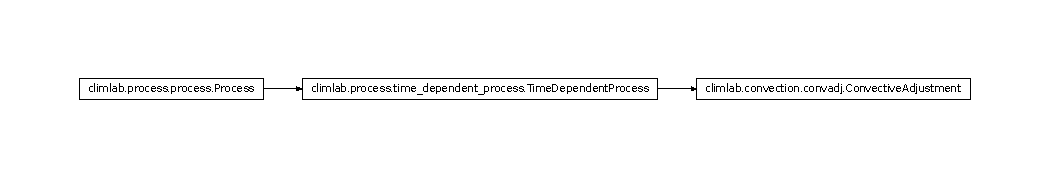
\includegraphics{inheritance-f95e9eb0825078bd01b596c489a95dda67879cbd.pdf}


\subsubsection{Module contents}
\label{api/climlab.convection:module-climlab.convection}\label{api/climlab.convection:module-contents}\index{climlab.convection (module)}

\subsection{climlab.domain package}
\label{api/climlab.domain:climlab-domain-package}\label{api/climlab.domain::doc}

\subsubsection{Submodules}
\label{api/climlab.domain:submodules}

\subsubsection{climlab.domain.axis module}
\label{api/climlab.domain:climlab-domain-axis-module}\label{api/climlab.domain:module-climlab.domain.axis}\index{climlab.domain.axis (module)}\index{Axis (class in climlab.domain.axis)}

\begin{fulllineitems}
\phantomsection\label{api/climlab.domain:climlab.domain.axis.Axis}\pysiglinewithargsret{\strong{class }\code{climlab.domain.axis.}\bfcode{Axis}}{\emph{axis\_type='abstract'}, \emph{num\_points=10}, \emph{points=None}, \emph{bounds=None}}{}
Bases: \href{http://docs.python.org/2.7/library/functions.html\#object}{\code{object}}

Creates a new climlab Axis object.

\textbf{Initialization parameters}

An instance of \code{Axis} is initialized with the following 
arguments \emph{(for detailed information see Object attributes below)}:
\begin{quote}\begin{description}
\item[{Parameters}] \leavevmode\begin{itemize}
\item {} 
\textbf{\texttt{axis\_type}} (\href{http://docs.python.org/2.7/library/functions.html\#str}{\emph{str}}) -- information about the type of axis

\item {} 
\textbf{\texttt{num\_points}} (\href{http://docs.python.org/2.7/library/functions.html\#int}{\emph{int}}) -- number of points on axis

\item {} 
\textbf{\texttt{points}} (\href{http://docs.python.org/2.7/library/array.html\#module-array}{\emph{array}}) -- array with specific points (optional)

\item {} 
\textbf{\texttt{bounds}} (\href{http://docs.python.org/2.7/library/array.html\#module-array}{\emph{array}}) -- array with specific bounds between points (optional)

\end{itemize}

\item[{Raises}] \leavevmode
\code{ValueError}
if \code{axis\_type} is not one of the valid types or 
their euqivalents (see below).

\item[{Raises}] \leavevmode
\code{ValueError}
if \code{points} are given and not array-like.

\item[{Raises}] \leavevmode
\code{ValueError}
if \code{bounds} are given and not array-like.

\end{description}\end{quote}

\textbf{Object attributes}

Following object attributes are generated during initialization:
\begin{quote}\begin{description}
\item[{Variables}] \leavevmode\begin{itemize}
\item {} 
\textbf{\texttt{axis\_type}} (\href{http://docs.python.org/2.7/library/functions.html\#str}{\emph{str}}) -- 
Information about the type of axis. Valid axis types are:
\begin{itemize}
\item {} 
\code{'lev'}

\item {} 
\code{'lat'}

\item {} 
\code{'lon'}

\item {} 
\code{'depth'}

\item {} 
\code{'abstract'} (default)

\end{itemize}


\item {} 
\textbf{\texttt{num\_points}} (\href{http://docs.python.org/2.7/library/functions.html\#int}{\emph{int}}) -- number of points on axis

\item {} 
\textbf{\texttt{units}} (\href{http://docs.python.org/2.7/library/functions.html\#str}{\emph{str}}) -- Unit of the axis. During intialization the unit is 
chosen from the \code{defaultUnits} dictionary (see below).

\item {} 
\textbf{\texttt{points}} (\href{http://docs.python.org/2.7/library/array.html\#module-array}{\emph{array}}) -- array with all points of the axis (grid)

\item {} 
\textbf{\texttt{bounds}} (\href{http://docs.python.org/2.7/library/array.html\#module-array}{\emph{array}}) -- array with all bounds between points (staggered grid)

\item {} 
\textbf{\texttt{delta}} (\href{http://docs.python.org/2.7/library/array.html\#module-array}{\emph{array}}) -- array with spatial differences between bounds

\end{itemize}

\end{description}\end{quote}

\textbf{Axis Types}

Inputs for the \code{axis\_type} like \code{'p'}, \code{'press'}, \code{'pressure'}, 
\code{'P'}, \code{'Pressure'} and \code{'Press'} are refered to as \code{'lev'}.

\code{'Latitude'} and \code{'latitude'} are refered to as \code{'lat'}.

\code{'Longitude'} and \code{'longitude'} are refered to as \code{'lon'}.

And \code{'depth'}, \code{'Depth'}, \code{'waterDepth'}, \code{'water\_depth'} and
\code{'slab'} are refered to as \code{'depth'}.

The \textbf{default units} are:

\begin{Verbatim}[commandchars=\\\{\}]
\PYG{n}{defaultUnits} \PYG{o}{=} \PYG{p}{\PYGZob{}}\PYG{l+s}{\PYGZsq{}}\PYG{l+s}{lev}\PYG{l+s}{\PYGZsq{}}\PYG{p}{:} \PYG{l+s}{\PYGZsq{}}\PYG{l+s}{mb}\PYG{l+s}{\PYGZsq{}}\PYG{p}{,}
                \PYG{l+s}{\PYGZsq{}}\PYG{l+s}{lat}\PYG{l+s}{\PYGZsq{}}\PYG{p}{:} \PYG{l+s}{\PYGZsq{}}\PYG{l+s}{degrees}\PYG{l+s}{\PYGZsq{}}\PYG{p}{,}
                \PYG{l+s}{\PYGZsq{}}\PYG{l+s}{lon}\PYG{l+s}{\PYGZsq{}}\PYG{p}{:} \PYG{l+s}{\PYGZsq{}}\PYG{l+s}{degrees}\PYG{l+s}{\PYGZsq{}}\PYG{p}{,}
                \PYG{l+s}{\PYGZsq{}}\PYG{l+s}{depth}\PYG{l+s}{\PYGZsq{}}\PYG{p}{:} \PYG{l+s}{\PYGZsq{}}\PYG{l+s}{meters}\PYG{l+s}{\PYGZsq{}}\PYG{p}{,}
                \PYG{l+s}{\PYGZsq{}}\PYG{l+s}{abstract}\PYG{l+s}{\PYGZsq{}}\PYG{p}{:} \PYG{l+s}{\PYGZsq{}}\PYG{l+s}{none}\PYG{l+s}{\PYGZsq{}}\PYG{p}{\PYGZcb{}}
\end{Verbatim}

If bounds are not given during initialization, \textbf{default end points} are used:

\begin{Verbatim}[commandchars=\\\{\}]
\PYG{n}{defaultEndPoints} \PYG{o}{=} \PYG{p}{\PYGZob{}}\PYG{l+s}{\PYGZsq{}}\PYG{l+s}{lev}\PYG{l+s}{\PYGZsq{}}\PYG{p}{:} \PYG{p}{(}\PYG{l+m+mf}{0.}\PYG{p}{,} \PYG{n}{climlab}\PYG{o}{.}\PYG{n}{constants}\PYG{o}{.}\PYG{n}{ps}\PYG{p}{)}\PYG{p}{,}
                    \PYG{l+s}{\PYGZsq{}}\PYG{l+s}{lat}\PYG{l+s}{\PYGZsq{}}\PYG{p}{:} \PYG{p}{(}\PYG{o}{\PYGZhy{}}\PYG{l+m+mf}{90.}\PYG{p}{,} \PYG{l+m+mf}{90.}\PYG{p}{)}\PYG{p}{,}
                    \PYG{l+s}{\PYGZsq{}}\PYG{l+s}{lon}\PYG{l+s}{\PYGZsq{}}\PYG{p}{:} \PYG{p}{(}\PYG{l+m+mf}{0.}\PYG{p}{,} \PYG{l+m+mf}{360.}\PYG{p}{)}\PYG{p}{,}
                    \PYG{l+s}{\PYGZsq{}}\PYG{l+s}{depth}\PYG{l+s}{\PYGZsq{}}\PYG{p}{:} \PYG{p}{(}\PYG{l+m+mf}{0.}\PYG{p}{,} \PYG{l+m+mf}{10.}\PYG{p}{)}\PYG{p}{,}
                    \PYG{l+s}{\PYGZsq{}}\PYG{l+s}{abstract}\PYG{l+s}{\PYGZsq{}}\PYG{p}{:} \PYG{p}{(}\PYG{l+m+mi}{0}\PYG{p}{,} \PYG{n}{num\PYGZus{}points}\PYG{p}{)}\PYG{p}{\PYGZcb{}}
\end{Verbatim}

\end{fulllineitems}



\subsubsection{climlab.domain.domain module}
\label{api/climlab.domain:climlab-domain-domain-module}\label{api/climlab.domain:module-climlab.domain.domain}\index{climlab.domain.domain (module)}\index{Atmosphere (class in climlab.domain.domain)}

\begin{fulllineitems}
\phantomsection\label{api/climlab.domain:climlab.domain.domain.Atmosphere}\pysiglinewithargsret{\strong{class }\code{climlab.domain.domain.}\bfcode{Atmosphere}}{\emph{**kwargs}}{}
Bases: {\hyperref[api/climlab.domain:climlab.domain.domain._Domain]{\emph{\code{climlab.domain.domain.\_Domain}}}}

Class for the implementation of a Atmosphere Domain.

\textbf{Object attributes}

Additional to the parent class {\hyperref[api/climlab.domain:climlab.domain.domain._Domain]{\emph{\code{\_Domain}}}}
the following object attribute is modified during initialization:
\begin{quote}\begin{description}
\item[{Variables}] \leavevmode
\textbf{\texttt{domain\_type}} (\href{http://docs.python.org/2.7/library/functions.html\#str}{\emph{str}}) -- is set to \code{'atm'}

\end{description}\end{quote}
\index{set\_heat\_capacity() (climlab.domain.domain.Atmosphere method)}

\begin{fulllineitems}
\phantomsection\label{api/climlab.domain:climlab.domain.domain.Atmosphere.set_heat_capacity}\pysiglinewithargsret{\bfcode{set\_heat\_capacity}}{}{}
Sets the heat capacity of the Atmosphere Domain.

Calls the utils heat capacity function 
{\hyperref[api/climlab.utils:climlab.utils.heat_capacity.atmosphere]{\emph{\code{atmosphere()}}}} and gives the delta 
array of grid points of it's level axis
\code{self.axes{[}'lev'{]}.delta} as input.
\begin{quote}\begin{description}
\item[{Variables}] \leavevmode
{\hyperref[api/climlab.utils:module-climlab.utils.heat_capacity]{\emph{\textbf{\texttt{heat\_capacity}}}}} (\href{http://docs.python.org/2.7/library/array.html\#module-array}{\emph{array}}) -- the ocean domain's heat capacity over 
the \code{'lev'} Axis.

\end{description}\end{quote}

\end{fulllineitems}


\end{fulllineitems}

\index{Ocean (class in climlab.domain.domain)}

\begin{fulllineitems}
\phantomsection\label{api/climlab.domain:climlab.domain.domain.Ocean}\pysiglinewithargsret{\strong{class }\code{climlab.domain.domain.}\bfcode{Ocean}}{\emph{**kwargs}}{}
Bases: {\hyperref[api/climlab.domain:climlab.domain.domain._Domain]{\emph{\code{climlab.domain.domain.\_Domain}}}}

Class for the implementation of an Ocean Domain.

\textbf{Object attributes}

Additional to the parent class {\hyperref[api/climlab.domain:climlab.domain.domain._Domain]{\emph{\code{\_Domain}}}}
the following object attribute is modified during initialization:
\begin{quote}\begin{description}
\item[{Variables}] \leavevmode
\textbf{\texttt{domain\_type}} (\href{http://docs.python.org/2.7/library/functions.html\#str}{\emph{str}}) -- is set to \code{'ocean'}

\end{description}\end{quote}
\index{set\_heat\_capacity() (climlab.domain.domain.Ocean method)}

\begin{fulllineitems}
\phantomsection\label{api/climlab.domain:climlab.domain.domain.Ocean.set_heat_capacity}\pysiglinewithargsret{\bfcode{set\_heat\_capacity}}{}{}
Sets the heat capacity of the Ocean Domain.

Calls the utils heat capacity function 
{\hyperref[api/climlab.utils:climlab.utils.heat_capacity.ocean]{\emph{\code{ocean()}}}} and gives the delta 
array of grid points of it's depth axis
\code{self.axes{[}'depth'{]}.delta} as input.

\textbf{Object attributes}

During method execution following object attribute is modified:
\begin{quote}\begin{description}
\item[{Variables}] \leavevmode
{\hyperref[api/climlab.utils:module-climlab.utils.heat_capacity]{\emph{\textbf{\texttt{heat\_capacity}}}}} (\href{http://docs.python.org/2.7/library/array.html\#module-array}{\emph{array}}) -- the ocean domain's heat capacity over 
the \code{'depth'} Axis.

\end{description}\end{quote}

\end{fulllineitems}


\end{fulllineitems}

\index{SlabAtmosphere (class in climlab.domain.domain)}

\begin{fulllineitems}
\phantomsection\label{api/climlab.domain:climlab.domain.domain.SlabAtmosphere}\pysiglinewithargsret{\strong{class }\code{climlab.domain.domain.}\bfcode{SlabAtmosphere}}{\emph{axes=\textless{}climlab.domain.axis.Axis object\textgreater{}}, \emph{**kwargs}}{}
Bases: {\hyperref[api/climlab.domain:climlab.domain.domain.Atmosphere]{\emph{\code{climlab.domain.domain.Atmosphere}}}}

A class to create a SlabAtmosphere Domain by default.

Initializes the parent {\hyperref[api/climlab.domain:climlab.domain.domain.Atmosphere]{\emph{\code{Atmosphere}}}} class for with a simple axis for a
Slab Atmopshere created by {\hyperref[api/climlab.domain:climlab.domain.domain.make_slabatm_axis]{\emph{\code{make\_slabatm\_axis()}}}} which has just 1 cell 
in height by default.

\end{fulllineitems}

\index{SlabOcean (class in climlab.domain.domain)}

\begin{fulllineitems}
\phantomsection\label{api/climlab.domain:climlab.domain.domain.SlabOcean}\pysiglinewithargsret{\strong{class }\code{climlab.domain.domain.}\bfcode{SlabOcean}}{\emph{axes=\textless{}climlab.domain.axis.Axis object\textgreater{}}, \emph{**kwargs}}{}
Bases: {\hyperref[api/climlab.domain:climlab.domain.domain.Ocean]{\emph{\code{climlab.domain.domain.Ocean}}}}

A class to create a SlabOcean Domain by default.

Initializes the parent {\hyperref[api/climlab.domain:climlab.domain.domain.Ocean]{\emph{\code{Ocean}}}} class for with a simple axis for a
Slab Ocean created by {\hyperref[api/climlab.domain:climlab.domain.domain.make_slabocean_axis]{\emph{\code{make\_slabocean\_axis()}}}} which has just 1 cell 
in depth by default.

\end{fulllineitems}

\index{\_Domain (class in climlab.domain.domain)}

\begin{fulllineitems}
\phantomsection\label{api/climlab.domain:climlab.domain.domain._Domain}\pysiglinewithargsret{\strong{class }\code{climlab.domain.domain.}\bfcode{\_Domain}}{\emph{axes=None}, \emph{**kwargs}}{}
Bases: \href{http://docs.python.org/2.7/library/functions.html\#object}{\code{object}}

Private parent class for domains.

\emph{more details about domains come here}

\textbf{Initialization parameters}

An instance of \code{\_Domain} is initialized with the following 
arguments:
\begin{quote}\begin{description}
\item[{Parameters}] \leavevmode
\textbf{\texttt{axes}} (dict or class:\emph{climlab.domain.axis.Axis}) -- Axis object or dictionary of Axis object where domain will
be defined on.

\end{description}\end{quote}

\textbf{Object attributes}

Following object attributes are generated during initialization:
\begin{quote}\begin{description}
\item[{Variables}] \leavevmode\begin{itemize}
\item {} 
\textbf{\texttt{domain\_type}} (\href{http://docs.python.org/2.7/library/functions.html\#str}{\emph{str}}) -- Set to \code{'undefined'}.

\item {} 
\textbf{\texttt{axes}} (\href{http://docs.python.org/2.7/library/stdtypes.html\#dict}{\emph{dict}}) -- A dictionary of the domains axes. Created by
{\hyperref[api/climlab.domain:climlab.domain.domain._Domain._make_axes_dict]{\emph{\code{\_make\_axes\_dict()}}}} called with input 
argument \code{axes}

\item {} 
\textbf{\texttt{numdims}} (\href{http://docs.python.org/2.7/library/functions.html\#int}{\emph{int}}) -- Number of class:\emph{\textasciitilde{}climlab.domain.Axis} objects
in \code{self.axes} dictionary.

\item {} 
\textbf{\texttt{ax\_index}} (\href{http://docs.python.org/2.7/library/stdtypes.html\#dict}{\emph{dict}}) -- 
A dictionary of domain axes and their corresponding index
in an ordered list of the axes with:
\begin{itemize}
\item {} 
\code{'lev'} or \code{'depth'} is last

\item {} 
\code{'lat'} is second last

\end{itemize}


\item {} 
\textbf{\texttt{shape}} (\href{http://docs.python.org/2.7/library/functions.html\#tuple}{\emph{tuple}}) -- Number of points of all domain axes. Order in 
tuple given by \code{self.ax\_index}.

\item {} 
{\hyperref[api/climlab.utils:module-climlab.utils.heat_capacity]{\emph{\textbf{\texttt{heat\_capacity}}}}} (\href{http://docs.python.org/2.7/library/array.html\#module-array}{\emph{array}}) -- the domain's heat capacity over axis specified 
in function call of {\hyperref[api/climlab.domain:climlab.domain.domain._Domain.set_heat_capacity]{\emph{\code{set\_heat\_capacity()}}}}

\end{itemize}

\end{description}\end{quote}
\index{\_make\_axes\_dict() (climlab.domain.domain.\_Domain method)}

\begin{fulllineitems}
\phantomsection\label{api/climlab.domain:climlab.domain.domain._Domain._make_axes_dict}\pysiglinewithargsret{\bfcode{\_make\_axes\_dict}}{\emph{axes}}{}
Makes an axes dictionary.

\begin{notice}{note}{Note:}
In case the input is \code{None}, the dictionary \code{\{'empty': None\}}
is returned.
\end{notice}

\textbf{Function-call argument}
\begin{quote}\begin{description}
\item[{Parameters}] \leavevmode
\textbf{\texttt{axes}} (dict or single instance of class:\emph{\textasciitilde{}climlab.domain.Axis} object
or \code{None}) -- axes input

\item[{Raises}] \leavevmode
\code{ValueError}  if input is not an instance of Axis class 
or a dictionary of Axis objetcs

\item[{Returns}] \leavevmode
dictionary of input axes

\item[{Return type}] \leavevmode
\href{http://docs.python.org/2.7/library/stdtypes.html\#dict}{dict}

\end{description}\end{quote}

\end{fulllineitems}

\index{set\_heat\_capacity() (climlab.domain.domain.\_Domain method)}

\begin{fulllineitems}
\phantomsection\label{api/climlab.domain:climlab.domain.domain._Domain.set_heat_capacity}\pysiglinewithargsret{\bfcode{set\_heat\_capacity}}{}{}
A dummy function to set the heat capacity of a domain.

\emph{Should be overridden by daugter classes.}

\end{fulllineitems}


\end{fulllineitems}

\index{box\_model\_domain() (in module climlab.domain.domain)}

\begin{fulllineitems}
\phantomsection\label{api/climlab.domain:climlab.domain.domain.box_model_domain}\pysiglinewithargsret{\code{climlab.domain.domain.}\bfcode{box\_model\_domain}}{\emph{num\_points=2}, \emph{**kwargs}}{}
Creates a box model domain (a single abstract axis).
\begin{quote}\begin{description}
\item[{Parameters}] \leavevmode
\textbf{\texttt{num\_points}} (\href{http://docs.python.org/2.7/library/functions.html\#int}{\emph{int}}) -- number of boxes {[}default: 2{]}

\item[{Returns}] \leavevmode
Domain with single axis of type \code{'abstract'} 
and \code{self.domain\_type = 'box'}

\item[{Return type}] \leavevmode
{\hyperref[api/climlab.domain:climlab.domain.domain._Domain]{\emph{\code{\_Domain}}}}

\end{description}\end{quote}

\end{fulllineitems}

\index{make\_slabatm\_axis() (in module climlab.domain.domain)}

\begin{fulllineitems}
\phantomsection\label{api/climlab.domain:climlab.domain.domain.make_slabatm_axis}\pysiglinewithargsret{\code{climlab.domain.domain.}\bfcode{make\_slabatm\_axis}}{\emph{num\_points=1}}{}
Convenience method to create a simple axis for a slab atmosphere.

\textbf{Function-call argument}
\begin{quote}\begin{description}
\item[{Parameters}] \leavevmode
\textbf{\texttt{num\_points}} (\href{http://docs.python.org/2.7/library/functions.html\#int}{\emph{int}}) -- number of points for the slabatmosphere Axis {[}default: 1{]}

\item[{Returns}] \leavevmode
an Axis with \code{axis\_type='lev'} and \code{num\_points=num\_points}

\item[{Return type}] \leavevmode
class:\emph{climlab.domain.axis.Axis}

\end{description}\end{quote}

\end{fulllineitems}

\index{make\_slabocean\_axis() (in module climlab.domain.domain)}

\begin{fulllineitems}
\phantomsection\label{api/climlab.domain:climlab.domain.domain.make_slabocean_axis}\pysiglinewithargsret{\code{climlab.domain.domain.}\bfcode{make\_slabocean\_axis}}{\emph{num\_points=1}}{}
Convenience method to create a simple axis for a slab ocean.

\textbf{Function-call argument}
\begin{quote}\begin{description}
\item[{Parameters}] \leavevmode
\textbf{\texttt{num\_points}} (\href{http://docs.python.org/2.7/library/functions.html\#int}{\emph{int}}) -- number of points for the slabocean Axis {[}default: 1{]}

\item[{Returns}] \leavevmode
an Axis with \code{axis\_type='depth'} and \code{num\_points=num\_points}

\item[{Return type}] \leavevmode
class:\emph{climlab.domain.axis.Axis}

\end{description}\end{quote}

\end{fulllineitems}

\index{single\_column() (in module climlab.domain.domain)}

\begin{fulllineitems}
\phantomsection\label{api/climlab.domain:climlab.domain.domain.single_column}\pysiglinewithargsret{\code{climlab.domain.domain.}\bfcode{single\_column}}{\emph{num\_lev=30}, \emph{water\_depth=1.0}, \emph{lev=None}, \emph{**kwargs}}{}
Creates domains for a single column of atmosphere overlying a slab of water.

Can also pass a pressure array or pressure level axis object specified in \code{lev}.

If argument \code{lev} is not \code{None} then function tries to build a level axis
and \code{num\_lev} is ignored.

\textbf{Function-call argument}
\begin{quote}\begin{description}
\item[{Parameters}] \leavevmode\begin{itemize}
\item {} 
\textbf{\texttt{num\_lev}} (\href{http://docs.python.org/2.7/library/functions.html\#int}{\emph{int}}) -- number of pressure levels
(evenly spaced from surface to TOA) {[}default: 30{]}

\item {} 
\textbf{\texttt{water\_depth}} (\href{http://docs.python.org/2.7/library/functions.html\#float}{\emph{float}}) -- depth of the ocean slab {[}default: 1.{]}

\item {} 
\textbf{\texttt{lev}} (class:\emph{climlab.domain.axis.Axis} or pressure array) -- specification for height axis (optional)

\end{itemize}

\item[{Raises}] \leavevmode
\code{ValueError}  if \emph{lev} is given but neither Axis 
nor pressure array.

\item[{Returns}] \leavevmode
a list of 2 Domain objects (slab ocean, atmosphere)

\item[{Return type}] \leavevmode
\href{http://docs.python.org/2.7/library/functions.html\#list}{\code{list}} of {\hyperref[api/climlab.domain:climlab.domain.domain.SlabOcean]{\emph{\code{SlabOcean}}}}, {\hyperref[api/climlab.domain:climlab.domain.domain.SlabAtmosphere]{\emph{\code{SlabAtmosphere}}}}

\item[{Example}] \leavevmode
\begin{Verbatim}[commandchars=\\\{\}]
\PYG{k+kn}{from} \PYG{n+nn}{climlab} \PYG{k+kn}{import} \PYG{n}{domain}

\PYG{n}{sfc}\PYG{p}{,} \PYG{n}{atm} \PYG{o}{=} \PYG{n}{domain}\PYG{o}{.}\PYG{n}{single\PYGZus{}column}\PYG{p}{(}\PYG{p}{)}
\PYG{c}{\PYGZsh{} or}
\PYG{n}{sfc}\PYG{p}{,} \PYG{n}{atm} \PYG{o}{=} \PYG{n}{domain}\PYG{o}{.}\PYG{n}{single\PYGZus{}column}\PYG{p}{(}\PYG{n}{num\PYGZus{}lev}\PYG{o}{=}\PYG{l+m+mi}{2}\PYG{p}{,} \PYG{n}{water\PYGZus{}depth}\PYG{o}{=}\PYG{l+m+mf}{10.}\PYG{p}{)}
\PYG{k}{print} \PYG{n}{sfc}\PYG{p}{,} \PYG{n}{atm}
\end{Verbatim}

\end{description}\end{quote}

\end{fulllineitems}

\index{zonal\_mean\_column() (in module climlab.domain.domain)}

\begin{fulllineitems}
\phantomsection\label{api/climlab.domain:climlab.domain.domain.zonal_mean_column}\pysiglinewithargsret{\code{climlab.domain.domain.}\bfcode{zonal\_mean\_column}}{\emph{num\_lat=90}, \emph{num\_lev=30}, \emph{water\_depth=10.0}, \emph{lat=None}, \emph{lev=None}, \emph{**kwargs}}{}
Creates two Domains with one water cell, a latitude axis and 
a level/height axis.
\begin{itemize}
\item {} 
SlabOcean:    one water cell and a latitude axis above 
(similar to {\hyperref[api/climlab.domain:climlab.domain.domain.zonal_mean_surface]{\emph{\code{zonal\_mean\_surface()}}}})

\item {} 
Atmosphere: a latitude axis and a level/height axis (two dimensional)

\end{itemize}

\textbf{Function-call argument}
\begin{quote}\begin{description}
\item[{Parameters}] \leavevmode\begin{itemize}
\item {} 
\textbf{\texttt{num\_lat}} (\href{http://docs.python.org/2.7/library/functions.html\#int}{\emph{int}}) -- number of latitude points on the axis
{[}default: 90{]}

\item {} 
\textbf{\texttt{num\_lev}} (\href{http://docs.python.org/2.7/library/functions.html\#int}{\emph{int}}) -- number of pressure levels
(evenly spaced from surface to TOA) {[}default: 30{]}

\item {} 
\textbf{\texttt{water\_depth}} (\href{http://docs.python.org/2.7/library/functions.html\#float}{\emph{float}}) -- depth of the water cell (slab ocean) {[}default: 10.{]}

\item {} 
\textbf{\texttt{lat}} (class:\emph{climlab.domain.axis.Axis} or latitude array) -- specification for latitude axis (optional)

\item {} 
\textbf{\texttt{lev}} (class:\emph{climlab.domain.axis.Axis} or pressure array) -- specification for height axis (optional)

\end{itemize}

\item[{Raises}] \leavevmode
\code{ValueError}  if \emph{lat} is given but neither Axis nor latitude array.

\item[{Raises}] \leavevmode
\code{ValueError}  if \emph{lev} is given but neither Axis nor pressure array.

\item[{Returns}] \leavevmode
a list of 2 Domain objects (slab ocean, atmosphere)

\item[{Return type}] \leavevmode
\href{http://docs.python.org/2.7/library/functions.html\#list}{\code{list}} of {\hyperref[api/climlab.domain:climlab.domain.domain.SlabOcean]{\emph{\code{SlabOcean}}}}, {\hyperref[api/climlab.domain:climlab.domain.domain.Atmosphere]{\emph{\code{Atmosphere}}}}

\end{description}\end{quote}

\end{fulllineitems}

\index{zonal\_mean\_surface() (in module climlab.domain.domain)}

\begin{fulllineitems}
\phantomsection\label{api/climlab.domain:climlab.domain.domain.zonal_mean_surface}\pysiglinewithargsret{\code{climlab.domain.domain.}\bfcode{zonal\_mean\_surface}}{\emph{num\_lat=90}, \emph{water\_depth=10.0}, \emph{lat=None}, \emph{**kwargs}}{}
Creates a Domain with one water cell and a latitude axis above.

Domain has a single heat capacity according to the specified water depth.

\textbf{Function-call argument}
\begin{quote}\begin{description}
\item[{Parameters}] \leavevmode\begin{itemize}
\item {} 
\textbf{\texttt{num\_lat}} (\href{http://docs.python.org/2.7/library/functions.html\#int}{\emph{int}}) -- number of latitude points on the axis
{[}default: 90{]}

\item {} 
\textbf{\texttt{water\_depth}} (\href{http://docs.python.org/2.7/library/functions.html\#float}{\emph{float}}) -- depth of the water cell (slab ocean) {[}default: 10.{]}

\item {} 
\textbf{\texttt{lat}} (class:\emph{climlab.domain.axis.Axis} or latitude array) -- specification for latitude axis (optional)

\end{itemize}

\item[{Raises}] \leavevmode
\code{ValueError}  if \emph{lat} is given but neither Axis nor latitude array.

\item[{Returns}] \leavevmode
surface domain

\item[{Return type}] \leavevmode
{\hyperref[api/climlab.domain:climlab.domain.domain.SlabOcean]{\emph{\code{SlabOcean}}}}

\end{description}\end{quote}

\end{fulllineitems}



\subsubsection{climlab.domain.field module}
\label{api/climlab.domain:climlab-domain-field-module}\label{api/climlab.domain:module-climlab.domain.field}\index{climlab.domain.field (module)}\index{Field (class in climlab.domain.field)}

\begin{fulllineitems}
\phantomsection\label{api/climlab.domain:climlab.domain.field.Field}\pysigline{\strong{class }\code{climlab.domain.field.}\bfcode{Field}}
Bases: \href{http://docs.scipy.org/doc/numpy/reference/generated/numpy.ndarray.html\#numpy.ndarray}{\code{numpy.ndarray}}

Custom class for climlab gridded quantities, called Field

This class behaves exactly like \href{http://docs.scipy.org/doc/numpy/reference/generated/numpy.ndarray.html\#numpy.ndarray}{\code{numpy.ndarray}}
but every object has an attribute called \code{self.domain}
which is the domain associated with that field (e.g. state variables).

\textbf{Initialization parameters}

An instance of \code{Field} is initialized with the following 
arguments:
\begin{quote}\begin{description}
\item[{Parameters}] \leavevmode\begin{itemize}
\item {} 
\textbf{\texttt{input\_array}} (\href{http://docs.python.org/2.7/library/array.html\#module-array}{\emph{array}}) -- the array which the Field object should be 
initialized with

\item {} 
\textbf{\texttt{domain}} ({\hyperref[api/climlab.domain:climlab.domain.domain._Domain]{\emph{\emph{\_Domain}}}}) -- the domain associated with that field 
(e.g. state variables)

\end{itemize}

\end{description}\end{quote}

\textbf{Object attributes}

Following object attribute is generated during initialization:
\begin{quote}\begin{description}
\item[{Variables}] \leavevmode
{\hyperref[api/climlab.domain:module-climlab.domain.domain]{\emph{\textbf{\texttt{domain}}}}} ({\hyperref[api/climlab.domain:climlab.domain.domain._Domain]{\emph{\emph{\_Domain}}}}) -- the domain associated with that field 
(e.g. state variables)

\item[{Example}] \leavevmode
\begin{Verbatim}[commandchars=\\\{\}]
\PYG{k+kn}{import} \PYG{n+nn}{climlab}
\PYG{k+kn}{import} \PYG{n+nn}{numpy} \PYG{k+kn}{as} \PYG{n+nn}{np}
\PYG{k+kn}{from} \PYG{n+nn}{climlab} \PYG{k+kn}{import} \PYG{n}{domain}
\PYG{k+kn}{from} \PYG{n+nn}{climlab.domain} \PYG{k+kn}{import} \PYG{n}{field}

\PYG{n}{A} \PYG{o}{=} \PYG{n}{np}\PYG{o}{.}\PYG{n}{linspace}\PYG{p}{(}\PYG{l+m+mf}{0.}\PYG{p}{,} \PYG{l+m+mf}{10.}\PYG{p}{,} \PYG{l+m+mi}{30}\PYG{p}{)}
\PYG{n}{sfc}\PYG{p}{,} \PYG{n}{atm} \PYG{o}{=} \PYG{n}{domain}\PYG{o}{.}\PYG{n}{single\PYGZus{}column}\PYG{p}{(}\PYG{p}{)}
\PYG{n}{s} \PYG{o}{=} \PYG{n}{field}\PYG{o}{.}\PYG{n}{Field}\PYG{p}{(}\PYG{n}{A}\PYG{p}{,} \PYG{n}{domain}\PYG{o}{=}\PYG{n}{atm}\PYG{p}{)}

\PYG{k}{print} \PYG{n}{s}
\PYG{k}{print} \PYG{n}{s}\PYG{o}{.}\PYG{n}{domain}

\PYG{c}{\PYGZsh{} can slice this and it preserves the domain}
\PYG{c}{\PYGZsh{}  a more full\PYGZhy{}featured implementation would have intelligent slicing}
\PYG{c}{\PYGZsh{}  like in iris}
\PYG{n}{s}\PYG{o}{.}\PYG{n}{shape} \PYG{o}{==} \PYG{n}{s}\PYG{o}{.}\PYG{n}{domain}\PYG{o}{.}\PYG{n}{shape}
\PYG{n}{s}\PYG{p}{[}\PYG{p}{:}\PYG{l+m+mi}{1}\PYG{p}{]}\PYG{o}{.}\PYG{n}{shape} \PYG{o}{==} \PYG{n}{s}\PYG{p}{[}\PYG{p}{:}\PYG{l+m+mi}{1}\PYG{p}{]}\PYG{o}{.}\PYG{n}{domain}\PYG{o}{.}\PYG{n}{shape}

\PYG{c}{\PYGZsh{}  But some things work very well. E.g. new field creation:}
\PYG{n}{s2} \PYG{o}{=} \PYG{n}{np}\PYG{o}{.}\PYG{n}{zeros\PYGZus{}like}\PYG{p}{(}\PYG{n}{s}\PYG{p}{)}

\PYG{k}{print} \PYG{n}{s2}
\PYG{k}{print} \PYG{n}{s2}\PYG{o}{.}\PYG{n}{domain}
\end{Verbatim}

\end{description}\end{quote}

\end{fulllineitems}

\index{global\_mean() (in module climlab.domain.field)}

\begin{fulllineitems}
\phantomsection\label{api/climlab.domain:climlab.domain.field.global_mean}\pysiglinewithargsret{\code{climlab.domain.field.}\bfcode{global\_mean}}{\emph{field}}{}
Calculates the latitude weighted global mean of a field 
with latitude dependence.
\begin{quote}\begin{description}
\item[{Parameters}] \leavevmode
\textbf{\texttt{field}} ({\hyperref[api/climlab.domain:climlab.domain.field.Field]{\emph{\emph{Field}}}}) -- input field

\item[{Raises}] \leavevmode
\code{ValueError} if input field has no latitude axis

\item[{Returns}] \leavevmode
latitude weighted global mean of the field

\item[{Return type}] \leavevmode
\href{http://docs.python.org/2.7/library/functions.html\#float}{float}

\end{description}\end{quote}

\end{fulllineitems}



\subsubsection{Module contents}
\label{api/climlab.domain:module-contents}\label{api/climlab.domain:module-climlab.domain}\index{climlab.domain (module)}

\subsection{climlab.dynamics package}
\label{api/climlab.dynamics:climlab-dynamics-package}\label{api/climlab.dynamics::doc}

\subsubsection{Submodules}
\label{api/climlab.dynamics:submodules}

\subsubsection{climlab.dynamics.budyko\_transport module}
\label{api/climlab.dynamics:module-climlab.dynamics.budyko_transport}\label{api/climlab.dynamics:climlab-dynamics-budyko-transport-module}\index{climlab.dynamics.budyko\_transport (module)}\index{BudykoTransport (class in climlab.dynamics.budyko\_transport)}

\begin{fulllineitems}
\phantomsection\label{api/climlab.dynamics:climlab.dynamics.budyko_transport.BudykoTransport}\pysiglinewithargsret{\strong{class }\code{climlab.dynamics.budyko\_transport.}\bfcode{BudykoTransport}}{\emph{b=3.81}, \emph{**kwargs}}{}
Bases: {\hyperref[api/climlab.process:climlab.process.energy_budget.EnergyBudget]{\emph{\code{climlab.process.energy\_budget.EnergyBudget}}}}

calculates the 1 dimensional heat transport as the difference 
between the local temperature and the global mean temperature.
\begin{quote}\begin{description}
\item[{Variables}] \leavevmode
{\hyperref[api/climlab.dynamics:climlab.dynamics.budyko_transport.BudykoTransport.b]{\emph{\textbf{\texttt{b}}}}} (\href{http://docs.python.org/2.7/library/functions.html\#float}{\emph{float}}) -- budyko transport parameter

\end{description}\end{quote}

In a global Energy Balance Model
\begin{gather}
\begin{split}C \frac{dT}{dt} = R\downarrow - R\uparrow - H\end{split}\notag
\end{gather}
with model state \(T\), the energy transport term \(H\) 
can be described as
\begin{gather}
\begin{split}H = b [T - \bar{T}]\end{split}\notag
\end{gather}
where \(T\) is a vector of the model temperature and \(\bar{T}\)
describes the mean value of \(T\).

For further information see \phantomsection\label{api/climlab.dynamics:id1}{\hyperref[references:budyko1969]{\emph{{[}Budyko1969{]}}}}.
\index{b (climlab.dynamics.budyko\_transport.BudykoTransport attribute)}

\begin{fulllineitems}
\phantomsection\label{api/climlab.dynamics:climlab.dynamics.budyko_transport.BudykoTransport.b}\pysigline{\bfcode{b}}
the budyko transport parameter in unit 
\(\frac{\textrm{W}}{\textrm{m}^2 \textrm{K}}\)
\begin{quote}\begin{description}
\item[{Getter}] \leavevmode
returns the budyko transport parameter

\item[{Setter}] \leavevmode
sets the budyko transport parameter

\item[{Type}] \leavevmode
float

\end{description}\end{quote}

\end{fulllineitems}


\end{fulllineitems}



\subsubsection{climlab.dynamics.diffusion module}
\label{api/climlab.dynamics:climlab-dynamics-diffusion-module}\label{api/climlab.dynamics:module-climlab.dynamics.diffusion}\index{climlab.dynamics.diffusion (module)}\index{Diffusion (class in climlab.dynamics.diffusion)}

\begin{fulllineitems}
\phantomsection\label{api/climlab.dynamics:climlab.dynamics.diffusion.Diffusion}\pysiglinewithargsret{\strong{class }\code{climlab.dynamics.diffusion.}\bfcode{Diffusion}}{\emph{K=None}, \emph{diffusion\_axis=None}, \emph{use\_banded\_solver=False}, \emph{**kwargs}}{}
Bases: {\hyperref[api/climlab.process:climlab.process.implicit.ImplicitProcess]{\emph{\code{climlab.process.implicit.ImplicitProcess}}}}

A parent class for one dimensional implicit diffusion modules.

Solves the one dimensional heat equation
\begin{gather}
\begin{split}\frac{dT}{dt} = \frac{d}{dy} \left[ K \cdot \frac{dT}{dy} \right]\end{split}\notag
\end{gather}\begin{quote}\begin{description}
\item[{Variables}] \leavevmode\begin{itemize}
\item {} 
\textbf{\texttt{K}} (\href{http://docs.python.org/2.7/library/functions.html\#float}{\emph{float}}) -- the diffusivity parameter, for units see below.

\item {} 
\textbf{\texttt{diffusion\_axis}} ({\hyperref[api/climlab.domain:module-climlab.domain.axis]{\emph{\emph{axis}}}}) -- axis on which the diffusion is occuring

\item {} 
\textbf{\texttt{use\_banded\_solver}} (\emph{boolean}) -- input flag, whether to use 
\href{http://docs.scipy.org/doc/scipy/reference/generated/scipy.linalg.solve\_banded.html\#scipy.linalg.solve\_banded}{\code{scipy.linalg.solve\_banded()}}
instead of \href{http://docs.scipy.org/doc/numpy/reference/generated/numpy.linalg.solve.html\#numpy.linalg.solve}{\code{numpy.linalg.solve()}}

\end{itemize}

\end{description}\end{quote}

The diffusivity \(K\) should be given in units of 
\(\frac{[\textrm{length}]^2}{\textrm{time}}\)
where length is the unit of the spatial axis
on which the diffusion is occuring.

\begin{notice}{note}{Note:}
The banded solver \href{http://docs.scipy.org/doc/scipy/reference/generated/scipy.linalg.solve\_banded.html\#scipy.linalg.solve\_banded}{\code{scipy.linalg.solve\_banded()}} is faster than 
\href{http://docs.scipy.org/doc/numpy/reference/generated/numpy.linalg.solve.html\#numpy.linalg.solve}{\code{numpy.linalg.solve()}} but only works for one dimensional diffusion.
\end{notice}
\begin{quote}\begin{description}
\item[{Example}] \leavevmode
Here is an example showing implementation of a vertical diffusion.
It shows that a subprocess can work on just a subset of the parent process
state variables.

\begin{Verbatim}[commandchars=\\\{\}]
\PYG{k+kn}{import} \PYG{n+nn}{climlab}
\PYG{k+kn}{from} \PYG{n+nn}{climlab.dynamics.diffusion} \PYG{k+kn}{import} \PYG{n}{Diffusion}

\PYG{n}{c} \PYG{o}{=} \PYG{n}{climlab}\PYG{o}{.}\PYG{n}{GreyRadiationModel}\PYG{p}{(}\PYG{p}{)}
\PYG{n}{K} \PYG{o}{=} \PYG{l+m+mf}{0.5}
\PYG{n}{d} \PYG{o}{=} \PYG{n}{Diffusion}\PYG{p}{(}\PYG{n}{K}\PYG{o}{=}\PYG{n}{K}\PYG{p}{,} \PYG{n}{state} \PYG{o}{=} \PYG{p}{\PYGZob{}}\PYG{l+s}{\PYGZsq{}}\PYG{l+s}{Tatm}\PYG{l+s}{\PYGZsq{}}\PYG{p}{:}\PYG{n}{c}\PYG{o}{.}\PYG{n}{state}\PYG{p}{[}\PYG{l+s}{\PYGZsq{}}\PYG{l+s}{Tatm}\PYG{l+s}{\PYGZsq{}}\PYG{p}{]}\PYG{p}{\PYGZcb{}}\PYG{p}{,} \PYG{o}{*}\PYG{o}{*}\PYG{n}{c}\PYG{o}{.}\PYG{n}{param}\PYG{p}{)}
\PYG{n}{c}\PYG{o}{.}\PYG{n}{add\PYGZus{}subprocess}\PYG{p}{(}\PYG{l+s}{\PYGZsq{}}\PYG{l+s}{diffusion}\PYG{l+s}{\PYGZsq{}}\PYG{p}{,}\PYG{n}{d}\PYG{p}{)}

\PYG{k}{print} \PYG{n}{c}\PYG{o}{.}\PYG{n}{state}
\PYG{k}{print} \PYG{n}{d}\PYG{o}{.}\PYG{n}{state}
\PYG{n}{c}\PYG{o}{.}\PYG{n}{step\PYGZus{}forward}\PYG{p}{(}\PYG{p}{)}
\PYG{k}{print} \PYG{n}{c}\PYG{o}{.}\PYG{n}{state}
\PYG{k}{print} \PYG{n}{d}\PYG{o}{.}\PYG{n}{state}
\end{Verbatim}

\end{description}\end{quote}
\index{\_implicit\_solver() (climlab.dynamics.diffusion.Diffusion method)}

\begin{fulllineitems}
\phantomsection\label{api/climlab.dynamics:climlab.dynamics.diffusion.Diffusion._implicit_solver}\pysiglinewithargsret{\bfcode{\_implicit\_solver}}{}{}
\end{fulllineitems}


\end{fulllineitems}

\index{MeridionalDiffusion (class in climlab.dynamics.diffusion)}

\begin{fulllineitems}
\phantomsection\label{api/climlab.dynamics:climlab.dynamics.diffusion.MeridionalDiffusion}\pysiglinewithargsret{\strong{class }\code{climlab.dynamics.diffusion.}\bfcode{MeridionalDiffusion}}{\emph{K=None}, \emph{**kwargs}}{}
Bases: {\hyperref[api/climlab.dynamics:climlab.dynamics.diffusion.Diffusion]{\emph{\code{climlab.dynamics.diffusion.Diffusion}}}}

Meridional diffusion process.
K in units of 1 / s.
\begin{quote}
\begin{quote}\begin{description}
\item[{Example}] \leavevmode
Meridional Diffusion of temperature
as a stand-alone process:

\begin{Verbatim}[commandchars=\\\{\}]
\PYG{k+kn}{import} \PYG{n+nn}{numpy} \PYG{k+kn}{as} \PYG{n+nn}{np}
\PYG{k+kn}{import} \PYG{n+nn}{climlab}
\PYG{k+kn}{from} \PYG{n+nn}{climlab.dynamics.diffusion} \PYG{k+kn}{import} \PYG{n}{MeridionalDiffusion}
\PYG{k+kn}{from} \PYG{n+nn}{climlab.utils} \PYG{k+kn}{import} \PYG{n}{legendre}

\PYG{n}{sfc} \PYG{o}{=} \PYG{n}{climlab}\PYG{o}{.}\PYG{n}{domain}\PYG{o}{.}\PYG{n}{zonal\PYGZus{}mean\PYGZus{}surface}\PYG{p}{(}\PYG{n}{num\PYGZus{}lat}\PYG{o}{=}\PYG{l+m+mi}{90}\PYG{p}{,} \PYG{n}{water\PYGZus{}depth}\PYG{o}{=}\PYG{l+m+mf}{10.}\PYG{p}{)}
\PYG{n}{lat} \PYG{o}{=} \PYG{n}{sfc}\PYG{o}{.}\PYG{n}{lat}\PYG{o}{.}\PYG{n}{points}
\PYG{n}{initial} \PYG{o}{=} \PYG{l+m+mf}{12.} \PYG{o}{\PYGZhy{}} \PYG{l+m+mf}{40.} \PYG{o}{*} \PYG{n}{legendre}\PYG{o}{.}\PYG{n}{P2}\PYG{p}{(}\PYG{n}{np}\PYG{o}{.}\PYG{n}{sin}\PYG{p}{(}\PYG{n}{np}\PYG{o}{.}\PYG{n}{deg2rad}\PYG{p}{(}\PYG{n}{lat}\PYG{p}{)}\PYG{p}{)}\PYG{p}{)}

\PYG{c}{\PYGZsh{} make a copy of initial so that it remains unmodified}
\PYG{n}{Ts} \PYG{o}{=} \PYG{n}{climlab}\PYG{o}{.}\PYG{n}{Field}\PYG{p}{(}\PYG{n}{np}\PYG{o}{.}\PYG{n}{array}\PYG{p}{(}\PYG{n}{initial}\PYG{p}{)}\PYG{p}{,} \PYG{n}{domain}\PYG{o}{=}\PYG{n}{sfc}\PYG{p}{)}

\PYG{c}{\PYGZsh{} thermal diffusivity in W/m**2/degC}
\PYG{n}{D} \PYG{o}{=} \PYG{l+m+mf}{0.55}

\PYG{c}{\PYGZsh{} meridional diffusivity in 1/s}
\PYG{n}{K} \PYG{o}{=} \PYG{n}{D} \PYG{o}{/} \PYG{n}{sfc}\PYG{o}{.}\PYG{n}{heat\PYGZus{}capacity}
\PYG{n}{d} \PYG{o}{=} \PYG{n}{MeridionalDiffusion}\PYG{p}{(}\PYG{n}{state}\PYG{o}{=}\PYG{n}{Ts}\PYG{p}{,} \PYG{n}{K}\PYG{o}{=}\PYG{n}{K}\PYG{p}{)}

\PYG{n}{d}\PYG{o}{.}\PYG{n}{integrate\PYGZus{}years}\PYG{p}{(}\PYG{l+m+mf}{1.}\PYG{p}{)}

\PYG{k+kn}{import} \PYG{n+nn}{matplotlib.pyplot} \PYG{k+kn}{as} \PYG{n+nn}{plt}

\PYG{n}{fig} \PYG{o}{=} \PYG{n}{plt}\PYG{o}{.}\PYG{n}{figure}\PYG{p}{(}\PYG{p}{)}
\PYG{n}{ax} \PYG{o}{=} \PYG{n}{fig}\PYG{o}{.}\PYG{n}{add\PYGZus{}subplot}\PYG{p}{(}\PYG{l+m+mi}{111}\PYG{p}{)}
\PYG{n}{ax}\PYG{o}{.}\PYG{n}{set\PYGZus{}title}\PYG{p}{(}\PYG{l+s}{\PYGZsq{}}\PYG{l+s}{Example for Meridional Diffusion}\PYG{l+s}{\PYGZsq{}}\PYG{p}{)}
\PYG{n}{ax}\PYG{o}{.}\PYG{n}{set\PYGZus{}xlabel}\PYG{p}{(}\PYG{l+s}{\PYGZsq{}}\PYG{l+s}{latitude}\PYG{l+s}{\PYGZsq{}}\PYG{p}{)}
\PYG{n}{ax}\PYG{o}{.}\PYG{n}{set\PYGZus{}xticks}\PYG{p}{(}\PYG{p}{[}\PYG{o}{\PYGZhy{}}\PYG{l+m+mi}{90}\PYG{p}{,}\PYG{o}{\PYGZhy{}}\PYG{l+m+mi}{60}\PYG{p}{,}\PYG{o}{\PYGZhy{}}\PYG{l+m+mi}{30}\PYG{p}{,}\PYG{l+m+mi}{0}\PYG{p}{,}\PYG{l+m+mi}{30}\PYG{p}{,}\PYG{l+m+mi}{60}\PYG{p}{,}\PYG{l+m+mi}{90}\PYG{p}{]}\PYG{p}{)}
\PYG{n}{ax}\PYG{o}{.}\PYG{n}{set\PYGZus{}ylabel}\PYG{p}{(}\PYG{l+s}{\PYGZsq{}}\PYG{l+s}{temperature (degC)}\PYG{l+s}{\PYGZsq{}}\PYG{p}{)}
\PYG{n}{ax}\PYG{o}{.}\PYG{n}{plot}\PYG{p}{(}\PYG{n}{lat}\PYG{p}{,} \PYG{n}{initial}\PYG{p}{,} 	\PYG{n}{label}\PYG{o}{=}\PYG{l+s}{\PYGZsq{}}\PYG{l+s}{initial}\PYG{l+s}{\PYGZsq{}}\PYG{p}{)}
\PYG{n}{ax}\PYG{o}{.}\PYG{n}{plot}\PYG{p}{(}\PYG{n}{lat}\PYG{p}{,} \PYG{n}{Ts}\PYG{p}{,} \PYG{n}{label}\PYG{o}{=}\PYG{l+s}{\PYGZsq{}}\PYG{l+s}{Ts (1yr)}\PYG{l+s}{\PYGZsq{}}\PYG{p}{)}
\PYG{n}{ax}\PYG{o}{.}\PYG{n}{legend}\PYG{p}{(}\PYG{n}{loc}\PYG{o}{=}\PYG{l+s}{\PYGZsq{}}\PYG{l+s}{best}\PYG{l+s}{\PYGZsq{}}\PYG{p}{)}
\PYG{n}{plt}\PYG{o}{.}\PYG{n}{show}\PYG{p}{(}\PYG{p}{)}
\end{Verbatim}

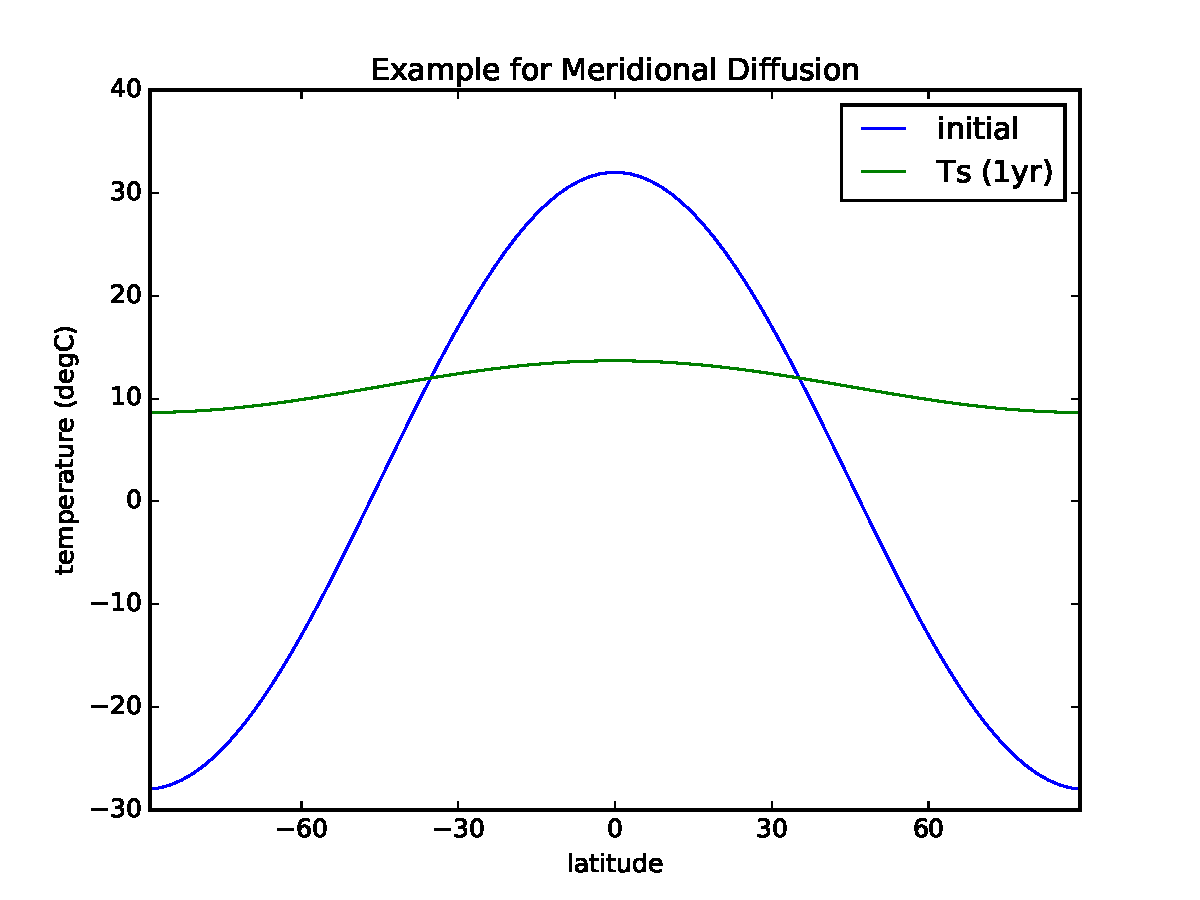
\includegraphics{meridional_diffusion_example.pdf}

\end{description}\end{quote}
\end{quote}

\end{fulllineitems}

\index{\_guess\_diffusion\_axis() (in module climlab.dynamics.diffusion)}

\begin{fulllineitems}
\phantomsection\label{api/climlab.dynamics:climlab.dynamics.diffusion._guess_diffusion_axis}\pysiglinewithargsret{\code{climlab.dynamics.diffusion.}\bfcode{\_guess\_diffusion\_axis}}{\emph{process\_or\_domain}}{}
Input: a process, domain or dictionary of domains.
If there is only one axis with length \textgreater{} 1 in the process or
set of domains, return the name of that axis.
Otherwise raise an error.

\end{fulllineitems}

\index{\_make\_diffusion\_matrix() (in module climlab.dynamics.diffusion)}

\begin{fulllineitems}
\phantomsection\label{api/climlab.dynamics:climlab.dynamics.diffusion._make_diffusion_matrix}\pysiglinewithargsret{\code{climlab.dynamics.diffusion.}\bfcode{\_make\_diffusion\_matrix}}{\emph{K}, \emph{weight1=None}, \emph{weight2=None}}{}
Builds the the diffusion matrix.

\textbf{Function-all argument}
\begin{quote}\begin{description}
\item[{Parameters}] \leavevmode\begin{itemize}
\item {} 
\textbf{\texttt{K}} (\href{http://docs.python.org/2.7/library/array.html\#module-array}{\emph{array}}) -- list of names of diagnostic variables

\item {} 
\textbf{\texttt{weight1}} (\href{http://docs.python.org/2.7/library/array.html\#module-array}{\emph{array}}) -- 

\item {} 
\textbf{\texttt{weight2}} (\href{http://docs.python.org/2.7/library/array.html\#module-array}{\emph{array}}) -- 

\end{itemize}

\end{description}\end{quote}

\textbf{Object attributes}

During method execution following object attribute is modified:
\begin{quote}\begin{description}
\item[{Variables}] \leavevmode
\textbf{\texttt{\_diag\_vars}} (\href{http://docs.python.org/2.7/library/functions.html\#list}{\emph{list}}) -- extended by the list \code{diaglist} given as 
method argument

\end{description}\end{quote}
\begin{description}
\item[{K is array of dimensionless diffusivities at cell boundaries:}] \leavevmode
physical K (length**2 / time) / (delta length)**2 * (delta time)

\end{description}
\begin{gather}
\begin{split}M= \left[ \begin{array}{cccccc}
1+K^* & -K^* & 0 & 0 & ... & 0  \\
-K^* & 1+2K^* & -K^* & 0 & ... & 0 \\
0 & -K^* & 1+2K^* & -K^* &... & 0  \\
  &  & \ddots & \ddots & \ddots & \\
0 & 0 & ... & -K^* & 1+2K^* & -K^* \\
0 & 0 & ... & 0 & -K^* & 1+K^* \\
\end{array} \right]    \end{split}\notag
\end{gather}
\end{fulllineitems}

\index{\_make\_meridional\_diffusion\_matrix() (in module climlab.dynamics.diffusion)}

\begin{fulllineitems}
\phantomsection\label{api/climlab.dynamics:climlab.dynamics.diffusion._make_meridional_diffusion_matrix}\pysiglinewithargsret{\code{climlab.dynamics.diffusion.}\bfcode{\_make\_meridional\_diffusion\_matrix}}{\emph{K}, \emph{lataxis}}{}
\end{fulllineitems}

\index{\_solve\_implicit\_banded() (in module climlab.dynamics.diffusion)}

\begin{fulllineitems}
\phantomsection\label{api/climlab.dynamics:climlab.dynamics.diffusion._solve_implicit_banded}\pysiglinewithargsret{\code{climlab.dynamics.diffusion.}\bfcode{\_solve\_implicit\_banded}}{\emph{current}, \emph{banded\_matrix}}{}
\end{fulllineitems}



\subsubsection{Module contents}
\label{api/climlab.dynamics:module-climlab.dynamics}\label{api/climlab.dynamics:module-contents}\index{climlab.dynamics (module)}

\subsection{climlab.model package}
\label{api/climlab.model:climlab-model-package}\label{api/climlab.model::doc}

\subsubsection{Submodules}
\label{api/climlab.model:submodules}

\subsubsection{climlab.model.column module}
\label{api/climlab.model:module-climlab.model.column}\label{api/climlab.model:climlab-model-column-module}\index{climlab.model.column (module)}
Object-oriented code for radiative-convective models with grey-gas radiation.

Code developed by Brian Rose, University at Albany
\href{mailto:brose@albany.edu}{brose@albany.edu}

Note that the column models by default represent global, time averages.
Thus the insolation is a prescribed constant.

Here is an example to implement seasonal insolation at 45 degrees North
\begin{quote}
\begin{quote}\begin{description}
\item[{Example}] \leavevmode
\begin{Verbatim}[commandchars=\\\{\}]
\PYG{k+kn}{import} \PYG{n+nn}{climlab}

\PYG{c}{\PYGZsh{}  create the column model object}
\PYG{n}{col} \PYG{o}{=} \PYG{n}{climlab}\PYG{o}{.}\PYG{n}{GreyRadiationModel}\PYG{p}{(}\PYG{p}{)}

\PYG{c}{\PYGZsh{}  create a new latitude axis with a single point}
\PYG{n}{lat} \PYG{o}{=} \PYG{n}{climlab}\PYG{o}{.}\PYG{n}{domain}\PYG{o}{.}\PYG{n}{Axis}\PYG{p}{(}\PYG{n}{axis\PYGZus{}type}\PYG{o}{=}\PYG{l+s}{\PYGZsq{}}\PYG{l+s}{lat}\PYG{l+s}{\PYGZsq{}}\PYG{p}{,} \PYG{n}{points}\PYG{o}{=}\PYG{l+m+mf}{45.}\PYG{p}{)}

\PYG{c}{\PYGZsh{}  add this new axis to the surface domain}
\PYG{n}{col}\PYG{o}{.}\PYG{n}{Ts}\PYG{o}{.}\PYG{n}{domain}\PYG{o}{.}\PYG{n}{axes}\PYG{p}{[}\PYG{l+s}{\PYGZsq{}}\PYG{l+s}{lat}\PYG{l+s}{\PYGZsq{}}\PYG{p}{]} \PYG{o}{=} \PYG{n}{lat}

\PYG{c}{\PYGZsh{}  create a new insolation process using this domain}
\PYG{n}{Q} \PYG{o}{=} \PYG{n}{climlab}\PYG{o}{.}\PYG{n}{radiation}\PYG{o}{.}\PYG{n}{insolation}\PYG{o}{.}\PYG{n}{DailyInsolation}\PYG{p}{(}\PYG{n}{domains}\PYG{o}{=}\PYG{n}{col}\PYG{o}{.}\PYG{n}{Ts}\PYG{o}{.}\PYG{n}{domain}\PYG{p}{,} \PYG{o}{*}\PYG{o}{*}\PYG{n}{col}\PYG{o}{.}\PYG{n}{param}\PYG{p}{)}

\PYG{c}{\PYGZsh{}  replace the fixed insolation subprocess in the column model}
\PYG{n}{col}\PYG{o}{.}\PYG{n}{add\PYGZus{}subprocess}\PYG{p}{(}\PYG{l+s}{\PYGZsq{}}\PYG{l+s}{insolation}\PYG{l+s}{\PYGZsq{}}\PYG{p}{,} \PYG{n}{Q}\PYG{p}{)}
\end{Verbatim}

\end{description}\end{quote}
\end{quote}

This model is now a single column with seasonally varying insolation
calculated for 45N.
\index{BandRCModel (class in climlab.model.column)}

\begin{fulllineitems}
\phantomsection\label{api/climlab.model:climlab.model.column.BandRCModel}\pysiglinewithargsret{\strong{class }\code{climlab.model.column.}\bfcode{BandRCModel}}{\emph{**kwargs}}{}
Bases: {\hyperref[api/climlab.model:climlab.model.column.RadiativeConvectiveModel]{\emph{\code{climlab.model.column.RadiativeConvectiveModel}}}}

\end{fulllineitems}

\index{GreyRadiationModel (class in climlab.model.column)}

\begin{fulllineitems}
\phantomsection\label{api/climlab.model:climlab.model.column.GreyRadiationModel}\pysiglinewithargsret{\strong{class }\code{climlab.model.column.}\bfcode{GreyRadiationModel}}{\emph{num\_lev=30}, \emph{num\_lat=1}, \emph{lev=None}, \emph{lat=None}, \emph{water\_depth=1.0}, \emph{albedo\_sfc=0.299}, \emph{timestep=86400.0}, \emph{Q=341.3}, \emph{abs\_coeff=0.0001229}, \emph{**kwargs}}{}
Bases: {\hyperref[api/climlab.process:climlab.process.time_dependent_process.TimeDependentProcess]{\emph{\code{climlab.process.time\_dependent\_process.TimeDependentProcess}}}}
\index{do\_diagnostics() (climlab.model.column.GreyRadiationModel method)}

\begin{fulllineitems}
\phantomsection\label{api/climlab.model:climlab.model.column.GreyRadiationModel.do_diagnostics}\pysiglinewithargsret{\bfcode{do\_diagnostics}}{}{}
Set all the diagnostics from long and shortwave radiation.

\end{fulllineitems}


\end{fulllineitems}

\index{RadiativeConvectiveModel (class in climlab.model.column)}

\begin{fulllineitems}
\phantomsection\label{api/climlab.model:climlab.model.column.RadiativeConvectiveModel}\pysiglinewithargsret{\strong{class }\code{climlab.model.column.}\bfcode{RadiativeConvectiveModel}}{\emph{adj\_lapse\_rate=6.5}, \emph{**kwargs}}{}
Bases: {\hyperref[api/climlab.model:climlab.model.column.GreyRadiationModel]{\emph{\code{climlab.model.column.GreyRadiationModel}}}}

\end{fulllineitems}

\index{compute\_layer\_absorptivity() (in module climlab.model.column)}

\begin{fulllineitems}
\phantomsection\label{api/climlab.model:climlab.model.column.compute_layer_absorptivity}\pysiglinewithargsret{\code{climlab.model.column.}\bfcode{compute\_layer\_absorptivity}}{\emph{abs\_coeff}, \emph{dp}}{}
Compute layer absorptivity from a constant absorption coefficient.

\end{fulllineitems}



\subsubsection{climlab.model.ebm module}
\label{api/climlab.model:climlab-model-ebm-module}\label{api/climlab.model:module-climlab.model.ebm}\index{climlab.model.ebm (module)}\index{EBM (class in climlab.model.ebm)}

\begin{fulllineitems}
\phantomsection\label{api/climlab.model:climlab.model.ebm.EBM}\pysiglinewithargsret{\strong{class }\code{climlab.model.ebm.}\bfcode{EBM}}{\emph{num\_lat=90}, \emph{S0=1365.2}, \emph{A=210.0}, \emph{B=2.0}, \emph{D=0.555}, \emph{water\_depth=10.0}, \emph{Tf=-10.0}, \emph{a0=0.3}, \emph{a2=0.078}, \emph{ai=0.62}, \emph{timestep=350632.51200000005}, \emph{T\_init\_0=12.0}, \emph{T\_init\_P2=-40.0}, \emph{**kwargs}}{}
Bases: {\hyperref[api/climlab.process:climlab.process.energy_budget.EnergyBudget]{\emph{\code{climlab.process.energy\_budget.EnergyBudget}}}}

A parent class for all Energy-Balance-Model classes.

This class sets up a typical EnergyBalance Model with following subprocesses:
\begin{itemize}
\item {} 
Outgoing Longwave Radiation (OLR) parameterization through 
{\hyperref[api/climlab.radiation:climlab.radiation.AplusBT.AplusBT]{\emph{\code{AplusBT}}}}

\item {} 
solar insolation paramterization through 
{\hyperref[api/climlab.radiation:climlab.radiation.insolation.P2Insolation]{\emph{\code{P2Insolation}}}}

\item {} 
albedo parameterization in dependence of temperature through
{\hyperref[api/climlab.surface:climlab.surface.albedo.StepFunctionAlbedo]{\emph{\code{StepFunctionAlbedo}}}}

\item {} 
energy diffusion through 
{\hyperref[api/climlab.dynamics:climlab.dynamics.diffusion.MeridionalDiffusion]{\emph{\code{MeridionalDiffusion}}}}

\end{itemize}

\textbf{Initialization parameters}

An instance of \code{EBM} is initialized with the following 
arguments \emph{(for detailed information see Object attributes below)}:
\begin{quote}\begin{description}
\item[{Parameters}] \leavevmode\begin{itemize}
\item {} 
\textbf{\texttt{num\_lat}} (\href{http://docs.python.org/2.7/library/functions.html\#int}{\emph{int}}) -- 
number of equally spaced points for the 
latitue grid. Used for domain intialization of
{\hyperref[api/climlab.domain:climlab.domain.domain.zonal_mean_surface]{\emph{\code{zonal\_mean\_surface}}}}
\begin{itemize}
\item {} 
default value: \code{90}

\end{itemize}


\item {} 
\textbf{\texttt{S0}} (\href{http://docs.python.org/2.7/library/functions.html\#float}{\emph{float}}) -- 
solar constant
\begin{itemize}
\item {} 
unit: \(\frac{\textrm{W}}{\textrm{m}^2}\)

\item {} 
default value: \code{1365.2}

\end{itemize}


\item {} 
\textbf{\texttt{A}} (\href{http://docs.python.org/2.7/library/functions.html\#float}{\emph{float}}) -- 
parameter for linear OLR parameterization
{\hyperref[api/climlab.radiation:climlab.radiation.AplusBT.AplusBT]{\emph{\code{AplusBT}}}}
\begin{itemize}
\item {} 
unit: \(\frac{\textrm{W}}{\textrm{m}^2}\)

\item {} 
default value: \code{210.0}

\end{itemize}


\item {} 
\textbf{\texttt{B}} (\href{http://docs.python.org/2.7/library/functions.html\#float}{\emph{float}}) -- 
parameter for linear OLR parameterization
{\hyperref[api/climlab.radiation:climlab.radiation.AplusBT.AplusBT]{\emph{\code{AplusBT}}}}
\begin{itemize}
\item {} 
unit: \(\frac{\textrm{W}}{\textrm{m}^2 \ ^{\circ} \textrm{C}}\)

\item {} 
default value: \code{2.0}

\end{itemize}


\item {} 
\textbf{\texttt{D}} (\href{http://docs.python.org/2.7/library/functions.html\#float}{\emph{float}}) -- 
diffusion parameter for Meridional Energy Diffusion
{\hyperref[api/climlab.dynamics:climlab.dynamics.diffusion.MeridionalDiffusion]{\emph{\code{MeridionalDiffusion}}}}
\begin{itemize}
\item {} 
unit: \(\frac{\textrm{W}}{\textrm{m}^2 \ ^{\circ} \textrm{C}}\)

\item {} 
default value: \code{0.555}

\end{itemize}


\item {} 
\textbf{\texttt{water\_depth}} (\href{http://docs.python.org/2.7/library/functions.html\#float}{\emph{float}}) -- 
depth of {\hyperref[api/climlab.domain:climlab.domain.domain.zonal_mean_surface]{\emph{\code{zonal\_mean\_surface}}}}
domain, which the heat capacity is dependent on
\begin{itemize}
\item {} 
unit: meters

\item {} 
default value: \code{10.0}

\end{itemize}


\item {} 
\textbf{\texttt{Tf}} (\href{http://docs.python.org/2.7/library/functions.html\#float}{\emph{float}}) -- 
freezing temperature
\begin{itemize}
\item {} 
unit \(^{\circ} \textrm{C}\)

\item {} 
default value: \code{-10.0}

\end{itemize}


\item {} 
\textbf{\texttt{a0}} (\href{http://docs.python.org/2.7/library/functions.html\#float}{\emph{float}}) -- 
base value for planetary albedo parameterization
{\hyperref[api/climlab.surface:climlab.surface.albedo.StepFunctionAlbedo]{\emph{\code{StepFunctionAlbedo}}}}
\begin{itemize}
\item {} 
default value: \code{0.3}

\end{itemize}


\item {} 
\textbf{\texttt{a2}} (\href{http://docs.python.org/2.7/library/functions.html\#float}{\emph{float}}) -- 
parabolic value for planetary  albedo parameterization
{\hyperref[api/climlab.surface:climlab.surface.albedo.StepFunctionAlbedo]{\emph{\code{StepFunctionAlbedo}}}}
\begin{itemize}
\item {} 
default value: \code{0.078}

\end{itemize}


\item {} 
\textbf{\texttt{ai}} (\href{http://docs.python.org/2.7/library/functions.html\#float}{\emph{float}}) -- 
value for ice albedo paramerization in
{\hyperref[api/climlab.surface:climlab.surface.albedo.StepFunctionAlbedo]{\emph{\code{StepFunctionAlbedo}}}}
\begin{itemize}
\item {} 
default value: \code{0.62}

\end{itemize}


\item {} 
\textbf{\texttt{timestep}} (\href{http://docs.python.org/2.7/library/functions.html\#float}{\emph{float}}) -- specifies the EBM's timestep

\item {} 
\textbf{\texttt{T\_init\_0}} (\href{http://docs.python.org/2.7/library/functions.html\#float}{\emph{float}}) -- 
base value for initial temperature
\begin{itemize}
\item {} 
unit \(^{\circ} \textrm{C}\)

\item {} 
default value: \code{12}

\end{itemize}


\item {} 
\textbf{\texttt{T\_init\_P2}} (\href{http://docs.python.org/2.7/library/functions.html\#float}{\emph{float}}) -- 
2nd Legendre polynomial value for initial temperature
\begin{itemize}
\item {} 
default value: \code{40}

\end{itemize}


\end{itemize}

\end{description}\end{quote}

\textbf{Object attributes}

Additional to the parent class {\hyperref[api/climlab.process:climlab.process.energy_budget.EnergyBudget]{\emph{\code{EnergyBudget}}}}
following object attributes are generated and updated during initialization:
\begin{quote}\begin{description}
\item[{Variables}] \leavevmode\begin{itemize}
\item {} 
\textbf{\texttt{param}} (\href{http://docs.python.org/2.7/library/stdtypes.html\#dict}{\emph{dict}}) -- The parameter dictionary is updated with a couple 
of the initatilzation input arguments, namely
\code{'S0'}, \code{'A'}, \code{'B'}, \code{'D'}, \code{'Tf'}, 
\code{'water\_depth'}, \code{'a0'}, \code{'a2'} and \code{'ai'}.

\item {} 
\textbf{\texttt{domains}} (\href{http://docs.python.org/2.7/library/stdtypes.html\#dict}{\emph{dict}}) -- If the object's \code{domains} and the \code{state} 
dictionaries are empty during initialization 
a domain \code{sfc} is created through 
{\hyperref[api/climlab.domain:climlab.domain.domain.zonal_mean_surface]{\emph{\code{zonal\_mean\_surface()}}}}.
In the meantime the object's \code{domains} and 
\code{state} dictionaries are updated.

\item {} 
\href{http://docs.python.org/2.7/library/subprocess.html\#module-subprocess}{\textbf{\texttt{subprocess}}} (\href{http://docs.python.org/2.7/library/stdtypes.html\#dict}{\emph{dict}}) -- Several subprocesses are created (see above) 
through calling 
{\hyperref[api/climlab.process:climlab.process.process.Process.add_subprocess]{\emph{\code{add\_subprocess()}}}}
and therefore the subprocess dictionary is updated.

\item {} 
\textbf{\texttt{topdown}} (\href{http://docs.python.org/2.7/library/functions.html\#bool}{\emph{bool}}) -- is set to \code{False} to call subprocess compute 
methods first.
See also 
{\hyperref[api/climlab.process:climlab.process.time_dependent_process.TimeDependentProcess]{\emph{\code{TimeDependentProcess}}}}.

\item {} 
\textbf{\texttt{\_diag\_vars}} (\href{http://docs.python.org/2.7/library/functions.html\#list}{\emph{list}}) -- is updated with \code{{[}'OLR','ASR','net\_radiation','icelat'{]}}
through {\hyperref[api/climlab.process:climlab.process.process.Process.add_diagnostics]{\emph{\code{add\_diagnostics()}}}}.

\end{itemize}

\end{description}\end{quote}
\index{diffusive\_heat\_transport() (climlab.model.ebm.EBM method)}

\begin{fulllineitems}
\phantomsection\label{api/climlab.model:climlab.model.ebm.EBM.diffusive_heat_transport}\pysiglinewithargsret{\bfcode{diffusive\_heat\_transport}}{}{}
Compute instantaneous diffusive heat transport in unit \(\textrm{PW}\)
on the staggered grid (bounds) through calculating:
\begin{gather}
\begin{split}H(\varphi) = - 2 \pi R^2 cos(\varphi) D \frac{dT}{d\varphi}
            \approx - 2 \pi R^2 cos(\varphi) D \frac{\Delta T}{\Delta \varphi}\end{split}\notag
\end{gather}\begin{quote}\begin{description}
\item[{Return type}] \leavevmode
array of size \code{np.size(self.lat\_bounds)}

\end{description}\end{quote}

\end{fulllineitems}

\index{global\_mean\_temperature() (climlab.model.ebm.EBM method)}

\begin{fulllineitems}
\phantomsection\label{api/climlab.model:climlab.model.ebm.EBM.global_mean_temperature}\pysiglinewithargsret{\bfcode{global\_mean\_temperature}}{}{}
Convenience method to compute global mean surface temperature.

Calls {\hyperref[api/climlab.domain:climlab.domain.field.global_mean]{\emph{\code{global\_mean()}}}} method which
for the object attriute \code{Ts} which calculates the latitude weighted
global mean of a field.

\end{fulllineitems}

\index{heat\_transport() (climlab.model.ebm.EBM method)}

\begin{fulllineitems}
\phantomsection\label{api/climlab.model:climlab.model.ebm.EBM.heat_transport}\pysiglinewithargsret{\bfcode{heat\_transport}}{}{}
Returns instantaneous heat transport in unit \(\textrm{PW}\)
on the staggered grid (bounds) through calling {\hyperref[api/climlab.model:climlab.model.ebm.EBM.diffusive_heat_transport]{\emph{\code{diffusive\_heat\_transport()}}}}.

\end{fulllineitems}

\index{heat\_transport\_convergence() (climlab.model.ebm.EBM method)}

\begin{fulllineitems}
\phantomsection\label{api/climlab.model:climlab.model.ebm.EBM.heat_transport_convergence}\pysiglinewithargsret{\bfcode{heat\_transport\_convergence}}{}{}
Returns instantaneous convergence of heat transport.
\begin{gather}
\begin{split}h(\varphi) = - \frac{1}{2 \pi R^2 cos(\varphi)} \frac{dH}{d\varphi} 
            \approx - \frac{1}{2 \pi R^2 cos(\varphi)} \frac{\Delta H}{\Delta \varphi} \end{split}\notag
\end{gather}
h is the \emph{dynamical heating rate} in unit \(\textrm{W}/ \textrm{m}^2\)
which is the convergence of energy transport into each latitude band,
namely the difference between what's coming in and what's going out.

\end{fulllineitems}

\index{inferred\_heat\_transport() (climlab.model.ebm.EBM method)}

\begin{fulllineitems}
\phantomsection\label{api/climlab.model:climlab.model.ebm.EBM.inferred_heat_transport}\pysiglinewithargsret{\bfcode{inferred\_heat\_transport}}{}{}
Calculates the inferred heat transport by integrating the TOA 
energy imbalance from pole to pole.

The method is calculating
\begin{gather}
\begin{split}H(\varphi) = 2 \pi R^2 \int_{-\pi/2}^{\varphi} cos\phi \ R_{TOA} d\phi\end{split}\notag
\end{gather}
where \(R_{TOA}\) is the net radiation at top of atmosphere.
\begin{quote}\begin{description}
\item[{Returns}] \leavevmode
total heat transport on the latitude grid in unit \(\textrm{PW}\)

\item[{Return type}] \leavevmode
array of size \code{np.size(self.lat\_lat)}

\end{description}\end{quote}

\end{fulllineitems}


\end{fulllineitems}

\index{EBM\_annual (class in climlab.model.ebm)}

\begin{fulllineitems}
\phantomsection\label{api/climlab.model:climlab.model.ebm.EBM_annual}\pysiglinewithargsret{\strong{class }\code{climlab.model.ebm.}\bfcode{EBM\_annual}}{\emph{**kwargs}}{}
Bases: {\hyperref[api/climlab.model:climlab.model.ebm.EBM_seasonal]{\emph{\code{climlab.model.ebm.EBM\_seasonal}}}}

A class that implements Energy Balance Models with annual mean insolation.

The annual solar distribution is calculated through averaging the 
{\hyperref[api/climlab.radiation:climlab.radiation.insolation.DailyInsolation]{\emph{\code{DailyInsolation}}}} over time 
ehich has been used in used in the parent class
{\hyperref[api/climlab.model:climlab.model.ebm.EBM_seasonal]{\emph{\code{EBM\_seasonal}}}}. That is done by the subprocess
{\hyperref[api/climlab.radiation:climlab.radiation.insolation.AnnualMeanInsolation]{\emph{\code{AnnualMeanInsolation}}}} which is
more realistic than the {\hyperref[api/climlab.radiation:climlab.radiation.insolation.P2Insolation]{\emph{\code{P2Insolation}}}}
module used in the classical {\hyperref[api/climlab.model:climlab.model.ebm.EBM]{\emph{\code{EBM}}}} class.

According to the parent class {\hyperref[api/climlab.model:climlab.model.ebm.EBM_seasonal]{\emph{\code{EBM\_seasonal}}}}
the model will not have an albedo feedback, if albedo ice parameter
\code{'ai'} is not given. For details see there.

\textbf{Object attributes}

Following object attributes are updated during initialization:
\begin{quote}\begin{description}
\item[{Variables}] \leavevmode
\href{http://docs.python.org/2.7/library/subprocess.html\#module-subprocess}{\textbf{\texttt{subprocess}}} (\href{http://docs.python.org/2.7/library/stdtypes.html\#dict}{\emph{dict}}) -- suprocess \code{'insolation'} is overwritten by
{\hyperref[api/climlab.radiation:climlab.radiation.insolation.AnnualMeanInsolation]{\emph{\code{AnnualMeanInsolation}}}}

\end{description}\end{quote}

\end{fulllineitems}

\index{EBM\_seasonal (class in climlab.model.ebm)}

\begin{fulllineitems}
\phantomsection\label{api/climlab.model:climlab.model.ebm.EBM_seasonal}\pysiglinewithargsret{\strong{class }\code{climlab.model.ebm.}\bfcode{EBM\_seasonal}}{\emph{a0=0.33}, \emph{a2=0.25}, \emph{ai=None}, \emph{**kwargs}}{}
Bases: {\hyperref[api/climlab.model:climlab.model.ebm.EBM]{\emph{\code{climlab.model.ebm.EBM}}}}

A class that implements Energy Balance Models with realistic 
daily insolation.

This class is inherited from the general {\hyperref[api/climlab.model:climlab.model.ebm.EBM]{\emph{\code{EBM}}}}
class and uses the insolation subprocess 
{\hyperref[api/climlab.radiation:climlab.radiation.insolation.DailyInsolation]{\emph{\code{DailyInsolation}}}} instead of 
{\hyperref[api/climlab.radiation:climlab.radiation.insolation.P2Insolation]{\emph{\code{P2Insolation}}}} to compute a
realisitc distribution of solar radiation on a daily basis.

If argument for ice albedo \code{'ai'} is not given, the model will not 
have an albedo feedback.

An instance of \code{EBM\_seasonal} is initialized with the following 
arguments:
\begin{quote}\begin{description}
\item[{Parameters}] \leavevmode\begin{itemize}
\item {} 
\textbf{\texttt{a0}} (\href{http://docs.python.org/2.7/library/functions.html\#float}{\emph{float}}) -- 
base value for planetary albedo parameterization
{\hyperref[api/climlab.surface:climlab.surface.albedo.StepFunctionAlbedo]{\emph{\code{StepFunctionAlbedo}}}}
\begin{itemize}
\item {} 
default value: \code{0.33}

\end{itemize}


\item {} 
\textbf{\texttt{a2}} (\href{http://docs.python.org/2.7/library/functions.html\#float}{\emph{float}}) -- 
parabolic value for planetary  albedo parameterization
{\hyperref[api/climlab.surface:climlab.surface.albedo.StepFunctionAlbedo]{\emph{\code{StepFunctionAlbedo}}}}
\begin{itemize}
\item {} 
default value: \code{0.25}

\end{itemize}


\item {} 
\textbf{\texttt{ai}} (\href{http://docs.python.org/2.7/library/functions.html\#float}{\emph{float}}) -- 
value for ice albedo paramerization in
{\hyperref[api/climlab.surface:climlab.surface.albedo.StepFunctionAlbedo]{\emph{\code{StepFunctionAlbedo}}}}
\begin{itemize}
\item {} 
default value: \code{None}

\end{itemize}


\end{itemize}

\end{description}\end{quote}

\textbf{Object attributes}

Following object attributes are updated during initialization:
\begin{quote}\begin{description}
\item[{Variables}] \leavevmode\begin{itemize}
\item {} 
\textbf{\texttt{param}} (\href{http://docs.python.org/2.7/library/stdtypes.html\#dict}{\emph{dict}}) -- The parameter dictionary is updated with 
\code{'a0'} and \code{'a2'}.

\item {} 
\href{http://docs.python.org/2.7/library/subprocess.html\#module-subprocess}{\textbf{\texttt{subprocess}}} (\href{http://docs.python.org/2.7/library/stdtypes.html\#dict}{\emph{dict}}) -- suprocess \code{'insolation'} is overwritten by
{\hyperref[api/climlab.radiation:climlab.radiation.insolation.DailyInsolation]{\emph{\code{DailyInsolation}}}}.

\end{itemize}

\end{description}\end{quote}

\emph{if} \code{'ai'} \emph{is not given}:
\begin{quote}\begin{description}
\item[{Variables}] \leavevmode\begin{itemize}
\item {} 
\textbf{\texttt{param}} (\href{http://docs.python.org/2.7/library/stdtypes.html\#dict}{\emph{dict}}) -- \code{'ai'} and \code{'Tf'} are removed from the 
parameter dictionary (initialized by parent class
{\hyperref[api/climlab.model:climlab.model.ebm.EBM]{\emph{\code{EBM}}}})

\item {} 
\href{http://docs.python.org/2.7/library/subprocess.html\#module-subprocess}{\textbf{\texttt{subprocess}}} (\href{http://docs.python.org/2.7/library/stdtypes.html\#dict}{\emph{dict}}) -- suprocess \code{'albedo'} is overwritten by
{\hyperref[api/climlab.surface:climlab.surface.albedo.P2Albedo]{\emph{\code{P2Albedo}}}}.

\end{itemize}

\end{description}\end{quote}

\emph{if} \code{'ai'} \emph{is given}:
\begin{quote}\begin{description}
\item[{Variables}] \leavevmode\begin{itemize}
\item {} 
\textbf{\texttt{param}} (\href{http://docs.python.org/2.7/library/stdtypes.html\#dict}{\emph{dict}}) -- The parameter dictionary is updated with
\code{'ai'}.

\item {} 
\href{http://docs.python.org/2.7/library/subprocess.html\#module-subprocess}{\textbf{\texttt{subprocess}}} (\href{http://docs.python.org/2.7/library/stdtypes.html\#dict}{\emph{dict}}) -- suprocess \code{'albedo'} is overwritten by
{\hyperref[api/climlab.surface:climlab.surface.albedo.StepFunctionAlbedo]{\emph{\code{StepFunctionAlbedo}}}} 
(which basically has been there before but now is 
updated with the new albedo parameter values).

\end{itemize}

\end{description}\end{quote}

\end{fulllineitems}



\subsubsection{climlab.model.stommelbox module}
\label{api/climlab.model:climlab-model-stommelbox-module}

\subsubsection{Module contents}
\label{api/climlab.model:module-climlab.model}\label{api/climlab.model:module-contents}\index{climlab.model (module)}

\subsection{climlab.process package}
\label{api/climlab.process:climlab-process-package}\label{api/climlab.process::doc}

\subsubsection{Module contents}
\label{api/climlab.process:module-climlab.process}\label{api/climlab.process:module-contents}\index{climlab.process (module)}
module content test


\subsubsection{Submodules}
\label{api/climlab.process:submodules}

\subsubsection{climlab.process.diagnostic module}
\label{api/climlab.process:module-climlab.process.diagnostic}\label{api/climlab.process:climlab-process-diagnostic-module}\index{climlab.process.diagnostic (module)}\index{DiagnosticProcess (class in climlab.process.diagnostic)}

\begin{fulllineitems}
\phantomsection\label{api/climlab.process:climlab.process.diagnostic.DiagnosticProcess}\pysiglinewithargsret{\strong{class }\code{climlab.process.diagnostic.}\bfcode{DiagnosticProcess}}{\emph{**kwargs}}{}
Bases: {\hyperref[api/climlab.process:climlab.process.time_dependent_process.TimeDependentProcess]{\emph{\code{climlab.process.time\_dependent\_process.TimeDependentProcess}}}}

A parent class for all processes that are strictly diagnostic, namely
no time dependence.

During initialization following attribute is set:
\begin{quote}\begin{description}
\item[{Variables}] \leavevmode
\textbf{\texttt{time\_type}} (\href{http://docs.python.org/2.7/library/functions.html\#str}{\emph{str}}) -- is set to \code{'diagnostic'}

\end{description}\end{quote}

\end{fulllineitems}



\subsubsection{climlab.process.energy\_budget module}
\label{api/climlab.process:module-climlab.process.energy_budget}\label{api/climlab.process:climlab-process-energy-budget-module}\index{climlab.process.energy\_budget (module)}\index{EnergyBudget (class in climlab.process.energy\_budget)}

\begin{fulllineitems}
\phantomsection\label{api/climlab.process:climlab.process.energy_budget.EnergyBudget}\pysiglinewithargsret{\strong{class }\code{climlab.process.energy\_budget.}\bfcode{EnergyBudget}}{\emph{**kwargs}}{}
Bases: {\hyperref[api/climlab.process:climlab.process.time_dependent_process.TimeDependentProcess]{\emph{\code{climlab.process.time\_dependent\_process.TimeDependentProcess}}}}

A parent class for explicit energy budget processes.

This class solves equations that include a heat capacitiy term like
\(C \frac{dT}{dt} = \textrm{flux convergence}\)

In an Energy Balance Model with model state \(T\) this equation 
will look like this:
\begin{gather}
\begin{split}C \frac{dT}{dt} = R\downarrow - R\uparrow - H  \end{split}\notag\\\begin{split}\frac{dT}{dt} = \frac{R\downarrow}{C} - \frac{R\uparrow}{C} - \frac{H}{C}\end{split}\notag
\end{gather}
Every EnergyBudget object has a \code{heating\_rate} dictionary with items 
corresponding to each state variable. The heating rate accounts the actual 
heating of a subprocess, namely the contribution to the energy budget 
of \(R\downarrow, R\uparrow\) and \(H\) in this case.
The temperature tendencies for each subprocess are then calculated 
through dividing the heating rate by the heat capacitiy \(C\).

\textbf{Initialization parameters}

An instance of \code{EnergyBudget} is initialized with the forwarded 
keyword arguments \code{**kwargs} of the corresponding children classes.

\textbf{Object attributes}

Additional to the parent class 
\code{TimeDependentProcess}
following object attributes are generated or modified during initialization:
\begin{quote}\begin{description}
\item[{Variables}] \leavevmode\begin{itemize}
\item {} 
\textbf{\texttt{time\_type}} (\href{http://docs.python.org/2.7/library/functions.html\#str}{\emph{str}}) -- is set to \code{'explicit'}

\item {} 
\textbf{\texttt{heating\_rate}} (\href{http://docs.python.org/2.7/library/stdtypes.html\#dict}{\emph{dict}}) -- energy share for given subprocess in unit 
\(\textrm{W}/ \textrm{m}^2\) stored 
in a dictionary sorted by model states

\end{itemize}

\end{description}\end{quote}

\end{fulllineitems}

\index{ExternalEnergySource (class in climlab.process.energy\_budget)}

\begin{fulllineitems}
\phantomsection\label{api/climlab.process:climlab.process.energy_budget.ExternalEnergySource}\pysiglinewithargsret{\strong{class }\code{climlab.process.energy\_budget.}\bfcode{ExternalEnergySource}}{\emph{**kwargs}}{}
Bases: {\hyperref[api/climlab.process:climlab.process.energy_budget.EnergyBudget]{\emph{\code{climlab.process.energy\_budget.EnergyBudget}}}}

A fixed energy source or sink to be specified by the user.

\textbf{Initialization parameters}

An instance of \code{ExternalEnergySource} is initialized with the forwarded 
keyword arguments \code{**kwargs} of hypthetical corresponding children classes
(which are not existing in this case).

\textbf{Object attributes}

Additional to the parent class {\hyperref[api/climlab.process:climlab.process.energy_budget.EnergyBudget]{\emph{\code{EnergyBudget}}}}
the following object attribute is modified during initialization:
\begin{quote}\begin{description}
\item[{Variables}] \leavevmode
\textbf{\texttt{heating\_rate}} (\href{http://docs.python.org/2.7/library/stdtypes.html\#dict}{\emph{dict}}) -- energy share dictionary for this subprocess
is set to zero for every model state.

\end{description}\end{quote}

After initialization the user should modify the fields in the 
\code{heating\_rate} dictionary, which contain heating rates in 
unit \(\textrm{W}/ \textrm{m}^2\) for all state variables.

\end{fulllineitems}



\subsubsection{climlab.process.implicit module}
\label{api/climlab.process:climlab-process-implicit-module}\label{api/climlab.process:module-climlab.process.implicit}\index{climlab.process.implicit (module)}\index{ImplicitProcess (class in climlab.process.implicit)}

\begin{fulllineitems}
\phantomsection\label{api/climlab.process:climlab.process.implicit.ImplicitProcess}\pysiglinewithargsret{\strong{class }\code{climlab.process.implicit.}\bfcode{ImplicitProcess}}{\emph{**kwargs}}{}
Bases: {\hyperref[api/climlab.process:climlab.process.time_dependent_process.TimeDependentProcess]{\emph{\code{climlab.process.time\_dependent\_process.TimeDependentProcess}}}}

A parent class for modules that use implicit time discretization.

During initialization following attributes are intitialized:
\begin{quote}\begin{description}
\item[{Variables}] \leavevmode\begin{itemize}
\item {} 
\textbf{\texttt{time\_type}} (\href{http://docs.python.org/2.7/library/functions.html\#str}{\emph{str}}) -- is set to \code{'implicit'}

\item {} 
\textbf{\texttt{adjustment}} (\href{http://docs.python.org/2.7/library/stdtypes.html\#dict}{\emph{dict}}) -- the model state adjustments due to this implicit 
subprocess

\end{itemize}

\end{description}\end{quote}

Calculating the model state adjustments through solving the matrix problem 
already includes the multiplication with the timestep. The adjustment is
divided by the timestep to calculate the implicit subprocess tendencies,
which can be handeled by the 
{\hyperref[api/climlab.process:climlab.process.time_dependent_process.TimeDependentProcess.compute]{\emph{\code{compute()}}}}
method of the parent 
{\hyperref[api/climlab.process:climlab.process.time_dependent_process.TimeDependentProcess]{\emph{\code{TimeDependentProcess}}}} class.

\end{fulllineitems}



\subsubsection{climlab.process.process module}
\label{api/climlab.process:climlab-process-process-module}\label{api/climlab.process:module-climlab.process.process}\index{climlab.process.process (module)}
Principles of the new \emph{climlab} API design:
\begin{itemize}
\item {} 
\emph{climlab.Process} object has several iterable dictionaries of named,
gridded variables:
\begin{quote}
\begin{itemize}
\item {} 
\emph{process.state}
\begin{itemize}
\item {} 
state variables, usually time-dependent

\end{itemize}

\end{itemize}
\begin{itemize}
\item {} \begin{description}
\item[{\emph{process.input}}] \leavevmode\begin{itemize}
\item {} 
boundary conditions and other gridded quantities independent of the

\end{itemize}

\emph{process}
- often set by a parent \emph{process}

\end{description}

\item {} 
\emph{process.param}  (which are basically just scalar \emph{input})

\item {} \begin{description}
\item[{\emph{process.tendencies}}] \leavevmode\begin{itemize}
\item {} 
iterable \emph{dict} of time-tendencies (d/dt) for each state variable

\end{itemize}

\end{description}

\item {} \begin{description}
\item[{\emph{process.diagnostics}}] \leavevmode\begin{itemize}
\item {} 
any quantity derived from current state

\end{itemize}

\end{description}

\end{itemize}
\end{quote}

\end{itemize}
\begin{itemize}
\item {} 
The \emph{process} is fully described by contents of \emph{state}, \emph{input} and \emph{param}

\end{itemize}

dictionaries. \emph{tendencies} and \emph{diagnostics} are always computable from current
state.
- \emph{climlab} will remain (as much as possible) agnostic about the data formats
\begin{quote}
\begin{itemize}
\item {} 
Variables within the dictionaries will behave as \emph{numpy.ndarray} objects

\item {} 
Grid information and other domain details accessible as attributes

\end{itemize}
\begin{description}
\item[{of each variable}] \leavevmode\begin{itemize}
\item {} 
e.g. Tatm.lat

\item {} 
Shortcuts like \emph{process.lat} will work where these are unambiguous

\end{itemize}

\end{description}
\end{quote}
\begin{itemize}
\item {} \begin{description}
\item[{Many variables will be accessible as process attributes \emph{process.name}}] \leavevmode\begin{itemize}
\item {} 
this restricts to unique field names in the above dictionaries

\end{itemize}

\end{description}

\item {} \begin{description}
\item[{There may be other dictionaries that do have name conflicts}] \leavevmode\begin{itemize}
\item {} 
e.g. dictionary of tendencies, with same keys as \emph{process.state}

\item {} 
These will \emph{not} be accessible as \emph{process.name}

\item {} 
but \emph{will} be accessible as \emph{process.dict\_name.name}

\end{itemize}

(as well as regular dict interface)

\end{description}

\item {} 
There will be a dictionary of named subprocesses \emph{process.subprocess}

\item {} 
Each item in subprocess dict will itself be a \emph{climlab.Process} object

\item {} 
For convenience with interactive work, each subprocess should be accessible

\end{itemize}

as \emph{process.subprocess.name} as well as \emph{process.subprocess{[}'name'{]}}
- \emph{process.compute()} is a method that computes tendencies (d/dt)
\begin{itemize}
\item {} 
returns a dictionary of tendencies for all state variables

\item {} 
keys for this dictionary are same as keys of state dictionary

\item {} 
tendency dictionary is the total tendency including all subprocesses

\item {} 
method only computes d/dt, does not apply changes

\item {} \begin{description}
\item[{thus method is relatively independent of numerical scheme}] \leavevmode\begin{itemize}
\item {} 
may need to make exception for implicit scheme?

\end{itemize}

\end{description}

\item {} \begin{description}
\item[{method \emph{will} update variables in \emph{process.diagnostic}}] \leavevmode\begin{itemize}
\item {} 
will also \emph{gather all diagnostics} from \emph{subprocesses}

\end{itemize}

\end{description}

\end{itemize}
\begin{itemize}
\item {} \begin{description}
\item[{\emph{process.step\_forward()} updates the state variables}] \leavevmode\begin{itemize}
\item {} 
calls \emph{process.compute()} to get current tendencies

\item {} 
implements a particular time-stepping scheme

\item {} 
user interface is agnostic about numerical scheme

\end{itemize}

\end{description}

\item {} \begin{description}
\item[{\emph{process.integrate\_years()} etc will automate time-stepping}] \leavevmode\begin{itemize}
\item {} 
also computation of time-average diagnostics.

\end{itemize}

\end{description}

\item {} 
Every \emph{subprocess} should work independently of its parent \emph{process} given

\end{itemize}
\begin{description}
\item[{appropriate \emph{input}.}] \leavevmode\begin{itemize}
\item {} 
investigating an individual \emph{process} (possibly with its own

\end{itemize}
\begin{description}
\item[{\emph{subprocesses}) isolated from its parent needs to be as simple as doing:}] \leavevmode\begin{itemize}
\item {} 
\emph{newproc = climlab.process\_like(procname.subprocess{[}'subprocname'{]})}

\item {} 
\emph{newproc.compute()}

\item {} 
anything in the \emph{input} dictionary of \emph{subprocname} will remain fixed

\end{itemize}

\end{description}

\end{description}

To do:
- use OrderedDict to hold the subprocess dictionary
\begin{itemize}
\item {} 
order of execution can then be controled by position in dictionary

\end{itemize}
\index{Process (class in climlab.process.process)}

\begin{fulllineitems}
\phantomsection\label{api/climlab.process:climlab.process.process.Process}\pysiglinewithargsret{\strong{class }\code{climlab.process.process.}\bfcode{Process}}{\emph{state=None}, \emph{domains=None}, \emph{subprocess=None}, \emph{lat=None}, \emph{lev=None}, \emph{num\_lat=None}, \emph{num\_levels=None}, \emph{input=None}, \emph{**kwargs}}{}
Bases: \href{http://docs.python.org/2.7/library/functions.html\#object}{\code{object}}

A generic parent class for all climlab process objects.

Every process object has a set of state variables on a spatial grid.

\textbf{Initialization parameters}

An instance of \code{Process} is initialized with the following 
arguments \emph{(for detailed information see Object attributes below)}:
\begin{quote}\begin{description}
\item[{Parameters}] \leavevmode\begin{itemize}
\item {} 
\textbf{\texttt{state}} ({\hyperref[api/climlab.domain:climlab.domain.field.Field]{\emph{\emph{Field}}}}) -- spatial state variable for the process. 
Set to \code{None} if not specified.

\item {} 
\textbf{\texttt{domains}} ({\hyperref[api/climlab.domain:climlab.domain.domain._Domain]{\emph{\code{\_Domain}}}} or dict of 
{\hyperref[api/climlab.domain:climlab.domain.domain._Domain]{\emph{\code{\_Domain}}}}) -- domain(s) for the process

\item {} 
\textbf{\texttt{subprocess}} ({\hyperref[api/climlab.process:climlab.process.process.Process]{\emph{\code{Process}}}} or dict of 
{\hyperref[api/climlab.process:climlab.process.process.Process]{\emph{\code{Process}}}}) -- subprocess(es) of the process

\item {} 
\textbf{\texttt{lat}} -- 

\item {} 
\textbf{\texttt{lev}} -- 

\item {} 
\textbf{\texttt{num\_lat}} -- 

\item {} 
\textbf{\texttt{num\_levels}} -- 

\item {} 
\textbf{\texttt{input}} (\href{http://docs.python.org/2.7/library/stdtypes.html\#dict}{\emph{dict}}) -- collection of input quantities

\end{itemize}

\end{description}\end{quote}

\textbf{Object attributes}

Additional to the parent class {\hyperref[api/climlab.process:climlab.process.process.Process]{\emph{\code{Process}}}}
following object attributes are generated during initialization:
\begin{quote}\begin{description}
\item[{Variables}] \leavevmode\begin{itemize}
\item {} 
\textbf{\texttt{domains}} (\href{http://docs.python.org/2.7/library/stdtypes.html\#dict}{\emph{dict}}) -- dictionary of process :class:{\color{red}\bfseries{}{}`}\textasciitilde{}climlab.domain.domain.\_Domain{}`s

\item {} 
\textbf{\texttt{state}} (\href{http://docs.python.org/2.7/library/stdtypes.html\#dict}{\emph{dict}}) -- dictionary of process states 
(of type {\hyperref[api/climlab.domain:climlab.domain.field.Field]{\emph{\code{Field}}}})

\item {} 
\textbf{\texttt{param}} (\href{http://docs.python.org/2.7/library/stdtypes.html\#dict}{\emph{dict}}) -- dictionary of model parameters which are given
through \code{**kwargs}

\item {} 
\textbf{\texttt{\_diag\_vars}} (\href{http://docs.python.org/2.7/library/stdtypes.html\#frozenset}{\emph{frozenset}}) -- basically a list of names of diagnostic variables

\item {} 
\textbf{\texttt{\_input\_vars}} (\href{http://docs.python.org/2.7/library/stdtypes.html\#dict}{\emph{dict}}) -- collection of input quantities like boundary conditions
and other gridded quantities

\item {} 
\textbf{\texttt{creation\_date}} (\href{http://docs.python.org/2.7/library/functions.html\#str}{\emph{str}}) -- date and time when process was created

\item {} 
\href{http://docs.python.org/2.7/library/subprocess.html\#module-subprocess}{\textbf{\texttt{subprocess}}} (dict of {\hyperref[api/climlab.process:climlab.process.process.Process]{\emph{\code{Process}}}}) -- dictionary of suprocesses of the process

\end{itemize}

\end{description}\end{quote}
\index{add\_diagnostics() (climlab.process.process.Process method)}

\begin{fulllineitems}
\phantomsection\label{api/climlab.process:climlab.process.process.Process.add_diagnostics}\pysiglinewithargsret{\bfcode{add\_diagnostics}}{\emph{diaglist}}{}
Updates the process's list of diagnostics.

\textbf{Function-call argument}
\begin{quote}\begin{description}
\item[{Parameters}] \leavevmode
\textbf{\texttt{diaglist}} (\href{http://docs.python.org/2.7/library/functions.html\#list}{\emph{list}}) -- list of names of diagnostic variables

\end{description}\end{quote}

\textbf{Object attributes}

During method execution following object attribute is modified:
\begin{quote}\begin{description}
\item[{Variables}] \leavevmode
\textbf{\texttt{\_diag\_vars}} (\href{http://docs.python.org/2.7/library/stdtypes.html\#frozenset}{\emph{frozenset}}) -- extended by the list \code{diaglist} given as 
method argument

\end{description}\end{quote}

\end{fulllineitems}

\index{add\_input() (climlab.process.process.Process method)}

\begin{fulllineitems}
\phantomsection\label{api/climlab.process:climlab.process.process.Process.add_input}\pysiglinewithargsret{\bfcode{add\_input}}{\emph{inputlist}}{}
Updates the process's list of inputs.
\begin{quote}\begin{description}
\item[{Parameters}] \leavevmode
\textbf{\texttt{inputlist}} (\href{http://docs.python.org/2.7/library/functions.html\#list}{\emph{list}}) -- list of names of input variables

\end{description}\end{quote}

\end{fulllineitems}

\index{add\_subprocess() (climlab.process.process.Process method)}

\begin{fulllineitems}
\phantomsection\label{api/climlab.process:climlab.process.process.Process.add_subprocess}\pysiglinewithargsret{\bfcode{add\_subprocess}}{\emph{name}, \emph{proc}}{}
Adds a single subprocess to this process.
\begin{quote}\begin{description}
\item[{Parameters}] \leavevmode\begin{itemize}
\item {} 
\textbf{\texttt{name}} (\href{http://docs.python.org/2.7/library/string.html\#module-string}{\emph{string}}) -- name of the subprocess

\item {} 
\textbf{\texttt{proc}} ({\hyperref[api/climlab.process:module-climlab.process.process]{\emph{\emph{process}}}}) -- a Process object

\end{itemize}

\item[{Raises}] \leavevmode\begin{quote}\begin{description}
\item[{exc}] \leavevmode
\emph{ValueError} if \code{proc} is not a process

\end{description}\end{quote}

\end{description}\end{quote}

\end{fulllineitems}

\index{add\_subprocesses() (climlab.process.process.Process method)}

\begin{fulllineitems}
\phantomsection\label{api/climlab.process:climlab.process.process.Process.add_subprocesses}\pysiglinewithargsret{\bfcode{add\_subprocesses}}{\emph{procdict}}{}
Adds a dictionary of subproceses to this process.

Calls {\hyperref[api/climlab.process:climlab.process.process.Process.add_subprocess]{\emph{\code{add\_subprocess()}}}} for every process given in the 
input-dictionary. It can also pass a single process, which will 
be given the name \emph{default}.
\begin{quote}\begin{description}
\item[{Parameters}] \leavevmode
\textbf{\texttt{procdict}} (\href{http://docs.python.org/2.7/library/stdtypes.html\#dict}{\emph{dict}}) -- a dictionary with process names as keys

\end{description}\end{quote}

\end{fulllineitems}

\index{depth (climlab.process.process.Process attribute)}

\begin{fulllineitems}
\phantomsection\label{api/climlab.process:climlab.process.process.Process.depth}\pysigline{\bfcode{depth}}
\end{fulllineitems}

\index{depth\_bounds (climlab.process.process.Process attribute)}

\begin{fulllineitems}
\phantomsection\label{api/climlab.process:climlab.process.process.Process.depth_bounds}\pysigline{\bfcode{depth\_bounds}}
\end{fulllineitems}

\index{diagnostics (climlab.process.process.Process attribute)}

\begin{fulllineitems}
\phantomsection\label{api/climlab.process:climlab.process.process.Process.diagnostics}\pysigline{\bfcode{diagnostics}}
dictionary with all diagnostic variables
\begin{quote}\begin{description}
\item[{Getter}] \leavevmode
Returns the content of \code{self.\_diag\_vars}.

\item[{Type}] \leavevmode
dict

\end{description}\end{quote}

\end{fulllineitems}

\index{input (climlab.process.process.Process attribute)}

\begin{fulllineitems}
\phantomsection\label{api/climlab.process:climlab.process.process.Process.input}\pysigline{\bfcode{input}}
dictionary with all input variables

That can be boundary conditions and other gridded quantities 
independent of the \emph{process}
\begin{quote}\begin{description}
\item[{Getter}] \leavevmode
Returns the content of \code{self.\_input\_vars}.

\item[{Type}] \leavevmode
dict

\end{description}\end{quote}

\end{fulllineitems}

\index{lat (climlab.process.process.Process attribute)}

\begin{fulllineitems}
\phantomsection\label{api/climlab.process:climlab.process.process.Process.lat}\pysigline{\bfcode{lat}}
\end{fulllineitems}

\index{lat\_bounds (climlab.process.process.Process attribute)}

\begin{fulllineitems}
\phantomsection\label{api/climlab.process:climlab.process.process.Process.lat_bounds}\pysigline{\bfcode{lat\_bounds}}
\end{fulllineitems}

\index{lev (climlab.process.process.Process attribute)}

\begin{fulllineitems}
\phantomsection\label{api/climlab.process:climlab.process.process.Process.lev}\pysigline{\bfcode{lev}}
\end{fulllineitems}

\index{lev\_bounds (climlab.process.process.Process attribute)}

\begin{fulllineitems}
\phantomsection\label{api/climlab.process:climlab.process.process.Process.lev_bounds}\pysigline{\bfcode{lev\_bounds}}
\end{fulllineitems}

\index{lon (climlab.process.process.Process attribute)}

\begin{fulllineitems}
\phantomsection\label{api/climlab.process:climlab.process.process.Process.lon}\pysigline{\bfcode{lon}}
\end{fulllineitems}

\index{lon\_bounds (climlab.process.process.Process attribute)}

\begin{fulllineitems}
\phantomsection\label{api/climlab.process:climlab.process.process.Process.lon_bounds}\pysigline{\bfcode{lon\_bounds}}
\end{fulllineitems}

\index{remove\_subprocess() (climlab.process.process.Process method)}

\begin{fulllineitems}
\phantomsection\label{api/climlab.process:climlab.process.process.Process.remove_subprocess}\pysiglinewithargsret{\bfcode{remove\_subprocess}}{\emph{name}}{}
Removes a single subprocess from this process.
\begin{quote}\begin{description}
\item[{Parameters}] \leavevmode
\textbf{\texttt{name}} (\href{http://docs.python.org/2.7/library/string.html\#module-string}{\emph{string}}) -- name of the subprocess

\end{description}\end{quote}

\end{fulllineitems}

\index{set\_state() (climlab.process.process.Process method)}

\begin{fulllineitems}
\phantomsection\label{api/climlab.process:climlab.process.process.Process.set_state}\pysiglinewithargsret{\bfcode{set\_state}}{\emph{name}, \emph{value}}{}
Sets the variable \code{name} to a new state \code{value}.
\begin{quote}\begin{description}
\item[{Parameters}] \leavevmode\begin{itemize}
\item {} 
\textbf{\texttt{name}} (\href{http://docs.python.org/2.7/library/string.html\#module-string}{\emph{string}}) -- name of the state

\item {} 
\textbf{\texttt{value}} ({\hyperref[api/climlab.domain:climlab.domain.field.Field]{\emph{\code{Field}}}} or \emph{array}) -- state variable

\end{itemize}

\item[{Raises}] \leavevmode\begin{quote}\begin{description}
\item[{exc}] \leavevmode
\emph{ValueError} if state variable \code{value} is not

\end{description}\end{quote}

having a domain.

\item[{Raises}] \leavevmode\begin{quote}\begin{description}
\item[{exc}] \leavevmode
\emph{ValueError} if shape mismatch between existing

\end{description}\end{quote}

domain and new state variable.

\item[{Example}] \leavevmode
Resetting the surface temperature of an EBM to
\(-5 ^{\circ} \textrm{C}\) on all latitues:

\begin{Verbatim}[commandchars=\\\{\}]
\PYG{k+kn}{import} \PYG{n+nn}{climlab}
\PYG{k+kn}{from} \PYG{n+nn}{climlab} \PYG{k+kn}{import} \PYG{n}{Field}

\PYG{n}{model} \PYG{o}{=} \PYG{n}{climlab}\PYG{o}{.}\PYG{n}{EBM}\PYG{p}{(}\PYG{p}{)}
\PYG{n}{sfc} \PYG{o}{=} \PYG{n}{climlab}\PYG{o}{.}\PYG{n}{domain}\PYG{o}{.}\PYG{n}{zonal\PYGZus{}mean\PYGZus{}surface}\PYG{p}{(}\PYG{n}{num\PYGZus{}lat}\PYG{o}{=}\PYG{l+m+mi}{90}\PYG{p}{,} \PYG{n}{water\PYGZus{}depth}\PYG{o}{=}\PYG{l+m+mf}{10.}\PYG{p}{)}
\PYG{n}{lat} \PYG{o}{=} \PYG{n}{sfc}\PYG{o}{.}\PYG{n}{axes}\PYG{p}{[}\PYG{l+s}{\PYGZsq{}}\PYG{l+s}{lat}\PYG{l+s}{\PYGZsq{}}\PYG{p}{]}\PYG{o}{.}\PYG{n}{points}
\PYG{n}{initial} \PYG{o}{=} \PYG{o}{\PYGZhy{}}\PYG{l+m+mi}{5} \PYG{o}{*} \PYG{n}{ones}\PYG{p}{(}\PYG{n}{size}\PYG{p}{(}\PYG{n}{lat}\PYG{p}{)}\PYG{p}{)}
\PYG{n}{model}\PYG{o}{.}\PYG{n}{set\PYGZus{}state}\PYG{p}{(}\PYG{l+s}{\PYGZsq{}}\PYG{l+s}{Ts}\PYG{l+s}{\PYGZsq{}}\PYG{p}{,} \PYG{n}{Field}\PYG{p}{(}\PYG{n}{initial}\PYG{p}{,} \PYG{n}{domain}\PYG{o}{=}\PYG{n}{sfc}\PYG{p}{)}\PYG{p}{)}
\end{Verbatim}

\end{description}\end{quote}

\end{fulllineitems}


\end{fulllineitems}

\index{get\_axes() (in module climlab.process.process)}

\begin{fulllineitems}
\phantomsection\label{api/climlab.process:climlab.process.process.get_axes}\pysiglinewithargsret{\code{climlab.process.process.}\bfcode{get\_axes}}{\emph{process\_or\_domain}}{}
Returns a dictionary of all Axis in a domain or dictionary of domains.
\begin{quote}\begin{description}
\item[{Parameters}] \leavevmode
\textbf{\texttt{process\_or\_domain}} ({\hyperref[api/climlab.process:module-climlab.process.process]{\emph{\code{process}}}} or 
{\hyperref[api/climlab.domain:climlab.domain.domain._Domain]{\emph{\code{\_Domain}}}}) -- a process or a domain object

\item[{Raises}] \leavevmode\begin{quote}\begin{description}
\item[{exc}] \leavevmode
\emph{TypeError} if input is not or not having a domain

\end{description}\end{quote}

\item[{Returns}] \leavevmode
dictionary of input's Axis

\item[{Return type}] \leavevmode
\href{http://docs.python.org/2.7/library/stdtypes.html\#dict}{dict}

\end{description}\end{quote}

\end{fulllineitems}

\index{process\_like() (in module climlab.process.process)}

\begin{fulllineitems}
\phantomsection\label{api/climlab.process:climlab.process.process.process_like}\pysiglinewithargsret{\code{climlab.process.process.}\bfcode{process\_like}}{\emph{proc}}{}
Copys the given process.

The creation date is updated.
\begin{quote}\begin{description}
\item[{Parameters}] \leavevmode
\textbf{\texttt{proc}} ({\hyperref[api/climlab.process:module-climlab.process.process]{\emph{\emph{process}}}}) -- process

\item[{Returns}] \leavevmode
new process identical to the given process

\item[{Return type}] \leavevmode
{\hyperref[api/climlab.process:module-climlab.process.process]{\emph{process}}}

\end{description}\end{quote}

\end{fulllineitems}



\subsubsection{climlab.process.time\_dependent\_process module}
\label{api/climlab.process:climlab-process-time-dependent-process-module}\label{api/climlab.process:module-climlab.process.time_dependent_process}\index{climlab.process.time\_dependent\_process (module)}\index{TimeDependentProcess (class in climlab.process.time\_dependent\_process)}

\begin{fulllineitems}
\phantomsection\label{api/climlab.process:climlab.process.time_dependent_process.TimeDependentProcess}\pysiglinewithargsret{\strong{class }\code{climlab.process.time\_dependent\_process.}\bfcode{TimeDependentProcess}}{\emph{time\_type='explicit'}, \emph{timestep=None}, \emph{topdown=True}, \emph{**kwargs}}{}
Bases: {\hyperref[api/climlab.process:climlab.process.process.Process]{\emph{\code{climlab.process.process.Process}}}}

A generic parent class for all time-dependent processes.

\code{TimeDependentProcess} is a child of the 
{\hyperref[api/climlab.process:climlab.process.process.Process]{\emph{\code{Process}}}} class and therefore inherits
all those attributes.

\textbf{Initialization parameters}

An instance of \code{TimeDependentProcess} is initialized with the following 
arguments \emph{(for detailed information see Object attributes below)}:
\begin{quote}\begin{description}
\item[{Parameters}] \leavevmode\begin{itemize}
\item {} 
\textbf{\texttt{timestep}} (\href{http://docs.python.org/2.7/library/functions.html\#float}{\emph{float}}) -- specifies the timestep of the object

\item {} 
\textbf{\texttt{time\_type}} (\href{http://docs.python.org/2.7/library/functions.html\#str}{\emph{str}}) -- how time-dependent-process should be computed. 
Set to \code{'explicit'} by default.

\item {} 
\textbf{\texttt{topdown}} (\href{http://docs.python.org/2.7/library/functions.html\#bool}{\emph{bool}}) -- whether geneterate \emph{process\_types} in regular or 
in reverse order.
Set to \code{True} by default.

\end{itemize}

\end{description}\end{quote}

\textbf{Object attributes}

Additional to the parent class {\hyperref[api/climlab.process:climlab.process.process.Process]{\emph{\code{Process}}}}
following object attributes are generated during initialization:
\begin{quote}\begin{description}
\item[{Variables}] \leavevmode\begin{itemize}
\item {} 
\textbf{\texttt{has\_process\_type\_list}} (\href{http://docs.python.org/2.7/library/functions.html\#bool}{\emph{bool}}) -- information whether attribute \emph{process\_types} 
(which is needed for {\hyperref[api/climlab.process:climlab.process.time_dependent_process.TimeDependentProcess.compute]{\emph{\code{compute()}}}} and build in
\code{\_build\_process\_type\_list()})
exists or not. Attribute is set to \code{'False'} 
during initialization.

\item {} 
\textbf{\texttt{topdown}} (\href{http://docs.python.org/2.7/library/functions.html\#bool}{\emph{bool}}) -- information whether the list \emph{process\_types} (which 
contains all processes and sub-processes) should be 
generated in regular or in reverse order.
See \code{\_build\_process\_type\_list()}.

\item {} 
\textbf{\texttt{timeave}} (\href{http://docs.python.org/2.7/library/stdtypes.html\#dict}{\emph{dict}}) -- a time averaged collection of all states and diagnostic 
processes over the timeperiod that 
{\hyperref[api/climlab.process:climlab.process.time_dependent_process.TimeDependentProcess.integrate_years]{\emph{\code{integrate\_years()}}}} has been called for last.

\item {} 
\textbf{\texttt{tendencies}} (\href{http://docs.python.org/2.7/library/stdtypes.html\#dict}{\emph{dict}}) -- computed difference in a timestep for each state. 
See {\hyperref[api/climlab.process:climlab.process.time_dependent_process.TimeDependentProcess.compute]{\emph{\code{compute()}}}} for details.

\item {} 
\textbf{\texttt{time\_type}} (\href{http://docs.python.org/2.7/library/functions.html\#str}{\emph{str}}) -- how time-dependent-process should be computed. 
Possible values are: \code{'explicit'}, \code{'implicit'},
\code{'diagnostic'}, \code{'adjustment'}.

\item {} 
\href{http://docs.python.org/2.7/library/time.html\#module-time}{\textbf{\texttt{time}}} (\href{http://docs.python.org/2.7/library/stdtypes.html\#dict}{\emph{dict}}) -- \begin{description}
\item[{a collection of all time-related attributes of the process. }] \leavevmode
The dictionary contains following items:

\end{description}
\begin{itemize}
\item {} 
\code{'timestep'}: see initialization parameter

\item {} 
\code{'num\_steps\_per\_year'}: see {\hyperref[api/climlab.process:climlab.process.time_dependent_process.TimeDependentProcess.set_timestep]{\emph{\code{set\_timestep()}}}} and {\hyperref[api/climlab.process:climlab.process.time_dependent_process.TimeDependentProcess.timestep]{\emph{\code{timestep()}}}} for details

\item {} 
\code{'day\_of\_year\_index'}: counter how many steps have been integrated in current year

\item {} 
\code{'steps'}: counter how many steps have been integrated in total,

\item {} 
\code{'days\_elapsed'}: time counter for days,

\item {} 
\code{'years\_elapsed'}: time counter for years,

\item {} 
\code{'days\_of\_year'}: array which holds the number of numerical steps per year, expressed in days

\end{itemize}


\end{itemize}

\end{description}\end{quote}
\index{compute() (climlab.process.time\_dependent\_process.TimeDependentProcess method)}

\begin{fulllineitems}
\phantomsection\label{api/climlab.process:climlab.process.time_dependent_process.TimeDependentProcess.compute}\pysiglinewithargsret{\bfcode{compute}}{}{}
Computes the tendencies for all state variables given current state 
and specified input.

The function first computes all diagnostic processes as they may effect
all the other processes (such as change in solar distribution).
After all they don't produce any tendencies directly. Subsequently
all tendencies and diagnostics for all explicit processes are computed.

Tendencies due to implicit and adjustment processes need to be
calculated from a state that is already adjusted after explicit 
alteration. So the explicit tendencies are applied to the states 
temporarily. Now all tendencies from implicit processes are calculated 
through matrix inversions and same like the explicit tendencies applied
to the states temporarily. Subsequently all instantaneous adjustments 
are computed.

Then the changes made to the states from explicit and implicit 
processes are removed again as this {\hyperref[api/climlab.process:climlab.process.time_dependent_process.TimeDependentProcess.compute]{\emph{\code{compute()}}}} function is
supposed to calculate only tendencies and not applying them to the states.

Finally all calculated tendencies from all processes are collected 
for each state, summed up and stored in the dictionary 
\code{self.tendencies}, which is an attribute of the time-dependent-process 
object for which the \code{func()} method has been called.

\end{fulllineitems}

\index{compute\_diagnostics() (climlab.process.time\_dependent\_process.TimeDependentProcess method)}

\begin{fulllineitems}
\phantomsection\label{api/climlab.process:climlab.process.time_dependent_process.TimeDependentProcess.compute_diagnostics}\pysiglinewithargsret{\bfcode{compute\_diagnostics}}{\emph{num\_iter=3}}{}
Compute all tendencies and diagnostics, but don't update model state.
By default it will call compute() 3 times to make sure all
subprocess coupling is accounted for. The number of iterations can
be changed with the input argument.

\end{fulllineitems}

\index{integrate\_converge() (climlab.process.time\_dependent\_process.TimeDependentProcess method)}

\begin{fulllineitems}
\phantomsection\label{api/climlab.process:climlab.process.time_dependent_process.TimeDependentProcess.integrate_converge}\pysiglinewithargsret{\bfcode{integrate\_converge}}{\emph{crit=0.0001}, \emph{verbose=True}}{}
Integrates the model until model states are converging.
\begin{quote}\begin{description}
\item[{Parameters}] \leavevmode\begin{itemize}
\item {} 
\textbf{\texttt{crit}} (\href{http://docs.python.org/2.7/library/functions.html\#float}{\emph{float}}) -- exit criteria for difference of iterated solutions

\item {} 
\textbf{\texttt{verbose}} (\emph{boolean}) -- information whether total elapsed time should be 
printed.

\end{itemize}

\end{description}\end{quote}

\end{fulllineitems}

\index{integrate\_days() (climlab.process.time\_dependent\_process.TimeDependentProcess method)}

\begin{fulllineitems}
\phantomsection\label{api/climlab.process:climlab.process.time_dependent_process.TimeDependentProcess.integrate_days}\pysiglinewithargsret{\bfcode{integrate\_days}}{\emph{days=1.0}, \emph{verbose=True}}{}
Integrates the model forward for a specified number of days.

It convertes the given number of days into years and calls 
{\hyperref[api/climlab.process:climlab.process.time_dependent_process.TimeDependentProcess.integrate_years]{\emph{\code{integrate\_years()}}}}.
\begin{quote}\begin{description}
\item[{Parameters}] \leavevmode\begin{itemize}
\item {} 
\textbf{\texttt{days}} -- integration time for the model in days

\item {} 
\textbf{\texttt{verbose}} (\emph{boolean}) -- information whether model time details should be 
printed.

\end{itemize}

\end{description}\end{quote}

\end{fulllineitems}

\index{integrate\_years() (climlab.process.time\_dependent\_process.TimeDependentProcess method)}

\begin{fulllineitems}
\phantomsection\label{api/climlab.process:climlab.process.time_dependent_process.TimeDependentProcess.integrate_years}\pysiglinewithargsret{\bfcode{integrate\_years}}{\emph{years=1.0}, \emph{verbose=True}}{}
Integrates the model by a given number of years.
\begin{quote}\begin{description}
\item[{Parameters}] \leavevmode\begin{itemize}
\item {} 
\textbf{\texttt{years}} (\href{http://docs.python.org/2.7/library/functions.html\#float}{\emph{float}}) -- integration time for the model in years

\item {} 
\textbf{\texttt{verbose}} (\emph{boolean}) -- information whether model time details should be 
printed.

\end{itemize}

\end{description}\end{quote}

It calls {\hyperref[api/climlab.process:climlab.process.time_dependent_process.TimeDependentProcess.step_forward]{\emph{\code{step\_forward()}}}} repetitively and calculates a time 
averaged value over the integrated period for every model state and all
diagnostics processes.

\end{fulllineitems}

\index{set\_timestep() (climlab.process.time\_dependent\_process.TimeDependentProcess method)}

\begin{fulllineitems}
\phantomsection\label{api/climlab.process:climlab.process.time_dependent_process.TimeDependentProcess.set_timestep}\pysiglinewithargsret{\bfcode{set\_timestep}}{\emph{timestep=86400.0}, \emph{num\_steps\_per\_year=None}}{}
Calculates the timestep in unit seconds
and calls the setter function of {\hyperref[api/climlab.process:climlab.process.time_dependent_process.TimeDependentProcess.timestep]{\emph{\code{timestep()}}}}
\begin{quote}\begin{description}
\item[{Parameters}] \leavevmode\begin{itemize}
\item {} 
\textbf{\texttt{timestep}} (\href{http://docs.python.org/2.7/library/functions.html\#float}{\emph{float}}) -- the amount of time over which 
{\hyperref[api/climlab.process:climlab.process.time_dependent_process.TimeDependentProcess.step_forward]{\emph{\code{step\_forward()}}}} is integrating 
in unit seconds

\item {} 
\textbf{\texttt{num\_steps\_per\_year}} (\href{http://docs.python.org/2.7/library/functions.html\#float}{\emph{float}}) -- a number of steps per calendar year

\end{itemize}

\end{description}\end{quote}

If the parameter \emph{num\_steps\_per\_year} is specified and not \code{None}, 
the timestep is calculated accordingly and therefore the given input
parameter \emph{timestep} is ignored.

\end{fulllineitems}

\index{step\_forward() (climlab.process.time\_dependent\_process.TimeDependentProcess method)}

\begin{fulllineitems}
\phantomsection\label{api/climlab.process:climlab.process.time_dependent_process.TimeDependentProcess.step_forward}\pysiglinewithargsret{\bfcode{step\_forward}}{}{}
Updates state variables with computed tendencies.

Calls the {\hyperref[api/climlab.process:climlab.process.time_dependent_process.TimeDependentProcess.compute]{\emph{\code{compute()}}}} method to get current tendencies for all
process states. Multiplied with the timestep and added up to the state
variables is updating all model states.

\end{fulllineitems}

\index{timestep (climlab.process.time\_dependent\_process.TimeDependentProcess attribute)}

\begin{fulllineitems}
\phantomsection\label{api/climlab.process:climlab.process.time_dependent_process.TimeDependentProcess.timestep}\pysigline{\bfcode{timestep}}
The amount of time over which {\hyperref[api/climlab.process:climlab.process.time_dependent_process.TimeDependentProcess.step_forward]{\emph{\code{step\_forward()}}}} is integrating in unit seconds.
\begin{quote}\begin{description}
\item[{Getter}] \leavevmode
Returns the object timestep which is stored in \code{self.param{[}'timestep'{]}}.

\item[{Setter}] \leavevmode
Sets the timestep to the given input. See also {\hyperref[api/climlab.process:climlab.process.time_dependent_process.TimeDependentProcess.set_timestep]{\emph{\code{set\_timestep()}}}}.

\item[{Type}] \leavevmode
float

\end{description}\end{quote}

\end{fulllineitems}


\end{fulllineitems}



\subsection{climlab.radiation package}
\label{api/climlab.radiation:climlab-radiation-package}\label{api/climlab.radiation::doc}

\subsubsection{Submodules}
\label{api/climlab.radiation:submodules}

\subsubsection{climlab.radiation.AplusBT module}
\label{api/climlab.radiation:climlab-radiation-aplusbt-module}\label{api/climlab.radiation:module-climlab.radiation.AplusBT}\index{climlab.radiation.AplusBT (module)}\index{AplusBT (class in climlab.radiation.AplusBT)}

\begin{fulllineitems}
\phantomsection\label{api/climlab.radiation:climlab.radiation.AplusBT.AplusBT}\pysiglinewithargsret{\strong{class }\code{climlab.radiation.AplusBT.}\bfcode{AplusBT}}{\emph{A=200.0}, \emph{B=2.0}, \emph{**kwargs}}{}
Bases: {\hyperref[api/climlab.process:climlab.process.energy_budget.EnergyBudget]{\emph{\code{climlab.process.energy\_budget.EnergyBudget}}}}

The simplest linear longwave radiation module.

Calculates the Outgoing Longwave Radation (OLR) \(R\uparrow\) as
\begin{gather}
\begin{split}R\uparrow = A + B \cdot T\end{split}\notag
\end{gather}
where \(T\) is the state variable.

Should be invoked with a single temperature state variable only.

\textbf{Initialization parameters}

An instance of \code{AplusBT} is initialized with the following 
arguments:
\begin{quote}\begin{description}
\item[{Parameters}] \leavevmode\begin{itemize}
\item {} 
\textbf{\texttt{A}} (\href{http://docs.python.org/2.7/library/functions.html\#float}{\emph{float}}) -- 
parameter for linear OLR parameterization
\begin{itemize}
\item {} 
unit: \(\frac{\textrm{W}}
{\textrm{m}^2}\)

\item {} 
default value: \code{200.0}

\end{itemize}


\item {} 
\textbf{\texttt{B}} (\href{http://docs.python.org/2.7/library/functions.html\#float}{\emph{float}}) -- 
parameter for linear OLR parameterization
\begin{itemize}
\item {} 
unit: \(\frac{\textrm{W}}
{\textrm{m}^2 \ ^{\circ} \textrm{C}}\)

\item {} 
default value: \code{2.0}

\end{itemize}


\end{itemize}

\end{description}\end{quote}

\textbf{Object attributes}

Additional to the parent class {\hyperref[api/climlab.process:climlab.process.energy_budget.EnergyBudget]{\emph{\code{EnergyBudget}}}}
following object attributes are generated during initialization:
\begin{quote}\begin{description}
\item[{Variables}] \leavevmode\begin{itemize}
\item {} 
{\hyperref[api/climlab.radiation:climlab.radiation.AplusBT.AplusBT.A]{\emph{\textbf{\texttt{A}}}}} (\href{http://docs.python.org/2.7/library/functions.html\#float}{\emph{float}}) -- calls the setter function of {\hyperref[api/climlab.radiation:climlab.radiation.AplusBT.AplusBT.A]{\emph{\code{A()}}}}

\item {} 
{\hyperref[api/climlab.radiation:climlab.radiation.AplusBT.AplusBT.B]{\emph{\textbf{\texttt{B}}}}} (\href{http://docs.python.org/2.7/library/functions.html\#float}{\emph{float}}) -- calls the setter function of {\hyperref[api/climlab.radiation:climlab.radiation.AplusBT.AplusBT.B]{\emph{\code{B()}}}}

\item {} 
\textbf{\texttt{\_diag\_vars}} (\href{http://docs.python.org/2.7/library/stdtypes.html\#frozenset}{\emph{frozenset}}) -- extended by string \code{'OLR'}

\end{itemize}

\end{description}\end{quote}

\begin{notice}{warning}{Warning:}
This module currently works only for a single state variable!
\end{notice}
\begin{quote}\begin{description}
\item[{Example}] \leavevmode
Simple linear radiation module (stand alone):

\begin{Verbatim}[commandchars=\\\{\}]
\PYG{k+kn}{import} \PYG{n+nn}{climlab}
\PYG{n}{sfc}\PYG{p}{,} \PYG{n}{atm} \PYG{o}{=} \PYG{n}{climlab}\PYG{o}{.}\PYG{n}{domain}\PYG{o}{.}\PYG{n}{single\PYGZus{}column}\PYG{p}{(}\PYG{p}{)}  \PYG{c}{\PYGZsh{} creates a column atmosphere and scalar surface}

\PYG{c}{\PYGZsh{} Create a state variable}
\PYG{n}{Ts} \PYG{o}{=} \PYG{n}{climlab}\PYG{o}{.}\PYG{n}{Field}\PYG{p}{(}\PYG{l+m+mf}{15.}\PYG{p}{,} \PYG{n}{domain}\PYG{o}{=}\PYG{n}{sfc}\PYG{p}{)}
\PYG{c}{\PYGZsh{} Make a dictionary of state variables}
\PYG{n}{s} \PYG{o}{=} \PYG{p}{\PYGZob{}}\PYG{l+s}{\PYGZsq{}}\PYG{l+s}{Ts}\PYG{l+s}{\PYGZsq{}}\PYG{p}{:} \PYG{n}{Ts}\PYG{p}{\PYGZcb{}}
\PYG{n}{olr} \PYG{o}{=} \PYG{n}{climlab}\PYG{o}{.}\PYG{n}{radiation}\PYG{o}{.}\PYG{n}{AplusBT}\PYG{p}{(}\PYG{n}{state}\PYG{o}{=}\PYG{n}{s}\PYG{p}{)}
\PYG{k}{print} \PYG{n}{olr}

\PYG{c}{\PYGZsh{} OR, we can pass a single state variable}
\PYG{n}{olr} \PYG{o}{=} \PYG{n}{climlab}\PYG{o}{.}\PYG{n}{radiation}\PYG{o}{.}\PYG{n}{AplusBT}\PYG{p}{(}\PYG{n}{state}\PYG{o}{=}\PYG{n}{Ts}\PYG{p}{)}
\PYG{k}{print} \PYG{n}{olr}

\PYG{c}{\PYGZsh{} to compute tendencies and diagnostics}
\PYG{n}{olr}\PYG{o}{.}\PYG{n}{compute}\PYG{p}{(}\PYG{p}{)}

\PYG{c}{\PYGZsh{}  or to actually update the temperature}
\PYG{n}{olr}\PYG{o}{.}\PYG{n}{step\PYGZus{}forward}\PYG{p}{(}\PYG{p}{)}
\PYG{k}{print} \PYG{n}{olr}\PYG{o}{.}\PYG{n}{state}
\end{Verbatim}

\end{description}\end{quote}
\index{A (climlab.radiation.AplusBT.AplusBT attribute)}

\begin{fulllineitems}
\phantomsection\label{api/climlab.radiation:climlab.radiation.AplusBT.AplusBT.A}\pysigline{\bfcode{A}}
Property of AplusBT parameter A.
\begin{quote}\begin{description}
\item[{Getter}] \leavevmode
Returns the parameter A which is stored in attribute 
\code{self.\_A}

\item[{Setter}] \leavevmode\begin{itemize}
\item {} 
sets parameter A which is addressed as \code{self.\_A}
to the new value

\item {} 
updates the parameter dictionary \code{self.param{[}'A'{]}}

\end{itemize}

\item[{Type}] \leavevmode
float

\end{description}\end{quote}

\end{fulllineitems}

\index{B (climlab.radiation.AplusBT.AplusBT attribute)}

\begin{fulllineitems}
\phantomsection\label{api/climlab.radiation:climlab.radiation.AplusBT.AplusBT.B}\pysigline{\bfcode{B}}
Property of AplusBT parameter B.
\begin{quote}\begin{description}
\item[{Getter}] \leavevmode
Returns the parameter B which is stored in attribute 
\code{self.\_B}

\item[{Setter}] \leavevmode\begin{itemize}
\item {} 
sets parameter B which is addressed as \code{self.\_B}
to the new value

\item {} 
updates the parameter dictionary \code{self.param{[}'B'{]}}

\end{itemize}

\item[{Type}] \leavevmode
float

\end{description}\end{quote}

\end{fulllineitems}


\end{fulllineitems}

\index{AplusBT\_CO2 (class in climlab.radiation.AplusBT)}

\begin{fulllineitems}
\phantomsection\label{api/climlab.radiation:climlab.radiation.AplusBT.AplusBT_CO2}\pysiglinewithargsret{\strong{class }\code{climlab.radiation.AplusBT.}\bfcode{AplusBT\_CO2}}{\emph{CO2=300.0}, \emph{**kwargs}}{}
Bases: {\hyperref[api/climlab.process:climlab.process.energy_budget.EnergyBudget]{\emph{\code{climlab.process.energy\_budget.EnergyBudget}}}}

Linear longwave radiation module considering CO2 concentration

This radiation subprocess is based in the idea to linearize the Outgoing 
Longwave Radiation (OLR) emitted to space according to the surface temperature
(see {\hyperref[api/climlab.radiation:climlab.radiation.AplusBT.AplusBT]{\emph{\code{AplusBT}}}}).

To consider a the change of the greenhouse effect through range of
\(CO_2\) in the atmosphere, the parameters A and B are computed like
the following:
\begin{gather}
\begin{split}A(c) = -326.4 + 9.161 c - 3.164 c^2 + 0.5468 c^3            \end{split}\notag\\\begin{split}B(c) =  1.953 - 0.04866 c + 0.01309 c^2 - 0.002577 c^3\end{split}\notag
\end{gather}
where \(c=\log \frac{p}{300}\) and \(p\) represents 
the concentration of \(CO_2\) in the atmosphere.

For further reading see \phantomsection\label{api/climlab.radiation:id1}{\hyperref[references:caldeirakasting1992]{\emph{{[}CaldeiraKasting1992{]}}}}.

\textbf{Initialization parameters}

An instance of \code{AplusBT\_CO2} is initialized with the following 
argument:
\begin{quote}\begin{description}
\item[{Parameters}] \leavevmode
\textbf{\texttt{CO2}} (\href{http://docs.python.org/2.7/library/functions.html\#float}{\emph{float}}) -- 
The concentration of \(CO_2\) in the atmosphere.
Referred to as \(p\) in the above given formulas.
\begin{itemize}
\item {} 
unit: \(\textrm{ppm}\) (parts per million)

\item {} 
default value: \code{300.0}

\end{itemize}


\end{description}\end{quote}

\textbf{Object attributes}

Additional to the parent class {\hyperref[api/climlab.process:climlab.process.energy_budget.EnergyBudget]{\emph{\code{EnergyBudget}}}}
following object attributes are generated or updated during initialization:
\begin{quote}\begin{description}
\item[{Variables}] \leavevmode\begin{itemize}
\item {} 
{\hyperref[api/climlab.radiation:climlab.radiation.AplusBT.AplusBT_CO2.CO2]{\emph{\textbf{\texttt{CO2}}}}} (\href{http://docs.python.org/2.7/library/functions.html\#float}{\emph{float}}) -- calls the setter function of {\hyperref[api/climlab.radiation:climlab.radiation.AplusBT.AplusBT_CO2.CO2]{\emph{\code{CO2()}}}}

\item {} 
\textbf{\texttt{\_diag\_vars}} (\href{http://docs.python.org/2.7/library/stdtypes.html\#frozenset}{\emph{frozenset}}) -- extended by string \code{'OLR'}

\end{itemize}

\end{description}\end{quote}
\index{CO2 (climlab.radiation.AplusBT.AplusBT\_CO2 attribute)}

\begin{fulllineitems}
\phantomsection\label{api/climlab.radiation:climlab.radiation.AplusBT.AplusBT_CO2.CO2}\pysigline{\bfcode{CO2}}
Property of AplusBT\_CO2 parameter CO2.
\begin{quote}\begin{description}
\item[{Getter}] \leavevmode
Returns the CO2 concentration which is stored in attribute 
\code{self.\_CO2}

\item[{Setter}] \leavevmode\begin{itemize}
\item {} 
sets the CO2 concentration which is addressed as \code{self.\_CO2}
to the new value

\item {} 
updates the parameter dictionary \code{self.param{[}'CO2'{]}}

\end{itemize}

\item[{Type}] \leavevmode
float

\end{description}\end{quote}

\end{fulllineitems}

\index{emission() (climlab.radiation.AplusBT.AplusBT\_CO2 method)}

\begin{fulllineitems}
\phantomsection\label{api/climlab.radiation:climlab.radiation.AplusBT.AplusBT_CO2.emission}\pysiglinewithargsret{\bfcode{emission}}{}{}
Calculates the Outgoing Longwave Radiation (OLR) of the AplusBT\_CO2
subprocess.

\textbf{Object attributes}

During method execution following object attribute is modified:
\begin{quote}\begin{description}
\item[{Variables}] \leavevmode\begin{itemize}
\item {} 
\textbf{\texttt{OLR}} (\href{http://docs.python.org/2.7/library/functions.html\#float}{\emph{float}}) -- the described formula is calculated and the
result stored in the project attribute \code{self.OLR}

\item {} 
{\hyperref[api/climlab.process:climlab.process.process.Process.diagnostics]{\emph{\textbf{\texttt{diagnostics}}}}} (\href{http://docs.python.org/2.7/library/stdtypes.html\#dict}{\emph{dict}}) -- the same result is written in \code{diagnostics} 
dictionary with the key \code{'OLR'}

\end{itemize}

\end{description}\end{quote}

\begin{notice}{warning}{Warning:}
This method currently works only for a single state variable!
\end{notice}

\end{fulllineitems}


\end{fulllineitems}



\subsubsection{climlab.radiation.Boltzmann module}
\label{api/climlab.radiation:climlab-radiation-boltzmann-module}\label{api/climlab.radiation:module-climlab.radiation.Boltzmann}\index{climlab.radiation.Boltzmann (module)}\index{Boltzmann (class in climlab.radiation.Boltzmann)}

\begin{fulllineitems}
\phantomsection\label{api/climlab.radiation:climlab.radiation.Boltzmann.Boltzmann}\pysiglinewithargsret{\strong{class }\code{climlab.radiation.Boltzmann.}\bfcode{Boltzmann}}{\emph{eps=0.65}, \emph{tau=0.95}, \emph{**kwargs}}{}
Bases: {\hyperref[api/climlab.process:climlab.process.energy_budget.EnergyBudget]{\emph{\code{climlab.process.energy\_budget.EnergyBudget}}}}

A class for black body radiation.

Implements a radiation subprocess which computes longwave radiation
with the Stefan-Boltzmann law for black/grey body radiation.

According to the Stefan Boltzmann law the total power radiated from an 
object with surface area \(A\) and temperature \(T\) (in unit Kelvin)
can be written as
\begin{gather}
\begin{split}P = A \varepsilon \sigma T^4\end{split}\notag
\end{gather}
where \(\varepsilon\) is the emissivity of the body.

As the {\hyperref[api/climlab.process:climlab.process.energy_budget.EnergyBudget]{\emph{\code{EnergyBudget}}}} of the 
Energy Balance Model is accounted in unit \(\textrm{energy} / \textrm{area}\)
(\(\textrm{W}/ \textrm{m}^2\))
the energy budget equation looks like this:
\begin{gather}
\begin{split}C \frac{dT}{dt} = R\downarrow - R\uparrow - H  \end{split}\notag
\end{gather}
The {\hyperref[api/climlab.radiation:climlab.radiation.Boltzmann.Boltzmann]{\emph{\code{Boltzmann}}}} radiation subprocess represents the outgoing radiation
\(R\uparrow\) which then can be written as
\begin{gather}
\begin{split}R\uparrow = \varepsilon \sigma T^4\end{split}\notag
\end{gather}
with state variable \(T\).

\textbf{Initialization parameters}

An instance of \code{Boltzmann} is initialized with the following 
arguments:
\begin{quote}\begin{description}
\item[{Parameters}] \leavevmode\begin{itemize}
\item {} 
\textbf{\texttt{eps}} (\href{http://docs.python.org/2.7/library/functions.html\#float}{\emph{float}}) -- 
emissivity of the planet's surface which is the
effectiveness in emitting energy as thermal radiation
\begin{itemize}
\item {} 
unit: dimensionless

\item {} 
default value: \code{0.65}

\end{itemize}


\item {} 
\textbf{\texttt{tau}} (\href{http://docs.python.org/2.7/library/functions.html\#float}{\emph{float}}) -- 
transmissivity of the planet's atmosphere which is the 
effectiveness in transmitting the longwave radiation
emitted from the surface
\begin{itemize}
\item {} 
unit: dimensionless

\item {} 
default value: \code{0.95}

\end{itemize}


\end{itemize}

\end{description}\end{quote}

\textbf{Object attributes}

During initialization both arguments described above are created as object 
attributes which calls their setter function (see below).
\begin{quote}\begin{description}
\item[{Variables}] \leavevmode\begin{itemize}
\item {} 
{\hyperref[api/climlab.radiation:climlab.radiation.Boltzmann.Boltzmann.eps]{\emph{\textbf{\texttt{eps}}}}} (\href{http://docs.python.org/2.7/library/functions.html\#float}{\emph{float}}) -- calls the setter function of {\hyperref[api/climlab.radiation:climlab.radiation.Boltzmann.Boltzmann.eps]{\emph{\code{eps()}}}}

\item {} 
{\hyperref[api/climlab.radiation:climlab.radiation.Boltzmann.Boltzmann.tau]{\emph{\textbf{\texttt{tau}}}}} (\href{http://docs.python.org/2.7/library/functions.html\#float}{\emph{float}}) -- calls the setter function of {\hyperref[api/climlab.radiation:climlab.radiation.Boltzmann.Boltzmann.tau]{\emph{\code{tau()}}}}

\item {} 
\textbf{\texttt{\_diag\_vars}} (\href{http://docs.python.org/2.7/library/stdtypes.html\#frozenset}{\emph{frozenset}}) -- extended by string \code{'OLR'}

\end{itemize}

\end{description}\end{quote}
\index{emission() (climlab.radiation.Boltzmann.Boltzmann method)}

\begin{fulllineitems}
\phantomsection\label{api/climlab.radiation:climlab.radiation.Boltzmann.Boltzmann.emission}\pysiglinewithargsret{\bfcode{emission}}{}{}
Calculates the Outgoing Longwave Radiation (OLR) of the Boltzmann 
radiation subprocess.

\textbf{Object attributes}

During method execution following object attribute is modified:
\begin{quote}\begin{description}
\item[{Variables}] \leavevmode\begin{itemize}
\item {} 
\textbf{\texttt{OLR}} (\href{http://docs.python.org/2.7/library/functions.html\#float}{\emph{float}}) -- the described formula is calculated and the
result stored in the project attribute \code{self.OLR}

\item {} 
{\hyperref[api/climlab.process:climlab.process.process.Process.diagnostics]{\emph{\textbf{\texttt{diagnostics}}}}} (\href{http://docs.python.org/2.7/library/stdtypes.html\#dict}{\emph{dict}}) -- the same result is written in \code{diagnostics} 
dictionary with the key \code{'OLR'}

\end{itemize}

\end{description}\end{quote}

\begin{notice}{warning}{Warning:}
This currently works only for a single state variable!
\end{notice}

\end{fulllineitems}

\index{eps (climlab.radiation.Boltzmann.Boltzmann attribute)}

\begin{fulllineitems}
\phantomsection\label{api/climlab.radiation:climlab.radiation.Boltzmann.Boltzmann.eps}\pysigline{\bfcode{eps}}
Property of emissivity parameter.
\begin{quote}\begin{description}
\item[{Getter}] \leavevmode
Returns the albedo value which is stored in attribute 
\code{self.\_eps}

\item[{Setter}] \leavevmode\begin{itemize}
\item {} 
sets the emissivity which is addressed as \code{self.\_eps}
to the new value

\item {} 
updates the parameter dictionary \code{self.param{[}'eps'{]}}

\end{itemize}

\item[{Type}] \leavevmode
float

\end{description}\end{quote}

\end{fulllineitems}

\index{tau (climlab.radiation.Boltzmann.Boltzmann attribute)}

\begin{fulllineitems}
\phantomsection\label{api/climlab.radiation:climlab.radiation.Boltzmann.Boltzmann.tau}\pysigline{\bfcode{tau}}
Property of the transmissivity parameter.
\begin{quote}\begin{description}
\item[{Getter}] \leavevmode
Returns the albedo value which is stored in attribute 
\code{self.\_tau}

\item[{Setter}] \leavevmode\begin{itemize}
\item {} 
sets the emissivity which is addressed as \code{self.\_tau}
to the new value

\item {} 
updates the parameter dictionary \code{self.param{[}'tau'{]}}

\end{itemize}

\item[{Type}] \leavevmode
float

\end{description}\end{quote}

\end{fulllineitems}


\end{fulllineitems}



\subsubsection{climlab.radiation.climtrad module}
\label{api/climlab.radiation:climlab-radiation-climtrad-module}

\subsubsection{climlab.radiation.cloud module}
\label{api/climlab.radiation:climlab-radiation-cloud-module}\label{api/climlab.radiation:module-climlab.radiation.cloud}\index{climlab.radiation.cloud (module)}
Created on Tue Mar 10 09:35:48 2015

@author: Brian
\index{Reflection() (in module climlab.radiation.cloud)}

\begin{fulllineitems}
\phantomsection\label{api/climlab.radiation:climlab.radiation.cloud.Reflection}\pysiglinewithargsret{\code{climlab.radiation.cloud.}\bfcode{Reflection}}{\emph{tauN}, \emph{coszen}}{}
\end{fulllineitems}

\index{compute\_beta() (in module climlab.radiation.cloud)}

\begin{fulllineitems}
\phantomsection\label{api/climlab.radiation:climlab.radiation.cloud.compute_beta}\pysiglinewithargsret{\code{climlab.radiation.cloud.}\bfcode{compute\_beta}}{\emph{tauN}, \emph{coszen}}{}
\end{fulllineitems}

\index{compute\_eps() (in module climlab.radiation.cloud)}

\begin{fulllineitems}
\phantomsection\label{api/climlab.radiation:climlab.radiation.cloud.compute_eps}\pysiglinewithargsret{\code{climlab.radiation.cloud.}\bfcode{compute\_eps}}{\emph{W}}{}
\end{fulllineitems}

\index{compute\_tauN() (in module climlab.radiation.cloud)}

\begin{fulllineitems}
\phantomsection\label{api/climlab.radiation:climlab.radiation.cloud.compute_tauN}\pysiglinewithargsret{\code{climlab.radiation.cloud.}\bfcode{compute\_tauN}}{\emph{W}}{}
\end{fulllineitems}



\subsubsection{climlab.radiation.insolation module}
\label{api/climlab.radiation:climlab-radiation-insolation-module}\label{api/climlab.radiation:module-climlab.radiation.insolation}\index{climlab.radiation.insolation (module)}\index{AnnualMeanInsolation (class in climlab.radiation.insolation)}

\begin{fulllineitems}
\phantomsection\label{api/climlab.radiation:climlab.radiation.insolation.AnnualMeanInsolation}\pysiglinewithargsret{\strong{class }\code{climlab.radiation.insolation.}\bfcode{AnnualMeanInsolation}}{\emph{S0=1365.2}, \emph{orb=\{`long\_peri': 281.37}, \emph{`ecc': 0.017236}, \emph{`obliquity': 23.446\}}, \emph{**kwargs}}{}
Bases: {\hyperref[api/climlab.radiation:climlab.radiation.insolation._Insolation]{\emph{\code{climlab.radiation.insolation.\_Insolation}}}}

A class for annual mean solar insolation.

This class computes the solar insolation on basis of orbital parameters and 
astronomical formulas.

Therefor it uses the method {\hyperref[api/climlab.solar:climlab.solar.insolation.daily_insolation]{\emph{\code{daily\_insolation()}}}}.
For details how the solar distribution is dependend on orbital parameters 
see there.

The mean over the year is calculated from data given by
{\hyperref[api/climlab.solar:climlab.solar.insolation.daily_insolation]{\emph{\code{daily\_insolation()}}}} and stored in the 
object's attribute \code{self.insolation}

\textbf{Initialization parameters}
\begin{quote}\begin{description}
\item[{Parameters}] \leavevmode\begin{itemize}
\item {} 
\textbf{\texttt{S0}} (\href{http://docs.python.org/2.7/library/functions.html\#float}{\emph{float}}) -- 
solar constant
\begin{itemize}
\item {} 
unit: \(\frac{\textrm{W}}{\textrm{m}^2}\)

\item {} 
default value: \code{1365.2}

\end{itemize}


\item {} 
\textbf{\texttt{orb}} (\href{http://docs.python.org/2.7/library/stdtypes.html\#dict}{\emph{dict}}) -- 
a dictionary with orbital parameters:
\begin{itemize}
\item {} 
\code{'ecc'} - eccentricity
\begin{itemize}
\item {} 
unit: dimensionless

\item {} 
default value: \code{0.017236}

\end{itemize}

\item {} 
\code{'long\_peri'} - longitude of perihelion (precession angle)
\begin{itemize}
\item {} 
unit: degrees

\item {} 
default value: \code{281.37}

\end{itemize}

\item {} 
\code{'obliquity'} - obliquity angle
\begin{itemize}
\item {} 
unit: degrees

\item {} 
default value: \code{23.446}

\end{itemize}

\end{itemize}


\end{itemize}

\end{description}\end{quote}

\textbf{Object attributes}

Additional to the parent class {\hyperref[api/climlab.radiation:climlab.radiation.insolation._Insolation]{\emph{\code{\_Insolation}}}}
following object attributes are generated and updated during initialization:
\begin{quote}\begin{description}
\item[{Variables}] \leavevmode\begin{itemize}
\item {} 
{\hyperref[api/climlab.radiation:module-climlab.radiation.insolation]{\emph{\textbf{\texttt{insolation}}}}} ({\hyperref[api/climlab.domain:climlab.domain.field.Field]{\emph{\emph{Field}}}}) -- the solar distribution is calculated as a Field on 
the basis of the \code{self.domains{[}'default'{]}} domain
and stored in the attribute \code{self.insolation}.

\item {} 
{\hyperref[api/climlab.radiation:climlab.radiation.insolation.AnnualMeanInsolation.orb]{\emph{\textbf{\texttt{orb}}}}} (\href{http://docs.python.org/2.7/library/stdtypes.html\#dict}{\emph{dict}}) -- initialized with given argument \code{orb}

\end{itemize}

\end{description}\end{quote}
\index{orb (climlab.radiation.insolation.AnnualMeanInsolation attribute)}

\begin{fulllineitems}
\phantomsection\label{api/climlab.radiation:climlab.radiation.insolation.AnnualMeanInsolation.orb}\pysigline{\bfcode{orb}}
Property of dictionary for orbital parameters.

orb contains: (for more information see {\hyperref[api/climlab.solar:climlab.solar.orbital.OrbitalTable]{\emph{\code{OrbitalTable}}}})
\begin{itemize}
\item {} 
\code{'ecc'} - eccentricity {[}unit: dimensionless{]}

\item {} 
\code{'long\_peri'} - longitude of perihelion (precession angle) {[}unit: degrees{]}

\item {} 
\code{'obliquity'} - obliquity angle {[}unit: degrees{]}

\end{itemize}
\begin{quote}\begin{description}
\item[{Getter}] \leavevmode
Returns the orbital dictionary which is stored in attribute 
\code{self.\_orb}.

\item[{Setter}] \leavevmode\begin{itemize}
\item {} 
sets orb which is addressed as \code{self.\_orb} to the new value

\item {} 
updates the parameter dictionary \code{self.param{[}'orb'{]}} and

\item {} 
calls method \code{\_compute\_fixed()}

\end{itemize}

\item[{Type}] \leavevmode
dict

\end{description}\end{quote}

\end{fulllineitems}


\end{fulllineitems}

\index{DailyInsolation (class in climlab.radiation.insolation)}

\begin{fulllineitems}
\phantomsection\label{api/climlab.radiation:climlab.radiation.insolation.DailyInsolation}\pysiglinewithargsret{\strong{class }\code{climlab.radiation.insolation.}\bfcode{DailyInsolation}}{\emph{S0=1365.2}, \emph{orb=\{`long\_peri': 281.37}, \emph{`ecc': 0.017236}, \emph{`obliquity': 23.446\}}, \emph{**kwargs}}{}
Bases: {\hyperref[api/climlab.radiation:climlab.radiation.insolation.AnnualMeanInsolation]{\emph{\code{climlab.radiation.insolation.AnnualMeanInsolation}}}}

A class for daily solar insolation.

This class computes the solar insolation on basis of orbital parameters and 
astronomical formulas.

Therefor it uses the method {\hyperref[api/climlab.solar:climlab.solar.insolation.daily_insolation]{\emph{\code{daily\_insolation()}}}}.
For details how the solar distribution is dependend on orbital parameters 
see there.

\textbf{Initialization parameters}
\begin{quote}\begin{description}
\item[{Parameters}] \leavevmode\begin{itemize}
\item {} 
\textbf{\texttt{S0}} (\href{http://docs.python.org/2.7/library/functions.html\#float}{\emph{float}}) -- 
solar constant
\begin{itemize}
\item {} 
unit: \(\frac{\textrm{W}}{\textrm{m}^2}\)

\item {} 
default value: \code{1365.2}

\end{itemize}


\item {} 
\textbf{\texttt{orb}} (\href{http://docs.python.org/2.7/library/stdtypes.html\#dict}{\emph{dict}}) -- 
a dictionary with orbital parameters:
\begin{itemize}
\item {} 
\code{'ecc'} - eccentricity
\begin{itemize}
\item {} 
unit: dimensionless

\item {} 
default value: \code{0.017236}

\end{itemize}

\item {} 
\code{'long\_peri'} - longitude of perihelion (precession angle)
\begin{itemize}
\item {} 
unit: degrees

\item {} 
default value: \code{281.37}

\end{itemize}

\item {} 
\code{'obliquity'} - obliquity angle
\begin{itemize}
\item {} 
unit: degrees

\item {} 
default value: \code{23.446}

\end{itemize}

\end{itemize}


\end{itemize}

\end{description}\end{quote}

\textbf{Object attributes}

Additional to the parent class {\hyperref[api/climlab.radiation:climlab.radiation.insolation._Insolation]{\emph{\code{\_Insolation}}}}
following object attributes are generated and updated during initialization:
\begin{quote}\begin{description}
\item[{Variables}] \leavevmode\begin{itemize}
\item {} 
{\hyperref[api/climlab.radiation:module-climlab.radiation.insolation]{\emph{\textbf{\texttt{insolation}}}}} ({\hyperref[api/climlab.domain:climlab.domain.field.Field]{\emph{\emph{Field}}}}) -- the solar distribution is calculated as a Field on 
the basis of the \code{self.domains{[}'default'{]}} domain
and stored in the attribute \code{self.insolation}.

\item {} 
{\hyperref[api/climlab.radiation:climlab.radiation.insolation.AnnualMeanInsolation.orb]{\emph{\textbf{\texttt{orb}}}}} (\href{http://docs.python.org/2.7/library/stdtypes.html\#dict}{\emph{dict}}) -- initialized with given argument \code{orb}

\end{itemize}

\end{description}\end{quote}

\end{fulllineitems}

\index{FixedInsolation (class in climlab.radiation.insolation)}

\begin{fulllineitems}
\phantomsection\label{api/climlab.radiation:climlab.radiation.insolation.FixedInsolation}\pysiglinewithargsret{\strong{class }\code{climlab.radiation.insolation.}\bfcode{FixedInsolation}}{\emph{S0=341.3}, \emph{**kwargs}}{}
Bases: {\hyperref[api/climlab.radiation:climlab.radiation.insolation._Insolation]{\emph{\code{climlab.radiation.insolation.\_Insolation}}}}

A class for fixed insolation.

Defines a constant solar distribution for the whole domain.

\textbf{Initialization parameters}
\begin{quote}\begin{description}
\item[{Parameters}] \leavevmode
\textbf{\texttt{S0}} (\href{http://docs.python.org/2.7/library/functions.html\#float}{\emph{float}}) -- 
solar constant
\begin{itemize}
\item {} 
unit: \(\frac{\textrm{W}}{\textrm{m}^2}\)

\item {} 
default value: \code{const.S0/4 = 341.2}

\end{itemize}


\item[{Example}] \leavevmode
\begin{Verbatim}[commandchars=\\\{\}]
\PYG{k+kn}{import} \PYG{n+nn}{climlab}

\PYG{n}{model} \PYG{o}{=} \PYG{n}{climlab}\PYG{o}{.}\PYG{n}{EBM}\PYG{p}{(}\PYG{p}{)}
\PYG{n}{sfc} \PYG{o}{=} \PYG{n}{model}\PYG{o}{.}\PYG{n}{Ts}\PYG{o}{.}\PYG{n}{domain}
\PYG{n}{fixed\PYGZus{}ins} \PYG{o}{=} \PYG{n}{climlab}\PYG{o}{.}\PYG{n}{radiation}\PYG{o}{.}\PYG{n}{insolation}\PYG{o}{.}\PYG{n}{FixedInsolation}\PYG{p}{(}\PYG{n}{S0}\PYG{o}{=}\PYG{l+m+mf}{340.0}\PYG{p}{,} \PYG{n}{domains}\PYG{o}{=}\PYG{n}{sfc}\PYG{p}{)}
\end{Verbatim}

\end{description}\end{quote}

\end{fulllineitems}

\index{P2Insolation (class in climlab.radiation.insolation)}

\begin{fulllineitems}
\phantomsection\label{api/climlab.radiation:climlab.radiation.insolation.P2Insolation}\pysiglinewithargsret{\strong{class }\code{climlab.radiation.insolation.}\bfcode{P2Insolation}}{\emph{S0=1365.2}, \emph{s2=-0.48}, \emph{**kwargs}}{}
Bases: {\hyperref[api/climlab.radiation:climlab.radiation.insolation._Insolation]{\emph{\code{climlab.radiation.insolation.\_Insolation}}}}

A class for parabolic solar distribution on basis of the second order
Legendre Polynomial.

Calculates the latitude dependent solar distribution as
\begin{gather}
\begin{split}S(\varphi) = \frac{S_0}{4} \left( 1 + s_2 P_2(x) \right)\end{split}\notag
\end{gather}
where \(P_2(x) = \frac{1}{2} (3x^2 - 1)\) is the second order Legendre Polynomial
and \(x=sin(\varphi)\).

\textbf{Initialization parameters}
\begin{quote}\begin{description}
\item[{Parameters}] \leavevmode\begin{itemize}
\item {} 
\textbf{\texttt{S0}} (\href{http://docs.python.org/2.7/library/functions.html\#float}{\emph{float}}) -- 
solar constant
\begin{itemize}
\item {} 
unit: \(\frac{\textrm{W}}{\textrm{m}^2}\)

\item {} 
default value: \code{1365.2}

\end{itemize}


\item {} 
\textbf{\texttt{s2}} (\emph{floar}) -- factor for second legendre polynominal term

\end{itemize}

\end{description}\end{quote}
\index{s2 (climlab.radiation.insolation.P2Insolation attribute)}

\begin{fulllineitems}
\phantomsection\label{api/climlab.radiation:climlab.radiation.insolation.P2Insolation.s2}\pysigline{\bfcode{s2}}
Property of second legendre polynomial factor s2.

S(varphi) = frac\{S\_0\}\{4\} left( 1 + s\_2 P\_2(x) right)
\begin{quote}\begin{description}
\item[{Getter}] \leavevmode
Returns the s2 parameter which is stored in attribute \code{self.\_s2}.

\item[{Setter}] \leavevmode\begin{itemize}
\item {} 
sets s2 which is addressed as \code{self.\_S0} to the new value

\item {} 
updates the parameter dictionary \code{self.param{[}'s2'{]}} and

\item {} 
calls method \code{\_compute\_fixed()}

\end{itemize}

\item[{Type}] \leavevmode
float

\end{description}\end{quote}

\end{fulllineitems}


\end{fulllineitems}

\index{\_Insolation (class in climlab.radiation.insolation)}

\begin{fulllineitems}
\phantomsection\label{api/climlab.radiation:climlab.radiation.insolation._Insolation}\pysiglinewithargsret{\strong{class }\code{climlab.radiation.insolation.}\bfcode{\_Insolation}}{\emph{S0=1365.2}, \emph{**kwargs}}{}
Bases: {\hyperref[api/climlab.process:climlab.process.diagnostic.DiagnosticProcess]{\emph{\code{climlab.process.diagnostic.DiagnosticProcess}}}}

A private parent class for insolation processes.

Calling compute() will update self.insolation with current values.

\textbf{Initialization parameters}

An instance of \code{\_Insolation} is initialized with the following 
arguments \emph{(for detailed information see Object attributes below)}:
\begin{quote}\begin{description}
\item[{Parameters}] \leavevmode
\textbf{\texttt{S0}} (\href{http://docs.python.org/2.7/library/functions.html\#float}{\emph{float}}) -- 
solar constant
\begin{itemize}
\item {} 
unit: \(\frac{\textrm{W}}{\textrm{m}^2}\)

\item {} 
default value: \code{1365.2}

\end{itemize}


\end{description}\end{quote}

\textbf{Object attributes}

Additional to the parent class {\hyperref[api/climlab.process:climlab.process.diagnostic.DiagnosticProcess]{\emph{\code{DiagnosticProcess}}}}
following object attributes are generated and updated during initialization:
\begin{quote}\begin{description}
\item[{Variables}] \leavevmode\begin{itemize}
\item {} 
{\hyperref[api/climlab.radiation:module-climlab.radiation.insolation]{\emph{\textbf{\texttt{insolation}}}}} (\href{http://docs.python.org/2.7/library/array.html\#module-array}{\emph{array}}) -- the array is initialized with zeros of the size of
\code{self.domains{[}'sfc'{]}} or \code{self.domains{[}'default'{]}}.

\item {} 
{\hyperref[api/climlab.radiation:climlab.radiation.insolation._Insolation.S0]{\emph{\textbf{\texttt{S0}}}}} (\href{http://docs.python.org/2.7/library/functions.html\#float}{\emph{float}}) -- initialized with given argument \code{S0}

\item {} 
\textbf{\texttt{\_diag\_vars}} (\href{http://docs.python.org/2.7/library/stdtypes.html\#frozenset}{\emph{frozenset}}) -- extended by string \code{'insolation'}

\end{itemize}

\end{description}\end{quote}
\index{S0 (climlab.radiation.insolation.\_Insolation attribute)}

\begin{fulllineitems}
\phantomsection\label{api/climlab.radiation:climlab.radiation.insolation._Insolation.S0}\pysigline{\bfcode{S0}}
Property of solar constant S0.

The parameter S0 is stored using a python property and can be changed through 
\code{self.S0 = newvalue} which will also update the parameter dictionary.

\begin{notice}{warning}{Warning:}
changing \code{self.param{[}'S0'{]}} will not work!
\end{notice}
\begin{quote}\begin{description}
\item[{Getter}] \leavevmode
Returns the S0 parameter which is stored in attribute \code{self.\_S0}.

\item[{Setter}] \leavevmode\begin{itemize}
\item {} 
sets S0 which is addressed as \code{self.\_S0} to the new value

\item {} 
updates the parameter dictionary \code{self.param{[}'S0'{]}} and

\item {} 
calls method \code{\_compute\_fixed()}

\end{itemize}

\item[{Type}] \leavevmode
float

\end{description}\end{quote}

\end{fulllineitems}


\end{fulllineitems}



\subsubsection{climlab.radiation.nband module}
\label{api/climlab.radiation:climlab-radiation-nband-module}\label{api/climlab.radiation:module-climlab.radiation.nband}\index{climlab.radiation.nband (module)}\index{FourBandLW (class in climlab.radiation.nband)}

\begin{fulllineitems}
\phantomsection\label{api/climlab.radiation:climlab.radiation.nband.FourBandLW}\pysiglinewithargsret{\strong{class }\code{climlab.radiation.nband.}\bfcode{FourBandLW}}{\emph{**kwargs}}{}
Bases: {\hyperref[api/climlab.radiation:climlab.radiation.nband.NbandRadiation]{\emph{\code{climlab.radiation.nband.NbandRadiation}}}}

Closely following SPEEDY / MITgcm longwave model
band 0 is window region (between 8.5 and 11 microns)
band 1 is CO2 channel (the band of strong absorption by CO2 around 15 microns)
band 2 is weak H2O channel (aggregation of spectral regions with weak to moderate absorption by H2O)
band 3 is strong H2O channel (aggregation of regions with strong absorption by H2O)

\end{fulllineitems}

\index{FourBandSW (class in climlab.radiation.nband)}

\begin{fulllineitems}
\phantomsection\label{api/climlab.radiation:climlab.radiation.nband.FourBandSW}\pysiglinewithargsret{\strong{class }\code{climlab.radiation.nband.}\bfcode{FourBandSW}}{\emph{emissivity\_sfc=0.0}, \emph{**kwargs}}{}
Bases: {\hyperref[api/climlab.radiation:climlab.radiation.nband.NbandRadiation]{\emph{\code{climlab.radiation.nband.NbandRadiation}}}}

A four-band mdoel for shortwave radiation.

The spectral decomposition used here is largely based on the
``Moist Radiative-Convective Model'' by Aarnout van Delden, Utrecht University
\href{mailto:a.j.vandelden@uu.nl}{a.j.vandelden@uu.nl}
\href{http://www.staff.science.uu.nl/~delde102/RCM.htm}{http://www.staff.science.uu.nl/\textasciitilde{}delde102/RCM.htm}
\begin{description}
\item[{Four SW channels:}] \leavevmode
channel 0 is Hartley and Huggins band (UV, 6\%, \textless{}340 nm)
channel 1 is part of visible with no O3 absorption (14\%, 340 - 500 nm)
channel 2 is Chappuis band (27\%, 500 - 700 nm)
channel 3 is near-infrared (53\%, \textgreater{} 700 nm)

\end{description}
\index{emissivity (climlab.radiation.nband.FourBandSW attribute)}

\begin{fulllineitems}
\phantomsection\label{api/climlab.radiation:climlab.radiation.nband.FourBandSW.emissivity}\pysigline{\bfcode{emissivity}}
\end{fulllineitems}


\end{fulllineitems}

\index{NbandRadiation (class in climlab.radiation.nband)}

\begin{fulllineitems}
\phantomsection\label{api/climlab.radiation:climlab.radiation.nband.NbandRadiation}\pysiglinewithargsret{\strong{class }\code{climlab.radiation.nband.}\bfcode{NbandRadiation}}{\emph{absorber\_vmr=None}, \emph{**kwargs}}{}
Bases: \code{climlab.radiation.greygas.GreyGas}

Process for radiative transfer.
Solves the discretized Schwarschild two-stream equations
with the spectrum divided into N spectral bands.

Every NbandRadiation object has an attribute
\code{self.band\_fraction}
with sum(self.band\_fraction) == 1
that gives the fraction of the total beam in each band

Also a dictionary
\code{self.absorber\_vmr}
that gives the volumetric mixing ratio of every absorbing gas
on the same grid as temperature

and a dictionary
\code{self.absorption\_cross\_section}
that gives the absorption cross-section per unit mass for each gas
in every spectral band
\index{band\_fraction (climlab.radiation.nband.NbandRadiation attribute)}

\begin{fulllineitems}
\phantomsection\label{api/climlab.radiation:climlab.radiation.nband.NbandRadiation.band_fraction}\pysigline{\bfcode{band\_fraction}}
\end{fulllineitems}


\end{fulllineitems}

\index{SPEEDY\_band\_fraction() (in module climlab.radiation.nband)}

\begin{fulllineitems}
\phantomsection\label{api/climlab.radiation:climlab.radiation.nband.SPEEDY_band_fraction}\pysiglinewithargsret{\code{climlab.radiation.nband.}\bfcode{SPEEDY\_band\_fraction}}{\emph{T}}{}
Python / numpy implementation of the formula used by SPEEDY and MITgcm
to partition longwave emissions into 4 spectral bands.

Input: temperature in Kelvin

returns: a four-element array of band fraction

Reproducing here the FORTRAN code from MITgcm/pkg/aim\_v23/phy\_radiat.F

\begin{Verbatim}[commandchars=\\\{\}]
 EPS3=0.95 \PYGZus{}d 0

 DO JTEMP=200,320
   FBAND(JTEMP,0)= EPSLW
   FBAND(JTEMP,2)= 0.148 \PYGZus{}d 0 \PYGZhy{} 3.0 \PYGZus{}d \PYGZhy{}6 *(JTEMP\PYGZhy{}247)**2
   FBAND(JTEMP,3)=(0.375 \PYGZus{}d 0 \PYGZhy{} 5.5 \PYGZus{}d \PYGZhy{}6 *(JTEMP\PYGZhy{}282)**2)*EPS3
   FBAND(JTEMP,4)= 0.314 \PYGZus{}d 0 + 1.0 \PYGZus{}d \PYGZhy{}5 *(JTEMP\PYGZhy{}315)**2
   FBAND(JTEMP,1)= 1. \PYGZus{}d 0 \PYGZhy{}(FBAND(JTEMP,0)+FBAND(JTEMP,2)
\PYGZam{}                           +FBAND(JTEMP,3)+FBAND(JTEMP,4))
 ENDDO

 DO JB=0,NBAND
   DO JTEMP=lwTemp1,199
     FBAND(JTEMP,JB)=FBAND(200,JB)
   ENDDO
   DO JTEMP=321,lwTemp2
     FBAND(JTEMP,JB)=FBAND(320,JB)
   ENDDO
 ENDDO
\end{Verbatim}

\end{fulllineitems}

\index{ThreeBandSW (class in climlab.radiation.nband)}

\begin{fulllineitems}
\phantomsection\label{api/climlab.radiation:climlab.radiation.nband.ThreeBandSW}\pysiglinewithargsret{\strong{class }\code{climlab.radiation.nband.}\bfcode{ThreeBandSW}}{\emph{emissivity\_sfc=0.0}, \emph{**kwargs}}{}
Bases: {\hyperref[api/climlab.radiation:climlab.radiation.nband.NbandRadiation]{\emph{\code{climlab.radiation.nband.NbandRadiation}}}}

A three-band mdoel for shortwave radiation.

The spectral decomposition used here is largely based on the
``Moist Radiative-Convective Model'' by Aarnout van Delden, Utrecht University
\href{mailto:a.j.vandelden@uu.nl}{a.j.vandelden@uu.nl}
\href{http://www.staff.science.uu.nl/~delde102/RCM.htm}{http://www.staff.science.uu.nl/\textasciitilde{}delde102/RCM.htm}
\begin{description}
\item[{Three SW channels:}] \leavevmode
channel 0 is Hartley and Huggins band (UV, 1\%, 200 - 340 nm)
channel 1 is Chappuis band (27\%, 450 - 800 nm)
channel 2 is remaining radiation (72\%)

\end{description}
\index{emissivity (climlab.radiation.nband.ThreeBandSW attribute)}

\begin{fulllineitems}
\phantomsection\label{api/climlab.radiation:climlab.radiation.nband.ThreeBandSW.emissivity}\pysigline{\bfcode{emissivity}}
\end{fulllineitems}


\end{fulllineitems}



\subsubsection{climlab.radiation.radiation module}
\label{api/climlab.radiation:module-climlab.radiation.radiation}\label{api/climlab.radiation:climlab-radiation-radiation-module}\index{climlab.radiation.radiation (module)}
Radiation is the base class for all climlab radiation modules

Basic characteristics:

State:
- Ts (surface radiative temperature)
- Tatm (air temperature)

Input (specified or provided by parent process):
- flux\_from\_space

Diagnostics (minimum)
- flux\_to\_sfc
- flux\_to\_space
- absorbed
- absorbed\_total
\index{Radiation (class in climlab.radiation.radiation)}

\begin{fulllineitems}
\phantomsection\label{api/climlab.radiation:climlab.radiation.radiation.Radiation}\pysiglinewithargsret{\strong{class }\code{climlab.radiation.radiation.}\bfcode{Radiation}}{\emph{**kwargs}}{}
Bases: {\hyperref[api/climlab.process:climlab.process.energy_budget.EnergyBudget]{\emph{\code{climlab.process.energy\_budget.EnergyBudget}}}}

Base class for radiation models.

The following boundary values need to be specified by user or parent process:
- flux\_from\_space

The following values are computed are stored in the .diagnostics dictionary:
- flux\_from\_sfc
- flux\_to\_sfc
- flux\_to\_space
-  plus a bunch of others!!

\end{fulllineitems}

\index{RadiationLW (class in climlab.radiation.radiation)}

\begin{fulllineitems}
\phantomsection\label{api/climlab.radiation:climlab.radiation.radiation.RadiationLW}\pysiglinewithargsret{\strong{class }\code{climlab.radiation.radiation.}\bfcode{RadiationLW}}{\emph{emissivity\_sfc=1.0}, \emph{albedo\_sfc=0.0}, \emph{**kwargs}}{}
Bases: {\hyperref[api/climlab.radiation:climlab.radiation.radiation.Radiation]{\emph{\code{climlab.radiation.radiation.Radiation}}}}

\end{fulllineitems}

\index{RadiationSW (class in climlab.radiation.radiation)}

\begin{fulllineitems}
\phantomsection\label{api/climlab.radiation:climlab.radiation.radiation.RadiationSW}\pysiglinewithargsret{\strong{class }\code{climlab.radiation.radiation.}\bfcode{RadiationSW}}{\emph{emissivity\_sfc=0.0}, \emph{albedo\_sfc=1.0}, \emph{**kwargs}}{}
Bases: {\hyperref[api/climlab.radiation:climlab.radiation.radiation.Radiation]{\emph{\code{climlab.radiation.radiation.Radiation}}}}

\end{fulllineitems}



\subsubsection{climlab.radiation.transmissivity module}
\label{api/climlab.radiation:module-climlab.radiation.transmissivity}\label{api/climlab.radiation:climlab-radiation-transmissivity-module}\index{climlab.radiation.transmissivity (module)}\index{Transmissivity (class in climlab.radiation.transmissivity)}

\begin{fulllineitems}
\phantomsection\label{api/climlab.radiation:climlab.radiation.transmissivity.Transmissivity}\pysiglinewithargsret{\strong{class }\code{climlab.radiation.transmissivity.}\bfcode{Transmissivity}}{\emph{absorptivity}, \emph{reflectivity=None}, \emph{axis=0}}{}
Bases: \href{http://docs.python.org/2.7/library/functions.html\#object}{\code{object}}

Class for calculating and store transmissivity between levels,
and computing radiative fluxes between levels.

Input: numpy array of absorptivities.
It is assumed that the last dimension is vertical levels.

Attributes: (all stored as numpy arrays):
\begin{itemize}
\item {} 
N: number of levels

\item {} 
absorptivity: level absorptivity (N)

\item {} 
transmissivity: level transmissivity (N)

\item {} 
Tup: transmissivity matrix for upwelling beam (N+1, N+1)

\item {} 
Tdown: transmissivity matrix for downwelling beam (N+1, N+1)

\end{itemize}

Example for N = 3 atmospheric layers:

tau is a vector of transmissivities
\begin{gather}
\begin{split}\tau = \left[ 1, \tau_0, \tau_1, \tau_2 \right]\end{split}\notag
\end{gather}
A is a matrix
\begin{gather}
\begin{split}A= \left[ \begin{array}{cccc}
1       & 1         & 1         & 1         \\
\tau_0 & 1         & 1         & 1         \\
\tau_0 & \tau_1   & 1         & 1         \\
\tau_0 & \tau_1   & \tau_2   & 1         \\
\end{array} \right] \end{split}\notag
\end{gather}
We then take the cumulative product along columns,
and finally take the lower triangle of the result to get
\begin{gather}
\begin{split}Tup= \left[ \begin{array}{cccc}
                       1 &               0 &       0 &  0   \\ 
                 \tau_0 &               1 &       0 &  0   \\
         \tau_1 \tau_0 &         \tau_1 &       1 &  0   \\
\tau_2 \tau_1 \tau_00 & \tau_2 \tau_1 & \tau_2 &  1   \\
\end{array} \right] \end{split}\notag
\end{gather}
and Tdown = transpose(Tup)

Construct an emission vector for the downwelling beam:

Edown = {[}E0, E1, E2, fromspace{]}

Now we can get the downwelling beam by matrix multiplication:

D = Tdown * Edown

For the upwelling beam, we start by adding the reflected part
at the surface to the surface emissions:

Eup = {[}emit\_sfc + albedo\_sfc*D{[}0{]}, E0, E1, E2{]}

So that the upwelling flux is

U = Tup * Eup

The total flux, positive up is thus

F = U - D

The absorbed radiation at the surface is then -F{[}0{]}
The absorbed radiation in the atmosphere is the flux convergence:

-diff(F)
\index{flux\_down() (climlab.radiation.transmissivity.Transmissivity method)}

\begin{fulllineitems}
\phantomsection\label{api/climlab.radiation:climlab.radiation.transmissivity.Transmissivity.flux_down}\pysiglinewithargsret{\bfcode{flux\_down}}{\emph{fluxDownTop}, \emph{emission=None}}{}
Compute upwelling radiative flux at interfaces between layers.

Inputs:
\begin{itemize}
\item {} 
fluxUpBottom: flux up from bottom

\item {} 
emission: emission from atmospheric levels (N)
defaults to zero if not given

\end{itemize}
\begin{description}
\item[{Returns:}] \leavevmode\begin{itemize}
\item {} 
vector of upwelling radiative flux between levels (N+1)
element N is the flux up to space.

\end{itemize}

\end{description}

\end{fulllineitems}

\index{flux\_reflected\_up() (climlab.radiation.transmissivity.Transmissivity method)}

\begin{fulllineitems}
\phantomsection\label{api/climlab.radiation:climlab.radiation.transmissivity.Transmissivity.flux_reflected_up}\pysiglinewithargsret{\bfcode{flux\_reflected\_up}}{\emph{fluxDown}, \emph{albedo\_sfc=0.0}}{}
\end{fulllineitems}

\index{flux\_up() (climlab.radiation.transmissivity.Transmissivity method)}

\begin{fulllineitems}
\phantomsection\label{api/climlab.radiation:climlab.radiation.transmissivity.Transmissivity.flux_up}\pysiglinewithargsret{\bfcode{flux\_up}}{\emph{fluxUpBottom}, \emph{emission=None}}{}
Compute downwelling radiative flux at interfaces between layers.

Inputs:
\begin{itemize}
\item {} 
fluxDownTop: flux down at top

\item {} 
emission: emission from atmospheric levels (N)
defaults to zero if not given

\end{itemize}

Returns:
\begin{itemize}
\item {} 
vector of downwelling radiative flux between levels (N+1)
element 0 is the flux down to the surface.

\end{itemize}

\end{fulllineitems}


\end{fulllineitems}

\index{compute\_T\_vectorized() (in module climlab.radiation.transmissivity)}

\begin{fulllineitems}
\phantomsection\label{api/climlab.radiation:climlab.radiation.transmissivity.compute_T_vectorized}\pysiglinewithargsret{\code{climlab.radiation.transmissivity.}\bfcode{compute\_T\_vectorized}}{\emph{transmissivity}}{}
\end{fulllineitems}

\index{tril() (in module climlab.radiation.transmissivity)}

\begin{fulllineitems}
\phantomsection\label{api/climlab.radiation:climlab.radiation.transmissivity.tril}\pysiglinewithargsret{\code{climlab.radiation.transmissivity.}\bfcode{tril}}{\emph{array}, \emph{k=0}}{}
Lower triangle of an array.
Return a copy of an array with elements above the k-th diagonal zeroed.
Need a multi-dimensional version here because numpy.tril does not
broadcast for numpy verison \textless{} 1.9.

\end{fulllineitems}



\subsubsection{climlab.radiation.water\_vapor module}
\label{api/climlab.radiation:module-climlab.radiation.water_vapor}\label{api/climlab.radiation:climlab-radiation-water-vapor-module}\index{climlab.radiation.water\_vapor (module)}\index{FixedRelativeHumidity (class in climlab.radiation.water\_vapor)}

\begin{fulllineitems}
\phantomsection\label{api/climlab.radiation:climlab.radiation.water_vapor.FixedRelativeHumidity}\pysiglinewithargsret{\strong{class }\code{climlab.radiation.water\_vapor.}\bfcode{FixedRelativeHumidity}}{\emph{relative\_humidity=0.77}, \emph{qStrat=5e-06}, \emph{**kwargs}}{}
Bases: {\hyperref[api/climlab.process:climlab.process.diagnostic.DiagnosticProcess]{\emph{\code{climlab.process.diagnostic.DiagnosticProcess}}}}

Compute water vapor mixing ratio profile
Assuming constant relative humidity.

relative\_humidity is the specified RH.
Same value is applied everywhere.
qStrat is the minimum specific humidity, ensuring that there is
some water vapor in the stratosphere.

The attribute RH\_profile can be modified to set different
vertical profiles of relative humidity
(see daughter class ManabeWaterVapor() ).

\end{fulllineitems}

\index{ManabeWaterVapor (class in climlab.radiation.water\_vapor)}

\begin{fulllineitems}
\phantomsection\label{api/climlab.radiation:climlab.radiation.water_vapor.ManabeWaterVapor}\pysiglinewithargsret{\strong{class }\code{climlab.radiation.water\_vapor.}\bfcode{ManabeWaterVapor}}{\emph{**kwargs}}{}
Bases: {\hyperref[api/climlab.radiation:climlab.radiation.water_vapor.FixedRelativeHumidity]{\emph{\code{climlab.radiation.water\_vapor.FixedRelativeHumidity}}}}

Compute water vapor mixing ratio profile following
Manabe and Wetherald JAS 1967
Fixed surface relative humidity and a specified fractional profile.

relative\_humidity is the specified surface RH
qStrat is the minimum specific humidity, ensuring that there is
some water vapor in the stratosphere.

\end{fulllineitems}



\subsubsection{Module contents}
\label{api/climlab.radiation:module-climlab.radiation}\label{api/climlab.radiation:module-contents}\index{climlab.radiation (module)}

\subsection{climlab.solar package}
\label{api/climlab.solar::doc}\label{api/climlab.solar:climlab-solar-package}

\subsubsection{Submodules}
\label{api/climlab.solar:submodules}

\subsubsection{climlab.solar.insolation module}
\label{api/climlab.solar:module-climlab.solar.insolation}\label{api/climlab.solar:climlab-solar-insolation-module}\index{climlab.solar.insolation (module)}
insolation.py

This module contains general-purpose routines for computing incoming
solar radiation at the top of the atmosphere.

Currently, only daily average insolation is computed.

Ported and modified from MATLAB code daily\_insolation.m
Original authors:
\begin{quote}

Ian Eisenman and Peter Huybers, Harvard University, August 2006
\end{quote}

Available online at \href{http://eisenman.ucsd.edu/code/daily\_insolation.m}{http://eisenman.ucsd.edu/code/daily\_insolation.m}

If using calendar days, solar longitude is found using an
approximate solution to the differential equation representing conservation
of angular momentum (Kepler's Second Law).  Given the orbital parameters
and solar longitude, daily average insolation is calculated exactly
following Berger 1978.

References:
Berger A. and Loutre M.F. (1991). Insolation values for the climate of
\begin{quote}

the last 10 million years. Quaternary Science Reviews, 10(4), 297-317.
\end{quote}
\begin{description}
\item[{Berger A. (1978). Long-term variations of daily insolation and}] \leavevmode
Quaternary climatic changes. Journal of Atmospheric Science, 35(12),
2362-2367.

\end{description}
\index{daily\_insolation() (in module climlab.solar.insolation)}

\begin{fulllineitems}
\phantomsection\label{api/climlab.solar:climlab.solar.insolation.daily_insolation}\pysiglinewithargsret{\code{climlab.solar.insolation.}\bfcode{daily\_insolation}}{\emph{lat}, \emph{day}, \emph{orb=\{`long\_peri': 281.37}, \emph{`ecc': 0.017236}, \emph{`obliquity': 23.446\}}, \emph{S0=None}, \emph{day\_type=1}}{}
Compute daily average insolation given latitude, time of year and orbital parameters.

Orbital parameters can be computed for any time in the last 5 Myears with
ecc,long\_peri,obliquity = orbital.lookup\_parameters(kyears)

Inputs:
lat:      Latitude in degrees (-90 to 90).
day:      Indicator of time of year, by default day 1 is Jan 1.
orb:    a dictionary with three members (as provided by orbital.py)
\begin{quote}

ecc:      eccentricity (dimensionless)
long\_peri:    longitude of perihelion (precession angle) (degrees)
obliquity:  obliquity angle (degrees)
\end{quote}

S0:       Solar constant in W/m\textasciicircum{}2, will try to read from constants.py
day\_type: Convention for specifying time of year (+/- 1,2) {[}optional{]}.
\begin{quote}

day\_type=1 (default): day input is calendar day (1-365.24), where day 1
is January first.  The calendar is referenced to the vernal equinox
which always occurs at day 80.
day\_type=2: day input is solar longitude (0-360 degrees). Solar
longitude is the angle of the Earth's orbit measured from spring
equinox (21 March). Note that calendar days and solar longitude are
not linearly related because, by Kepler's Second Law, Earth's
angular velocity varies according to its distance from the sun.
\end{quote}

Default values for orbital parameters are present-day

Output:
Fsw = Daily average solar radiation in W/m\textasciicircum{}2.

Dimensions of output are (lat.size, day.size, ecc.size)

Code is fully vectorized to handle array input for all arguments.
Orbital arguments should all have the same sizes.
This is automatic if computed from orbital.OrbitalTable.lookup\_parameters()
\begin{description}
\item[{e.g. to compute the timeseries of insolation at 65N at summer solstice over the past 5 Myears}] \leavevmode
from climlab.orbital import OrbitalTable
table = OrbitalTable()
years = np.linspace(0, 5000, 5001)
orb = table.lookup\_parameters( years )
S65 = orbital.daily\_insolation( 65, 172, orb )

\end{description}

\end{fulllineitems}

\index{solar\_longitude() (in module climlab.solar.insolation)}

\begin{fulllineitems}
\phantomsection\label{api/climlab.solar:climlab.solar.insolation.solar_longitude}\pysiglinewithargsret{\code{climlab.solar.insolation.}\bfcode{solar\_longitude}}{\emph{day}, \emph{orb=\{`long\_peri': 281.37}, \emph{`ecc': 0.017236}, \emph{`obliquity': 23.446\}}, \emph{days\_per\_year=None}}{}
Estimate solar longitude (lambda = 0 at spring equinox) from calendar day 
using an approximation from Berger 1978 section 3.

Works for both scalar and vector orbital parameters.

Reads the length of the year from constants.py if available.

\end{fulllineitems}



\subsubsection{climlab.solar.orbital module}
\label{api/climlab.solar:module-climlab.solar.orbital}\label{api/climlab.solar:climlab-solar-orbital-module}\index{climlab.solar.orbital (module)}
orbital.py

This module defines the class OrbitalTable which holds orbital data,
and includes a method lookup\_parameters() 
which interpolates the orbital data for a specific year
(works equally well for arrays of years)

The base class OrbitalTable() is designed to work with 5 Myears of orbital data
(eccentricity, obliquity, and longitude of perihelion) 
from Berger and Loutre (1991).

Data will be read from the file orbit91, which was originally obtained from
\href{ftp://ftp.ncdc.noaa.gov/pub/data/paleo/insolation/}{ftp://ftp.ncdc.noaa.gov/pub/data/paleo/insolation/}
If the file isn't found locally, the module will attempt to read it remotely
from the above URL.

A subclass LongOrbitalTable() works with La2004 orbital data for -51 to +21 Myears
as calculated by Laskar et al. (2004)
\href{http://www.imcce.fr/Equipes/ASD/insola/earth/La2004/README.TXT}{http://www.imcce.fr/Equipes/ASD/insola/earth/La2004/README.TXT}

References: 
Berger A. and Loutre M.F. (1991). Insolation values for the climate of
\begin{quote}

the last 10 million years. Quaternary Science Reviews, 10(4), 297-317.
\end{quote}
\begin{description}
\item[{Berger A. (1978). Long-term variations of daily insolation and}] \leavevmode
Quaternary climatic changes. Journal of Atmospheric Science, 35(12),
2362-2367.

\end{description}
\index{LongOrbitalTable (class in climlab.solar.orbital)}

\begin{fulllineitems}
\phantomsection\label{api/climlab.solar:climlab.solar.orbital.LongOrbitalTable}\pysigline{\strong{class }\code{climlab.solar.orbital.}\bfcode{LongOrbitalTable}}
Bases: {\hyperref[api/climlab.solar:climlab.solar.orbital.OrbitalTable]{\emph{\code{climlab.solar.orbital.OrbitalTable}}}}

Invoking LongOrbitalTable() will load orbital parameter tables for -51 to +21 Myears
as calculated by Laskar et al. 2004
\href{http://www.imcce.fr/Equipes/ASD/insola/earth/La2004/README.TXT}{http://www.imcce.fr/Equipes/ASD/insola/earth/La2004/README.TXT}

Usage is identical to parent class OrbitalTable().

\end{fulllineitems}

\index{OrbitalTable (class in climlab.solar.orbital)}

\begin{fulllineitems}
\phantomsection\label{api/climlab.solar:climlab.solar.orbital.OrbitalTable}\pysigline{\strong{class }\code{climlab.solar.orbital.}\bfcode{OrbitalTable}}
Invoking OrbitalTable() will load 5 million years of orbital data
(from Berger and Loutre 1991) and compute linear interpolants.
The data can be accessed through the method 
OrbitalTable.lookup\_parameters(kyear).
\index{lookup\_parameters() (climlab.solar.orbital.OrbitalTable method)}

\begin{fulllineitems}
\phantomsection\label{api/climlab.solar:climlab.solar.orbital.OrbitalTable.lookup_parameters}\pysiglinewithargsret{\bfcode{lookup\_parameters}}{\emph{kyear=0}}{}
Look up orbital parameters for given kyear measured from present.
Input kyear is thousands of years after present.
For years before present, use kyear \textless{} 0.

Will handle scalar or vector input (for multiple years).
\begin{description}
\item[{Returns a three-member dictionary of orbital parameters: }] \leavevmode
ecc = eccentricity (dimensionless)
long\_peri = longitude of perihelion relative to vernal equinox (degrees)
obliquity = obliquity angle or axial tilt (degrees).

\end{description}

Each member is an array of same size as kyear.

\end{fulllineitems}


\end{fulllineitems}



\subsubsection{climlab.solar.orbital\_cycles module}
\label{api/climlab.solar:module-climlab.solar.orbital_cycles}\label{api/climlab.solar:climlab-solar-orbital-cycles-module}\index{climlab.solar.orbital\_cycles (module)}
Module for setting up long integrations of climlab processes
over orbital cycles

example usage:

from climlab.model.ebm import EBM\_seasonal
from climlab.solar.orbital\_cycles import OrbitalCycles
from climlab.surface.albedo import StepFunctionAlbedo
ebm = EBM\_seasonal()
print ebm
\#  add an albedo feedback
albedo = StepFunctionAlbedo(state=ebm.state, {\color{red}\bfseries{}**}ebm.param)
ebm.add\_subprocess(`albedo', albedo)
\#  start the integration
\#  run for 10,000 orbital years, but only 1,000 model years
experiment = OrbitalCycles(ebm, kyear\_start=-20,
\begin{quote}

kyear\_stop=-10, orbital\_year\_factor=10.)
\end{quote}
\index{OrbitalCycles (class in climlab.solar.orbital\_cycles)}

\begin{fulllineitems}
\phantomsection\label{api/climlab.solar:climlab.solar.orbital_cycles.OrbitalCycles}\pysiglinewithargsret{\strong{class }\code{climlab.solar.orbital\_cycles.}\bfcode{OrbitalCycles}}{\emph{model}, \emph{kyear\_start=-20.0}, \emph{kyear\_stop=0.0}, \emph{segment\_length\_years=100.0}, \emph{orbital\_year\_factor=1.0}, \emph{verbose=True}}{}
Automatically integrate a process through changes in orbital parameters.

model is an instance of climlab.time\_dependent\_process

segment\_length\_years is the length of each integration with fixed orbital parameters.
orbital\_year\_factor is an optional speed-up to the orbital cycles.

\end{fulllineitems}



\subsubsection{Module contents}
\label{api/climlab.solar:module-contents}\label{api/climlab.solar:module-climlab.solar}\index{climlab.solar (module)}

\subsection{climlab.surface package}
\label{api/climlab.surface:climlab-surface-package}\label{api/climlab.surface::doc}

\subsubsection{Submodules}
\label{api/climlab.surface:submodules}

\subsubsection{climlab.surface.albedo module}
\label{api/climlab.surface:module-climlab.surface.albedo}\label{api/climlab.surface:climlab-surface-albedo-module}\index{climlab.surface.albedo (module)}\index{ConstantAlbedo (class in climlab.surface.albedo)}

\begin{fulllineitems}
\phantomsection\label{api/climlab.surface:climlab.surface.albedo.ConstantAlbedo}\pysiglinewithargsret{\strong{class }\code{climlab.surface.albedo.}\bfcode{ConstantAlbedo}}{\emph{albedo=0.33}, \emph{**kwargs}}{}
Bases: {\hyperref[api/climlab.process:climlab.process.diagnostic.DiagnosticProcess]{\emph{\code{climlab.process.diagnostic.DiagnosticProcess}}}}

A class for constant albedo values.

Defines constant albedo values for the whole domain.

\textbf{Initialization parameters}
\begin{quote}\begin{description}
\item[{Parameters}] \leavevmode
\textbf{\texttt{albedo}} (\href{http://docs.python.org/2.7/library/functions.html\#float}{\emph{float}}) -- 
albedo values
\begin{itemize}
\item {} 
unit: dimensionless

\item {} 
default value: \code{0.33}

\end{itemize}


\end{description}\end{quote}

\textbf{Object attributes}

Additional to the parent class 
{\hyperref[api/climlab.process:climlab.process.diagnostic.DiagnosticProcess]{\emph{\code{DiagnosticProcess}}}}
following object attributes are generated and updated during initialization:
\begin{quote}\begin{description}
\item[{Variables}] \leavevmode\begin{itemize}
\item {} 
{\hyperref[api/climlab.surface:module-climlab.surface.albedo]{\emph{\textbf{\texttt{albedo}}}}} ({\hyperref[api/climlab.domain:climlab.domain.field.Field]{\emph{\emph{Field}}}}) -- attribute to store the albedo value. 
During initialization the 
{\hyperref[api/climlab.surface:climlab.surface.albedo.ConstantAlbedo.albedo]{\emph{\code{albedo()}}}} setter is called.

\item {} 
\textbf{\texttt{\_diag\_vars}} (\href{http://docs.python.org/2.7/library/stdtypes.html\#frozenset}{\emph{frozenset}}) -- extended by the list \code{{[}'albedo',{]}}

\end{itemize}

\end{description}\end{quote}

Uniform prescribed albedo.
\index{albedo (climlab.surface.albedo.ConstantAlbedo attribute)}

\begin{fulllineitems}
\phantomsection\label{api/climlab.surface:climlab.surface.albedo.ConstantAlbedo.albedo}\pysigline{\bfcode{albedo}}
Property of albedo value.
\begin{quote}\begin{description}
\item[{Getter}] \leavevmode
Returns the albedo value which is stored in attribute 
\code{self.\_albedo}

\item[{Setter}] \leavevmode\begin{itemize}
\item {} 
sets albedo which is addressed as \code{self.\_albedo} to the new value
through creating a Field on the basis of domain \code{self.domain{[}'default'{]}}

\item {} 
updates the parameter dictionary \code{self.param{[}'albedo'{]}}

\end{itemize}

\item[{Type}] \leavevmode
Field

\end{description}\end{quote}

\end{fulllineitems}


\end{fulllineitems}

\index{Iceline (class in climlab.surface.albedo)}

\begin{fulllineitems}
\phantomsection\label{api/climlab.surface:climlab.surface.albedo.Iceline}\pysiglinewithargsret{\strong{class }\code{climlab.surface.albedo.}\bfcode{Iceline}}{\emph{Tf=-10.0}, \emph{**kwargs}}{}
Bases: {\hyperref[api/climlab.process:climlab.process.diagnostic.DiagnosticProcess]{\emph{\code{climlab.process.diagnostic.DiagnosticProcess}}}}

A class for an Iceline subprocess.

Depending on a freezing temperature it calculates where on the domain the
surface is covered with ice, where there is no ice and on which latitude the ice-edge 
is placed.

\textbf{Initialization parameters}
\begin{quote}\begin{description}
\item[{Parameters}] \leavevmode
\textbf{\texttt{Tf}} (\href{http://docs.python.org/2.7/library/functions.html\#float}{\emph{float}}) -- 
freezing temperature where sea water freezes and
surface is covered with ice
\begin{itemize}
\item {} 
unit: \(^{\circ} \textrm{C}\)

\item {} 
default value: \code{-10}

\end{itemize}


\end{description}\end{quote}

\textbf{Object attributes}

Additional to the parent class 
{\hyperref[api/climlab.process:climlab.process.diagnostic.DiagnosticProcess]{\emph{\code{DiagnosticProcess}}}}
following object attributes are generated and updated during initialization:
\begin{quote}\begin{description}
\item[{Variables}] \leavevmode\begin{itemize}
\item {} 
\textbf{\texttt{param}} (\href{http://docs.python.org/2.7/library/stdtypes.html\#dict}{\emph{dict}}) -- The parameter dictionary is updated with the 
input argument \code{'Tf'}.

\item {} 
\textbf{\texttt{\_diag\_vars}} (\href{http://docs.python.org/2.7/library/stdtypes.html\#frozenset}{\emph{frozenset}}) -- extended by the list \code{{[}'noice','ice','icelat'{]}}

\end{itemize}

\end{description}\end{quote}
\index{find\_icelines() (climlab.surface.albedo.Iceline method)}

\begin{fulllineitems}
\phantomsection\label{api/climlab.surface:climlab.surface.albedo.Iceline.find_icelines}\pysiglinewithargsret{\bfcode{find\_icelines}}{}{}
Finds iceline according to the surface temperature.

This method is called by the private function 
\code{\_compute()}
and updates following attributes according to the freezing temperature
\code{self.param{[}'Tf'{]}} and the surface temperature \code{self.param{[}'Ts'{]}}:

\textbf{Object attributes}
\begin{quote}\begin{description}
\item[{Variables}] \leavevmode\begin{itemize}
\item {} 
\textbf{\texttt{noice}} ({\hyperref[api/climlab.domain:climlab.domain.field.Field]{\emph{\emph{Field}}}}) -- a Field of booleans which are \code{True} where
\(T_s \ge T_f\)

\item {} 
\textbf{\texttt{ice}} ({\hyperref[api/climlab.domain:climlab.domain.field.Field]{\emph{\emph{Field}}}}) -- a Field of booleans which are \code{True} where
\(T_s < T_f\)

\item {} 
\textbf{\texttt{icelat}} (\href{http://docs.python.org/2.7/library/array.html\#module-array}{\emph{array}}) -- an array with two elements indicating the 
ice-edge latitudes

\end{itemize}

\end{description}\end{quote}

\end{fulllineitems}


\end{fulllineitems}

\index{P2Albedo (class in climlab.surface.albedo)}

\begin{fulllineitems}
\phantomsection\label{api/climlab.surface:climlab.surface.albedo.P2Albedo}\pysiglinewithargsret{\strong{class }\code{climlab.surface.albedo.}\bfcode{P2Albedo}}{\emph{a0=0.33}, \emph{a2=0.25}, \emph{**kwargs}}{}
Bases: {\hyperref[api/climlab.process:climlab.process.diagnostic.DiagnosticProcess]{\emph{\code{climlab.process.diagnostic.DiagnosticProcess}}}}

A class for parabolic defined albedo values on basis of the second order
Legendre Polynomial.

Defines parabolic shaped albedo values across the domain range.

Calculates the latitude dependent albedo values as
\begin{gather}
\begin{split}\alpha(\varphi) = a_0 + a_2 P_2(x)\end{split}\notag
\end{gather}
where \(P_2(x) = \frac{1}{2} (3x^2 - 1)\) is the second order Legendre Polynomial
and \(x=sin(\varphi)\).

\textbf{Initialization parameters}
\begin{quote}\begin{description}
\item[{Parameters}] \leavevmode\begin{itemize}
\item {} 
\textbf{\texttt{a0}} (\href{http://docs.python.org/2.7/library/functions.html\#float}{\emph{float}}) -- 
basic parameter for albedo function
\begin{itemize}
\item {} 
unit: dimensionless

\item {} 
default value: \code{0.33}

\end{itemize}


\item {} 
\textbf{\texttt{a2}} (\href{http://docs.python.org/2.7/library/functions.html\#float}{\emph{float}}) -- 
factor for second legendre polynominal term in albedo function
\begin{itemize}
\item {} 
unit: dimensionless

\item {} 
default value: \code{0.25}

\end{itemize}


\end{itemize}

\end{description}\end{quote}

\textbf{Object attributes}

Additional to the parent class 
{\hyperref[api/climlab.process:climlab.process.diagnostic.DiagnosticProcess]{\emph{\code{DiagnosticProcess}}}}
following object attributes are generated and updated during initialization:
\begin{quote}\begin{description}
\item[{Variables}] \leavevmode\begin{itemize}
\item {} 
{\hyperref[api/climlab.surface:climlab.surface.albedo.P2Albedo.a0]{\emph{\textbf{\texttt{a0}}}}} (\href{http://docs.python.org/2.7/library/functions.html\#float}{\emph{float}}) -- attribute to store the albedo parameter a0. 
During initialization the 
{\hyperref[api/climlab.surface:climlab.surface.albedo.P2Albedo.a0]{\emph{\code{a0()}}}} setter is called.

\item {} 
{\hyperref[api/climlab.surface:climlab.surface.albedo.P2Albedo.a2]{\emph{\textbf{\texttt{a2}}}}} (\href{http://docs.python.org/2.7/library/functions.html\#float}{\emph{float}}) -- attribute to store the albedo parameter a2. 
During initialization the 
{\hyperref[api/climlab.surface:climlab.surface.albedo.P2Albedo.a2]{\emph{\code{a2()}}}} setter is called.

\item {} 
\textbf{\texttt{\_diag\_vars}} (\href{http://docs.python.org/2.7/library/stdtypes.html\#frozenset}{\emph{frozenset}}) -- extended by the list \code{{[}'albedo',{]}}

\end{itemize}

\end{description}\end{quote}
\index{a0 (climlab.surface.albedo.P2Albedo attribute)}

\begin{fulllineitems}
\phantomsection\label{api/climlab.surface:climlab.surface.albedo.P2Albedo.a0}\pysigline{\bfcode{a0}}
Property of albedo parameter a0.
\begin{quote}\begin{description}
\item[{Getter}] \leavevmode
Returns the albedo parameter value which is stored in attribute 
\code{self.\_a0}

\item[{Setter}] \leavevmode\begin{itemize}
\item {} 
sets albedo parameter which is addressed as \code{self.\_a0} 
to the new value

\item {} 
updates the parameter dictionary \code{self.param{[}'a0'{]}}

\item {} 
calls method \code{\_compute\_fixed()}

\end{itemize}

\item[{Type}] \leavevmode
float

\end{description}\end{quote}

\end{fulllineitems}

\index{a2 (climlab.surface.albedo.P2Albedo attribute)}

\begin{fulllineitems}
\phantomsection\label{api/climlab.surface:climlab.surface.albedo.P2Albedo.a2}\pysigline{\bfcode{a2}}
Property of albedo parameter a2.
\begin{quote}\begin{description}
\item[{Getter}] \leavevmode
Returns the albedo parameter value which is stored in attribute 
\code{self.\_a2}

\item[{Setter}] \leavevmode\begin{itemize}
\item {} 
sets albedo parameter which is addressed as \code{self.\_a2} 
to the new value

\item {} 
updates the parameter dictionary \code{self.param{[}'a2'{]}}

\item {} 
calls method \code{\_compute\_fixed()}

\end{itemize}

\item[{Type}] \leavevmode
float

\end{description}\end{quote}

\end{fulllineitems}


\end{fulllineitems}

\index{StepFunctionAlbedo (class in climlab.surface.albedo)}

\begin{fulllineitems}
\phantomsection\label{api/climlab.surface:climlab.surface.albedo.StepFunctionAlbedo}\pysiglinewithargsret{\strong{class }\code{climlab.surface.albedo.}\bfcode{StepFunctionAlbedo}}{\emph{Tf=-10.0}, \emph{a0=0.3}, \emph{a2=0.078}, \emph{ai=0.62}, \emph{**kwargs}}{}
Bases: {\hyperref[api/climlab.process:climlab.process.diagnostic.DiagnosticProcess]{\emph{\code{climlab.process.diagnostic.DiagnosticProcess}}}}

A step function albedo suprocess.

This class itself defines three subprocesses that are created during 
initialization:
\begin{itemize}
\item {} 
\code{'iceline'} - {\hyperref[api/climlab.surface:climlab.surface.albedo.Iceline]{\emph{\code{Iceline}}}}

\item {} 
\code{'warm\_albedo'} - {\hyperref[api/climlab.surface:climlab.surface.albedo.P2Albedo]{\emph{\code{P2Albedo}}}}

\item {} 
\code{'cold\_albedo'} - {\hyperref[api/climlab.surface:climlab.surface.albedo.ConstantAlbedo]{\emph{\code{ConstantAlbedo}}}}

\end{itemize}

\textbf{Initialization parameters}
\begin{quote}\begin{description}
\item[{Parameters}] \leavevmode\begin{itemize}
\item {} 
\textbf{\texttt{Tf}} (\href{http://docs.python.org/2.7/library/functions.html\#float}{\emph{float}}) -- 
freezing temperature for Iceline subprocess
\begin{itemize}
\item {} 
unit: \(^{\circ} \textrm{C}\)

\item {} 
default value: \code{-10}

\end{itemize}


\item {} 
\textbf{\texttt{a0}} (\href{http://docs.python.org/2.7/library/functions.html\#float}{\emph{float}}) -- 
basic parameter for P2Albedo subprocess
\begin{itemize}
\item {} 
unit: dimensionless

\item {} 
default value: \code{0.3}

\end{itemize}


\item {} 
\textbf{\texttt{a2}} (\href{http://docs.python.org/2.7/library/functions.html\#float}{\emph{float}}) -- 
factor for second legendre polynominal term in P2Albedo subprocess
\begin{itemize}
\item {} 
unit: dimensionless

\item {} 
default value: \code{0.078}

\end{itemize}


\item {} 
\textbf{\texttt{ai}} (\href{http://docs.python.org/2.7/library/functions.html\#float}{\emph{float}}) -- 
ice albedo value for ConstantAlbedo subprocess
\begin{itemize}
\item {} 
unit: dimensionless

\item {} 
default value: \code{0.62}

\end{itemize}


\end{itemize}

\end{description}\end{quote}

Additional to the parent class 
{\hyperref[api/climlab.process:climlab.process.diagnostic.DiagnosticProcess]{\emph{\code{DiagnosticProcess}}}}
following object attributes are generated/updated during initialization:
\begin{quote}\begin{description}
\item[{Variables}] \leavevmode\begin{itemize}
\item {} 
\textbf{\texttt{param}} (\href{http://docs.python.org/2.7/library/stdtypes.html\#dict}{\emph{dict}}) -- The parameter dictionary is updated with 
a couple of the initatilzation input 
arguments, namely \code{'Tf'}, \code{'a0'}, 
\code{'a2'} and \code{'ai'}.

\item {} 
\textbf{\texttt{topdown}} (\href{http://docs.python.org/2.7/library/functions.html\#bool}{\emph{bool}}) -- is set to \code{False} to call subprocess
compute method first

\item {} 
\textbf{\texttt{\_diag\_vars}} (\href{http://docs.python.org/2.7/library/stdtypes.html\#frozenset}{\emph{frozenset}}) -- extended by the list \code{{[}'albedo',{]}}

\end{itemize}

\end{description}\end{quote}

\end{fulllineitems}



\subsubsection{climlab.surface.surface\_radiation module}
\label{api/climlab.surface:climlab-surface-surface-radiation-module}\label{api/climlab.surface:module-climlab.surface.surface_radiation}\index{climlab.surface.surface\_radiation (module)}\index{SurfaceRadiation (class in climlab.surface.surface\_radiation)}

\begin{fulllineitems}
\phantomsection\label{api/climlab.surface:climlab.surface.surface_radiation.SurfaceRadiation}\pysiglinewithargsret{\strong{class }\code{climlab.surface.surface\_radiation.}\bfcode{SurfaceRadiation}}{\emph{albedo\_sfc=None}, \emph{**kwargs}}{}
Bases: {\hyperref[api/climlab.process:climlab.process.energy_budget.EnergyBudget]{\emph{\code{climlab.process.energy\_budget.EnergyBudget}}}}

\end{fulllineitems}



\subsubsection{climlab.surface.turbulent module}
\label{api/climlab.surface:climlab-surface-turbulent-module}\label{api/climlab.surface:module-climlab.surface.turbulent}\index{climlab.surface.turbulent (module)}\index{LatentHeatFlux (class in climlab.surface.turbulent)}

\begin{fulllineitems}
\phantomsection\label{api/climlab.surface:climlab.surface.turbulent.LatentHeatFlux}\pysiglinewithargsret{\strong{class }\code{climlab.surface.turbulent.}\bfcode{LatentHeatFlux}}{\emph{Cd=0.003}, \emph{**kwargs}}{}
Bases: {\hyperref[api/climlab.surface:climlab.surface.turbulent.SurfaceFlux]{\emph{\code{climlab.surface.turbulent.SurfaceFlux}}}}

\end{fulllineitems}

\index{SensibleHeatFlux (class in climlab.surface.turbulent)}

\begin{fulllineitems}
\phantomsection\label{api/climlab.surface:climlab.surface.turbulent.SensibleHeatFlux}\pysiglinewithargsret{\strong{class }\code{climlab.surface.turbulent.}\bfcode{SensibleHeatFlux}}{\emph{Cd=0.003}, \emph{**kwargs}}{}
Bases: {\hyperref[api/climlab.surface:climlab.surface.turbulent.SurfaceFlux]{\emph{\code{climlab.surface.turbulent.SurfaceFlux}}}}

\end{fulllineitems}

\index{SurfaceFlux (class in climlab.surface.turbulent)}

\begin{fulllineitems}
\phantomsection\label{api/climlab.surface:climlab.surface.turbulent.SurfaceFlux}\pysiglinewithargsret{\strong{class }\code{climlab.surface.turbulent.}\bfcode{SurfaceFlux}}{\emph{Cd=0.003}, \emph{**kwargs}}{}
Bases: {\hyperref[api/climlab.process:climlab.process.energy_budget.EnergyBudget]{\emph{\code{climlab.process.energy\_budget.EnergyBudget}}}}

\end{fulllineitems}



\subsubsection{Module contents}
\label{api/climlab.surface:module-climlab.surface}\label{api/climlab.surface:module-contents}\index{climlab.surface (module)}

\subsection{climlab.tests package}
\label{api/climlab.tests::doc}\label{api/climlab.tests:climlab-tests-package}

\subsubsection{Module contents}
\label{api/climlab.tests:module-climlab.tests}\label{api/climlab.tests:module-contents}\index{climlab.tests (module)}

\subsection{climlab.utils package}
\label{api/climlab.utils::doc}\label{api/climlab.utils:climlab-utils-package}

\subsubsection{Submodules}
\label{api/climlab.utils:submodules}

\subsubsection{climlab.utils.constants module}
\label{api/climlab.utils:module-climlab.utils.constants}\label{api/climlab.utils:climlab-utils-constants-module}\index{climlab.utils.constants (module)}
constants.py

A collection of physical constants for the atmosphere and ocean.

Part of the climlab package
Brian Rose, University at Albany
\href{mailto:brose@albany.edu}{brose@albany.edu}


\subsubsection{climlab.utils.heat\_capacity module}
\label{api/climlab.utils:module-climlab.utils.heat_capacity}\label{api/climlab.utils:climlab-utils-heat-capacity-module}\index{climlab.utils.heat\_capacity (module)}
Routines for calculating heat capacities for grid boxes
in units of J / m**2 / K
\index{atmosphere() (in module climlab.utils.heat\_capacity)}

\begin{fulllineitems}
\phantomsection\label{api/climlab.utils:climlab.utils.heat_capacity.atmosphere}\pysiglinewithargsret{\code{climlab.utils.heat\_capacity.}\bfcode{atmosphere}}{\emph{dp}}{}
Heat capacity of a unit area of atmosphere, in units of J / m**2 / K
Input is pressure intervals in units of mb.

\end{fulllineitems}

\index{ocean() (in module climlab.utils.heat\_capacity)}

\begin{fulllineitems}
\phantomsection\label{api/climlab.utils:climlab.utils.heat_capacity.ocean}\pysiglinewithargsret{\code{climlab.utils.heat\_capacity.}\bfcode{ocean}}{\emph{dz}}{}
Heat capacity of a unit area of water, in units of J / m**2 / K
Input dz is water depth intervals in meters

\end{fulllineitems}

\index{slab\_ocean() (in module climlab.utils.heat\_capacity)}

\begin{fulllineitems}
\phantomsection\label{api/climlab.utils:climlab.utils.heat_capacity.slab_ocean}\pysiglinewithargsret{\code{climlab.utils.heat\_capacity.}\bfcode{slab\_ocean}}{\emph{water\_depth}}{}
Heat capacity of a unit area slab of water, in units of J / m**2 / K
Input is depth of water in meters.

\end{fulllineitems}



\subsubsection{climlab.utils.legendre module}
\label{api/climlab.utils:module-climlab.utils.legendre}\label{api/climlab.utils:climlab-utils-legendre-module}\index{climlab.utils.legendre (module)}
The first several Legendre polynomials, along with 
(some of) their first derivatives.
\index{P0() (in module climlab.utils.legendre)}

\begin{fulllineitems}
\phantomsection\label{api/climlab.utils:climlab.utils.legendre.P0}\pysiglinewithargsret{\code{climlab.utils.legendre.}\bfcode{P0}}{\emph{x}}{}
\end{fulllineitems}

\index{P1() (in module climlab.utils.legendre)}

\begin{fulllineitems}
\phantomsection\label{api/climlab.utils:climlab.utils.legendre.P1}\pysiglinewithargsret{\code{climlab.utils.legendre.}\bfcode{P1}}{\emph{x}}{}
\end{fulllineitems}

\index{P10() (in module climlab.utils.legendre)}

\begin{fulllineitems}
\phantomsection\label{api/climlab.utils:climlab.utils.legendre.P10}\pysiglinewithargsret{\code{climlab.utils.legendre.}\bfcode{P10}}{\emph{x}}{}
\end{fulllineitems}

\index{P10prime() (in module climlab.utils.legendre)}

\begin{fulllineitems}
\phantomsection\label{api/climlab.utils:climlab.utils.legendre.P10prime}\pysiglinewithargsret{\code{climlab.utils.legendre.}\bfcode{P10prime}}{\emph{x}}{}
\end{fulllineitems}

\index{P12() (in module climlab.utils.legendre)}

\begin{fulllineitems}
\phantomsection\label{api/climlab.utils:climlab.utils.legendre.P12}\pysiglinewithargsret{\code{climlab.utils.legendre.}\bfcode{P12}}{\emph{x}}{}
\end{fulllineitems}

\index{P12prime() (in module climlab.utils.legendre)}

\begin{fulllineitems}
\phantomsection\label{api/climlab.utils:climlab.utils.legendre.P12prime}\pysiglinewithargsret{\code{climlab.utils.legendre.}\bfcode{P12prime}}{\emph{x}}{}
\end{fulllineitems}

\index{P14() (in module climlab.utils.legendre)}

\begin{fulllineitems}
\phantomsection\label{api/climlab.utils:climlab.utils.legendre.P14}\pysiglinewithargsret{\code{climlab.utils.legendre.}\bfcode{P14}}{\emph{x}}{}
\end{fulllineitems}

\index{P14prime() (in module climlab.utils.legendre)}

\begin{fulllineitems}
\phantomsection\label{api/climlab.utils:climlab.utils.legendre.P14prime}\pysiglinewithargsret{\code{climlab.utils.legendre.}\bfcode{P14prime}}{\emph{x}}{}
\end{fulllineitems}

\index{P16() (in module climlab.utils.legendre)}

\begin{fulllineitems}
\phantomsection\label{api/climlab.utils:climlab.utils.legendre.P16}\pysiglinewithargsret{\code{climlab.utils.legendre.}\bfcode{P16}}{\emph{x}}{}
\end{fulllineitems}

\index{P18() (in module climlab.utils.legendre)}

\begin{fulllineitems}
\phantomsection\label{api/climlab.utils:climlab.utils.legendre.P18}\pysiglinewithargsret{\code{climlab.utils.legendre.}\bfcode{P18}}{\emph{x}}{}
\end{fulllineitems}

\index{P1prime() (in module climlab.utils.legendre)}

\begin{fulllineitems}
\phantomsection\label{api/climlab.utils:climlab.utils.legendre.P1prime}\pysiglinewithargsret{\code{climlab.utils.legendre.}\bfcode{P1prime}}{\emph{x}}{}
\end{fulllineitems}

\index{P2() (in module climlab.utils.legendre)}

\begin{fulllineitems}
\phantomsection\label{api/climlab.utils:climlab.utils.legendre.P2}\pysiglinewithargsret{\code{climlab.utils.legendre.}\bfcode{P2}}{\emph{x}}{}
The second Legendre polynomial.

\end{fulllineitems}

\index{P20() (in module climlab.utils.legendre)}

\begin{fulllineitems}
\phantomsection\label{api/climlab.utils:climlab.utils.legendre.P20}\pysiglinewithargsret{\code{climlab.utils.legendre.}\bfcode{P20}}{\emph{x}}{}
\end{fulllineitems}

\index{P22() (in module climlab.utils.legendre)}

\begin{fulllineitems}
\phantomsection\label{api/climlab.utils:climlab.utils.legendre.P22}\pysiglinewithargsret{\code{climlab.utils.legendre.}\bfcode{P22}}{\emph{x}}{}
\end{fulllineitems}

\index{P24() (in module climlab.utils.legendre)}

\begin{fulllineitems}
\phantomsection\label{api/climlab.utils:climlab.utils.legendre.P24}\pysiglinewithargsret{\code{climlab.utils.legendre.}\bfcode{P24}}{\emph{x}}{}
\end{fulllineitems}

\index{P26() (in module climlab.utils.legendre)}

\begin{fulllineitems}
\phantomsection\label{api/climlab.utils:climlab.utils.legendre.P26}\pysiglinewithargsret{\code{climlab.utils.legendre.}\bfcode{P26}}{\emph{x}}{}
\end{fulllineitems}

\index{P28() (in module climlab.utils.legendre)}

\begin{fulllineitems}
\phantomsection\label{api/climlab.utils:climlab.utils.legendre.P28}\pysiglinewithargsret{\code{climlab.utils.legendre.}\bfcode{P28}}{\emph{x}}{}
\end{fulllineitems}

\index{P2prime() (in module climlab.utils.legendre)}

\begin{fulllineitems}
\phantomsection\label{api/climlab.utils:climlab.utils.legendre.P2prime}\pysiglinewithargsret{\code{climlab.utils.legendre.}\bfcode{P2prime}}{\emph{x}}{}
\end{fulllineitems}

\index{P3() (in module climlab.utils.legendre)}

\begin{fulllineitems}
\phantomsection\label{api/climlab.utils:climlab.utils.legendre.P3}\pysiglinewithargsret{\code{climlab.utils.legendre.}\bfcode{P3}}{\emph{x}}{}
\end{fulllineitems}

\index{P3prime() (in module climlab.utils.legendre)}

\begin{fulllineitems}
\phantomsection\label{api/climlab.utils:climlab.utils.legendre.P3prime}\pysiglinewithargsret{\code{climlab.utils.legendre.}\bfcode{P3prime}}{\emph{x}}{}
\end{fulllineitems}

\index{P4() (in module climlab.utils.legendre)}

\begin{fulllineitems}
\phantomsection\label{api/climlab.utils:climlab.utils.legendre.P4}\pysiglinewithargsret{\code{climlab.utils.legendre.}\bfcode{P4}}{\emph{x}}{}
\end{fulllineitems}

\index{P4prime() (in module climlab.utils.legendre)}

\begin{fulllineitems}
\phantomsection\label{api/climlab.utils:climlab.utils.legendre.P4prime}\pysiglinewithargsret{\code{climlab.utils.legendre.}\bfcode{P4prime}}{\emph{x}}{}
\end{fulllineitems}

\index{P5() (in module climlab.utils.legendre)}

\begin{fulllineitems}
\phantomsection\label{api/climlab.utils:climlab.utils.legendre.P5}\pysiglinewithargsret{\code{climlab.utils.legendre.}\bfcode{P5}}{\emph{x}}{}
\end{fulllineitems}

\index{P6() (in module climlab.utils.legendre)}

\begin{fulllineitems}
\phantomsection\label{api/climlab.utils:climlab.utils.legendre.P6}\pysiglinewithargsret{\code{climlab.utils.legendre.}\bfcode{P6}}{\emph{x}}{}
\end{fulllineitems}

\index{P6prime() (in module climlab.utils.legendre)}

\begin{fulllineitems}
\phantomsection\label{api/climlab.utils:climlab.utils.legendre.P6prime}\pysiglinewithargsret{\code{climlab.utils.legendre.}\bfcode{P6prime}}{\emph{x}}{}
\end{fulllineitems}

\index{P8() (in module climlab.utils.legendre)}

\begin{fulllineitems}
\phantomsection\label{api/climlab.utils:climlab.utils.legendre.P8}\pysiglinewithargsret{\code{climlab.utils.legendre.}\bfcode{P8}}{\emph{x}}{}
\end{fulllineitems}

\index{P8prime() (in module climlab.utils.legendre)}

\begin{fulllineitems}
\phantomsection\label{api/climlab.utils:climlab.utils.legendre.P8prime}\pysiglinewithargsret{\code{climlab.utils.legendre.}\bfcode{P8prime}}{\emph{x}}{}
\end{fulllineitems}

\index{Pn() (in module climlab.utils.legendre)}

\begin{fulllineitems}
\phantomsection\label{api/climlab.utils:climlab.utils.legendre.Pn}\pysiglinewithargsret{\code{climlab.utils.legendre.}\bfcode{Pn}}{\emph{x}}{}
Calculate lots of Legendre polyomials and return them in a dictionary.

\end{fulllineitems}

\index{Pnprime() (in module climlab.utils.legendre)}

\begin{fulllineitems}
\phantomsection\label{api/climlab.utils:climlab.utils.legendre.Pnprime}\pysiglinewithargsret{\code{climlab.utils.legendre.}\bfcode{Pnprime}}{\emph{x}}{}
First derivatives of Legendre polynomials.

\end{fulllineitems}



\subsubsection{climlab.utils.thermo module}
\label{api/climlab.utils:climlab-utils-thermo-module}\label{api/climlab.utils:module-climlab.utils.thermo}\index{climlab.utils.thermo (module)}
thermo.py

A collection of function definitions to handle common
thermodynamic calculations for the atmosphere.

Code developed by Brian Rose, University at Albany
\href{mailto:brose@albany.edu}{brose@albany.edu}
in support of the class ATM/ENV 415: Climate Laboratory
\index{EIS() (in module climlab.utils.thermo)}

\begin{fulllineitems}
\phantomsection\label{api/climlab.utils:climlab.utils.thermo.EIS}\pysiglinewithargsret{\code{climlab.utils.thermo.}\bfcode{EIS}}{\emph{T0}, \emph{T700}}{}
Convenience method, identical to thermo.estimated\_inversion\_strength(T0,T700)

\end{fulllineitems}

\index{Planck\_frequency() (in module climlab.utils.thermo)}

\begin{fulllineitems}
\phantomsection\label{api/climlab.utils:climlab.utils.thermo.Planck_frequency}\pysiglinewithargsret{\code{climlab.utils.thermo.}\bfcode{Planck\_frequency}}{\emph{nu}, \emph{T}}{}
The Planck function B(nu,T):
the flux density for blackbody radiation in frequency space
nu is frequency in 1/s
T is temperature in Kelvin

Formula from Raymond Pierrehumbert, ``Principles of Planetary Climate''

\end{fulllineitems}

\index{Planck\_wavelength() (in module climlab.utils.thermo)}

\begin{fulllineitems}
\phantomsection\label{api/climlab.utils:climlab.utils.thermo.Planck_wavelength}\pysiglinewithargsret{\code{climlab.utils.thermo.}\bfcode{Planck\_wavelength}}{\emph{l}, \emph{T}}{}
The Planck function (flux density for blackbody radiation)
in wavelength space
l is wavelength in meters
T is temperature in Kelvin

Formula from Raymond Pierrehumbert, ``Principles of Planetary Climate''

\end{fulllineitems}

\index{Planck\_wavenumber() (in module climlab.utils.thermo)}

\begin{fulllineitems}
\phantomsection\label{api/climlab.utils:climlab.utils.thermo.Planck_wavenumber}\pysiglinewithargsret{\code{climlab.utils.thermo.}\bfcode{Planck\_wavenumber}}{\emph{n}, \emph{T}}{}
The Planck function (flux density for blackbody radition)
in wavenumber space
n is wavenumber in 1/cm
T is temperature in Kelvin

Formula from Raymond Pierrehumbert, ``Principles of Planetary Climate''

\end{fulllineitems}

\index{T() (in module climlab.utils.thermo)}

\begin{fulllineitems}
\phantomsection\label{api/climlab.utils:climlab.utils.thermo.T}\pysiglinewithargsret{\code{climlab.utils.thermo.}\bfcode{T}}{\emph{theta}, \emph{p}}{}
Convenience method, identical to thermo.temperature\_from\_potential(theta,p).

\end{fulllineitems}

\index{blackbody\_emission() (in module climlab.utils.thermo)}

\begin{fulllineitems}
\phantomsection\label{api/climlab.utils:climlab.utils.thermo.blackbody_emission}\pysiglinewithargsret{\code{climlab.utils.thermo.}\bfcode{blackbody\_emission}}{\emph{T}}{}
Blackbody radiation following the Stefan-Boltzmann law.

\end{fulllineitems}

\index{clausius\_clapeyron() (in module climlab.utils.thermo)}

\begin{fulllineitems}
\phantomsection\label{api/climlab.utils:climlab.utils.thermo.clausius_clapeyron}\pysiglinewithargsret{\code{climlab.utils.thermo.}\bfcode{clausius\_clapeyron}}{\emph{T}}{}
Compute saturation vapor pressure as function of temperature T.

Input: T is temperature in Kelvin
Output: saturation vapor pressure in mb or hPa

Formula from Rogers and Yau ``A Short Course in Cloud Physics'' (Pergammon Press), p. 16
claimed to be accurate to within 0.1\% between -30degC and 35 degC
Based on the paper by Bolton (1980, Monthly Weather Review).

\end{fulllineitems}

\index{estimated\_inversion\_strength() (in module climlab.utils.thermo)}

\begin{fulllineitems}
\phantomsection\label{api/climlab.utils:climlab.utils.thermo.estimated_inversion_strength}\pysiglinewithargsret{\code{climlab.utils.thermo.}\bfcode{estimated\_inversion\_strength}}{\emph{T0}, \emph{T700}}{}
Compute the ``estimated inversion strength'', T0 is surface temp, T700 is temp at 700 hPa, both in K.
Following Wood and Bretherton, J. Climate 2006.

\end{fulllineitems}

\index{potential\_temperature() (in module climlab.utils.thermo)}

\begin{fulllineitems}
\phantomsection\label{api/climlab.utils:climlab.utils.thermo.potential_temperature}\pysiglinewithargsret{\code{climlab.utils.thermo.}\bfcode{potential\_temperature}}{\emph{T}, \emph{p}}{}
Compute potential temperature for an air parcel.
\begin{description}
\item[{Input:  T is temperature in Kelvin}] \leavevmode
p is pressure in mb or hPa

\end{description}

Output: potential temperature in Kelvin.

\end{fulllineitems}

\index{pseudoadiabat() (in module climlab.utils.thermo)}

\begin{fulllineitems}
\phantomsection\label{api/climlab.utils:climlab.utils.thermo.pseudoadiabat}\pysiglinewithargsret{\code{climlab.utils.thermo.}\bfcode{pseudoadiabat}}{\emph{T}, \emph{p}}{}
Compute the local slope of the pseudoadiabat at given temperature and pressure
\begin{description}
\item[{Inputs:   p is pressure in hPa or mb}] \leavevmode
T is local temperature in Kelvin

\end{description}

Output:   dT/dp, the rate of temperature change for pseudoadiabatic ascent

the pseudoadiabat describes changes in temperature and pressure for an air 
parcel at saturation assuming instantaneous rain-out of the super-saturated water

Formula from Raymond Pierrehumbert, ``Principles of Planetary Climate''

\end{fulllineitems}

\index{qsat() (in module climlab.utils.thermo)}

\begin{fulllineitems}
\phantomsection\label{api/climlab.utils:climlab.utils.thermo.qsat}\pysiglinewithargsret{\code{climlab.utils.thermo.}\bfcode{qsat}}{\emph{T}, \emph{p}}{}
Compute saturation specific humidity as function of temperature and pressure.
\begin{description}
\item[{Input:  T is temperature in Kelvin}] \leavevmode
p is pressure in hPa or mb

\end{description}

Output: saturation specific humidity (dimensionless).

\end{fulllineitems}

\index{temperature\_from\_potential() (in module climlab.utils.thermo)}

\begin{fulllineitems}
\phantomsection\label{api/climlab.utils:climlab.utils.thermo.temperature_from_potential}\pysiglinewithargsret{\code{climlab.utils.thermo.}\bfcode{temperature\_from\_potential}}{\emph{theta}, \emph{p}}{}
Convert potential temperature to in-situ temperature.
\begin{description}
\item[{Input:  theta is potential temperature in Kelvin}] \leavevmode
p is pressure in mb or hPa

\end{description}

Output: absolute temperature in Kelvin.

\end{fulllineitems}

\index{theta() (in module climlab.utils.thermo)}

\begin{fulllineitems}
\phantomsection\label{api/climlab.utils:climlab.utils.thermo.theta}\pysiglinewithargsret{\code{climlab.utils.thermo.}\bfcode{theta}}{\emph{T}, \emph{p}}{}
Convenience method, identical to thermo.potential\_temperature(T,p).

\end{fulllineitems}



\subsubsection{climlab.utils.walk module}
\label{api/climlab.utils:module-climlab.utils.walk}\label{api/climlab.utils:climlab-utils-walk-module}\index{climlab.utils.walk (module)}\index{process\_tree() (in module climlab.utils.walk)}

\begin{fulllineitems}
\phantomsection\label{api/climlab.utils:climlab.utils.walk.process_tree}\pysiglinewithargsret{\code{climlab.utils.walk.}\bfcode{process\_tree}}{\emph{top}, \emph{name='top'}}{}
Create a string representation of the process tree for process top.

\end{fulllineitems}

\index{walk\_processes() (in module climlab.utils.walk)}

\begin{fulllineitems}
\phantomsection\label{api/climlab.utils:climlab.utils.walk.walk_processes}\pysiglinewithargsret{\code{climlab.utils.walk.}\bfcode{walk\_processes}}{\emph{top}, \emph{topname='top'}, \emph{topdown=True}, \emph{ignoreFlag=False}}{}
Generator for recursive tree of climlab processes

Starts walking from climlab process \code{top} and generates a complete 
list of all processes and sub-processes that are managed from \code{top} process.
\code{level} indicades the rank of specific process in the process hierarchy:

\begin{notice}{note}{Note:}\begin{itemize}
\item {} \begin{description}
\item[{level 0: \code{top} process}] \leavevmode\begin{itemize}
\item {} \begin{description}
\item[{level 1: sub-processes of \code{top} process}] \leavevmode\begin{itemize}
\item {} 
level 2: sub-sub-processes of \code{top} process (=subprocesses of level 1 processes)

\end{itemize}

\end{description}

\end{itemize}

\end{description}

\end{itemize}
\end{notice}

The method is based on os.walk().
\begin{quote}\begin{description}
\item[{Parameters}] \leavevmode\begin{itemize}
\item {} 
\textbf{\texttt{top}} ({\hyperref[api/climlab.process:module-climlab.process.process]{\emph{\emph{process}}}}) -- top process from where walking should start

\item {} 
\textbf{\texttt{topname}} (\href{http://docs.python.org/2.7/library/functions.html\#str}{\emph{str}}) -- name of top process

\item {} 
\textbf{\texttt{topdown}} (\href{http://docs.python.org/2.7/library/functions.html\#bool}{\emph{bool}}) -- whether geneterate \emph{process\_types} in regular or 
in reverse order.
Set to \code{True} by default.

\item {} 
\textbf{\texttt{ignoreFlag}} (\href{http://docs.python.org/2.7/library/functions.html\#bool}{\emph{bool}}) -- whether \code{topdown} flag should be ignored or not

\end{itemize}

\item[{Returns}] \leavevmode
name (str), proc (process), level (int)

\item[{Example}] \leavevmode
\begin{Verbatim}[commandchars=\\\{\}]
\PYG{k+kn}{import} \PYG{n+nn}{climlab}

\PYG{n}{model} \PYG{o}{=} \PYG{n}{climlab}\PYG{o}{.}\PYG{n}{EBM}\PYG{p}{(}\PYG{p}{)}
\PYG{n}{processes} \PYG{o}{=} \PYG{p}{[}\PYG{p}{]}
\PYG{k}{for} \PYG{n}{name}\PYG{p}{,} \PYG{n}{proc}\PYG{p}{,} \PYG{n}{top\PYGZus{}proc} \PYG{o+ow}{in} \PYG{n}{walk\PYGZus{}processes}\PYG{p}{(}\PYG{n}{model}\PYG{p}{)}\PYG{p}{:}
    \PYG{n}{processes}\PYG{o}{.}\PYG{n}{append}\PYG{p}{(}\PYG{n}{proc}\PYG{p}{)}
\end{Verbatim}

\end{description}\end{quote}

\end{fulllineitems}



\subsubsection{Module contents}
\label{api/climlab.utils:module-contents}\label{api/climlab.utils:module-climlab.utils}\index{climlab.utils (module)}

\section{Inheritance Diagram}
\label{api/climlab:inheritance-diagram}
\#.. inheritance-diagram:: climlab.convection.convadj climlab.domain.axis climlab.domain.domain climlab.domain.field climlab.process.diagnostic climlab.process.energy\_budget climlab.process.implicit climlab.process.process climlab.process.time\_dependent\_process climlab.radiation.AplusBT climlab.radiation.cam3rad climlab.radiation.\_cam3\_interface climlab.radiation.cloud climlab.radiation.greygas climlab.radiation.insolation climlab.radiation.nband climlab.radiation.radiation climlab.radiation.transmissivity climlab.radiation.water\_vapor climlab.solar.insolation climlab.solar.orbital climlab.solar.orbital\_cycles climlab.surface.albedo climlab.surface.surface\_radiation climlab.surface.turbulent
\#   :parts: 2


\chapter{References}
\label{references:references}\label{references::doc}

\chapter{License}
\label{license::doc}\label{license:license}
climlab licensed under MIT License


\chapter{Contact}
\label{contact:contact}\label{contact::doc}
climlab developed by Brian Rose
documentation by Moritz Kreuzer


\chapter{Indices and tables}
\label{index:indices-and-tables}\begin{itemize}
\item {} 
\DUspan{xref,std,std-ref}{genindex}

\item {} 
\DUspan{xref,std,std-ref}{modindex}

\item {} 
\DUspan{xref,std,std-ref}{search}

\end{itemize}

\begin{thebibliography}{CaldeiraKasting1992}
\bibitem[Budyko1969]{Budyko1969}{\phantomsection\label{references:budyko1969} 
Budyko, M. I. 1969. ``The effect of solar radiation variations on the climate of the Earth.'' \emph{Tellus} 21(5):611–619.
}
\bibitem[CaldeiraKasting1992]{CaldeiraKasting1992}{\phantomsection\label{references:caldeirakasting1992} 
Caldeira, Ken/Kasting, James. 1992. ``Susceptibility of the early Earth to irreversible glaciation caused by carbon dioxide clouds.'' \emph{Nature} 359:226-228.
}
\end{thebibliography}


\renewcommand{\indexname}{Python Module Index}
\begin{theindex}
\def\bigletter#1{{\Large\sffamily#1}\nopagebreak\vspace{1mm}}
\bigletter{c}
\item {\texttt{climlab}}, \pageref{api/climlab:module-climlab}
\item {\texttt{climlab.convection}}, \pageref{api/climlab.convection:module-climlab.convection}
\item {\texttt{climlab.convection.convadj}}, \pageref{api/climlab.convection:module-climlab.convection.convadj}
\item {\texttt{climlab.domain}}, \pageref{api/climlab.domain:module-climlab.domain}
\item {\texttt{climlab.domain.axis}}, \pageref{api/climlab.domain:module-climlab.domain.axis}
\item {\texttt{climlab.domain.domain}}, \pageref{api/climlab.domain:module-climlab.domain.domain}
\item {\texttt{climlab.domain.field}}, \pageref{api/climlab.domain:module-climlab.domain.field}
\item {\texttt{climlab.dynamics}}, \pageref{api/climlab.dynamics:module-climlab.dynamics}
\item {\texttt{climlab.dynamics.budyko\_transport}}, \pageref{api/climlab.dynamics:module-climlab.dynamics.budyko_transport}
\item {\texttt{climlab.dynamics.diffusion}}, \pageref{api/climlab.dynamics:module-climlab.dynamics.diffusion}
\item {\texttt{climlab.model}}, \pageref{api/climlab.model:module-climlab.model}
\item {\texttt{climlab.model.column}}, \pageref{api/climlab.model:module-climlab.model.column}
\item {\texttt{climlab.model.ebm}}, \pageref{api/climlab.model:module-climlab.model.ebm}
\item {\texttt{climlab.process}}, \pageref{api/climlab.process:module-climlab.process}
\item {\texttt{climlab.process.diagnostic}}, \pageref{api/climlab.process:module-climlab.process.diagnostic}
\item {\texttt{climlab.process.energy\_budget}}, \pageref{api/climlab.process:module-climlab.process.energy_budget}
\item {\texttt{climlab.process.implicit}}, \pageref{api/climlab.process:module-climlab.process.implicit}
\item {\texttt{climlab.process.process}}, \pageref{api/climlab.process:module-climlab.process.process}
\item {\texttt{climlab.process.time\_dependent\_process}}, \pageref{api/climlab.process:module-climlab.process.time_dependent_process}
\item {\texttt{climlab.radiation}}, \pageref{api/climlab.radiation:module-climlab.radiation}
\item {\texttt{climlab.radiation.AplusBT}}, \pageref{api/climlab.radiation:module-climlab.radiation.AplusBT}
\item {\texttt{climlab.radiation.Boltzmann}}, \pageref{api/climlab.radiation:module-climlab.radiation.Boltzmann}
\item {\texttt{climlab.radiation.cloud}}, \pageref{api/climlab.radiation:module-climlab.radiation.cloud}
\item {\texttt{climlab.radiation.insolation}}, \pageref{api/climlab.radiation:module-climlab.radiation.insolation}
\item {\texttt{climlab.radiation.nband}}, \pageref{api/climlab.radiation:module-climlab.radiation.nband}
\item {\texttt{climlab.radiation.radiation}}, \pageref{api/climlab.radiation:module-climlab.radiation.radiation}
\item {\texttt{climlab.radiation.transmissivity}}, \pageref{api/climlab.radiation:module-climlab.radiation.transmissivity}
\item {\texttt{climlab.radiation.water\_vapor}}, \pageref{api/climlab.radiation:module-climlab.radiation.water_vapor}
\item {\texttt{climlab.solar}}, \pageref{api/climlab.solar:module-climlab.solar}
\item {\texttt{climlab.solar.insolation}}, \pageref{api/climlab.solar:module-climlab.solar.insolation}
\item {\texttt{climlab.solar.orbital}}, \pageref{api/climlab.solar:module-climlab.solar.orbital}
\item {\texttt{climlab.solar.orbital\_cycles}}, \pageref{api/climlab.solar:module-climlab.solar.orbital_cycles}
\item {\texttt{climlab.surface}}, \pageref{api/climlab.surface:module-climlab.surface}
\item {\texttt{climlab.surface.albedo}}, \pageref{api/climlab.surface:module-climlab.surface.albedo}
\item {\texttt{climlab.surface.surface\_radiation}}, \pageref{api/climlab.surface:module-climlab.surface.surface_radiation}
\item {\texttt{climlab.surface.turbulent}}, \pageref{api/climlab.surface:module-climlab.surface.turbulent}
\item {\texttt{climlab.tests}}, \pageref{api/climlab.tests:module-climlab.tests}
\item {\texttt{climlab.utils}}, \pageref{api/climlab.utils:module-climlab.utils}
\item {\texttt{climlab.utils.constants}}, \pageref{api/climlab.utils:module-climlab.utils.constants}
\item {\texttt{climlab.utils.heat\_capacity}}, \pageref{api/climlab.utils:module-climlab.utils.heat_capacity}
\item {\texttt{climlab.utils.legendre}}, \pageref{api/climlab.utils:module-climlab.utils.legendre}
\item {\texttt{climlab.utils.thermo}}, \pageref{api/climlab.utils:module-climlab.utils.thermo}
\item {\texttt{climlab.utils.walk}}, \pageref{api/climlab.utils:module-climlab.utils.walk}
\end{theindex}

\renewcommand{\indexname}{Index}
\printindex
\end{document}
